%+----------------------------------------------------------------------------+
%| SLIDES: Phd Thesis - public Defence
%| Contents:	- 45 minutes (extimated duration 3 minutes per slide )
%|			 	- 20 minutes introductory slides, ~ 7 slides
%|			 	- 25 Techincal Slides.,~ 8 slides  
%|				- Backup Slides on technical points			
%|
%| Author: Antonio miti
%| Place: Milano, April 2021
%+----------------------------------------------------------------------------+


%- HandOut Flag -----------------------------------------------------------------------------------------
\newif\ifHandout
%	\Handouttrue  %uncomment for the printable version


%- D0cum3nt ----------------------------------------------------------------------------------------------
\ifHandout
	\documentclass[handout,10pt]{beamer}   
	\setbeameroption{show notes} %print notes   
\else
	\documentclass[10pt]{beamer}
\fi



%- Packages ----------------------------------------------------------------------------------------------
\usepackage{custom-style}
\usepackage{array}
\usepackage{pbox}

%--Beamer Style-----------------------------------------------------------------------------------------------
\usetheme{toninus}
\usepackage{animate}
\usetikzlibrary{positioning, arrows}
\usetikzlibrary{shapes,decorations}
\usetikzlibrary{backgrounds}
  \tikzset{
    invisible/.style={opacity=0},
    visible on/.style={alt=#1{}{invisible}},
    alt/.code args={<#1>#2#3}{%
      \alt<#1>{\pgfkeysalso{#2}}{\pgfkeysalso{#3}} % \pgfkeysalso doesn't change the path
    },
  }



%- T1tle P4g3 -------------------------------------------------------------------------------------------
\title{Homotopy comomentum maps \\ in Multisymplectic Geometry} 
\subtitle{\href{ttps://set.kuleuven.be/phd/sap/dualjoint/public}{Public Defence}}
\author[AMM]{\href{https://dmf.unicatt.it/miti/}{Antonio Michele Miti}}
\institute[UCSC and KU Leuven]{
  \begin{tabular}[h]{ccc}
      Università Cattolica del Sacro Cuore & $\qquad$ & KU Leuven \\
      Brescia, Italy & & Leuven, Belgium \\
      \href{https://dipartimenti.unicatt.it/dmf-home?rdeLocaleAttr=it}{
\includegraphics[width=3.5cm]{./Logos/UnicattBS-logo}} & & 
      \href{https://wis.kuleuven.be/english}{
\includegraphics[width=4cm]{./Logos/KULeuven_logo}}
  \end{tabular}      
}
\date[PublicDefence_21] % (optional, should be abbreviation of conference name)
{	
	\href{https://scuoledidottorato.unicatt.it/phdschools/science-home}{International Doctoral Programme in Science } \\
	{\vskip 1ex}
	April 1, 2021
}





\newcommand{\thankyouslide}[0]{
	\ifHandout

	\else
	\addtocounter{framenumber}{-1}
	\begin{frame}{}
	\label{frame:thankyouslide}
		\vfill
	  \centering 
	  {\Huge\color{red} 
	  \emph{Thank you for your attention!}}
		\vfill
		%
		\centering
		\begin{columns}
			\hfill
			\begin{column}{0.05\linewidth}
				\centering \includegraphics{beamericonarticle}
			\end{column}
			\begin{column}{0.8\linewidth}
				\centering
				\textbf{On some (multi)symplectic aspects of link invariants},
				\\
				\emph{AMM, Mauro Spera}, \href{https://arXiv.org/abs/1805.01696}{arxiv:1805.01696};\\
				(to appear in \emph{Journal of the Australian Mathematical Society})	
			\end{column}
			\begin{column}{0.05\linewidth}
				\centering \includegraphics{beamericonarticle}			
			\end{column}
			\hfill
		\end{columns}
		\vfill
		\begin{columns}
			\hfill
			\begin{column}{0.05\linewidth}
				\centering \includegraphics{beamericonarticle}
			\end{column}
			\begin{column}{0.8\linewidth}
				\centering
				\textbf{Multisymplectic actions of compact Lie groups on spheres},
				\\
				\emph{AMM, Leonid Ryvkin}, \href{https://arxiv.org/abs/1906.08790}{arXiv:1906.08790};
				\\
				(to appear in \emph{Journal of Symplectic Geometry})
			\end{column}
			\begin{column}{0.05\linewidth}
				\centering \includegraphics{beamericonarticle}			
			\end{column}
			\hfill
		\end{columns}		
		\vfill		
		\begin{columns}
			\hfill
			\begin{column}{0.05\linewidth}
				\centering \includegraphics{beamericonarticle}
			\end{column}
			\begin{column}{0.8\linewidth}
				\centering
		\textbf{Derivation of the HOMFLYPT knot polynomial via helicity and geometric quantization},
				\\
		\emph{AMM, Mauro Spera}, \href{https://arxiv.org/abs/1910.13400}{arXiv:1910.13400};\\
				(to appear in \emph{Bollettino dell'Unione Matematica Italiana})	
			\end{column}				
			\begin{column}{0.05\linewidth}
				\centering \includegraphics{beamericonarticle}			
			\end{column}
			\hfill
		\end{columns}
		\vfill
		\begin{columns}
			\hfill
			\begin{column}{0.05\linewidth}
				\centering \includegraphics{beamericonarticle}
			\end{column}
			\begin{column}{0.8\linewidth}
				\centering
				\textbf{Observables of multisymplectic manifolds and higher Courant algebroids},
				\\
				\emph{AMM, Marco Zambon}; % \href{https://arXiv.org/abs/1805.01696}{arxiv:1805.01696};\\
				(To appear soon on \emph{arxiv})	
			\end{column}
			\begin{column}{0.05\linewidth}
				\centering \includegraphics{beamericonarticle}			
			\end{column}
			\hfill
		\end{columns}
	\end{frame}
	\note[itemize]{
		\item
	}
	\fi
}






%---------------------------------------------------------------------------------------------------------------------------------------------------
%- D0cum3nt ----------------------------------------------------------------------------------------------------------------------------------
\begin{document}
%-------------------------------------------------------------------------------------------------------------------------------------------------
\begin{frame}  % Alternative: \maketitle outside of frame
	\titlepage
	\ifHandout
		\tikz[overlay,remember picture]
		{
	    	%	\node at ($(current page.west)+(1.5,0)$) [rotate=90] {\Huge\textcolor{gray}{\today}};
	    	\node[        
	    		draw,
	    		shape border rotate=90,
			isosceles triangle,
			isosceles triangle apex angle=90,
			fill=yellow]
	        		at ($(current page.north east)-(1,1)$) [rotate=-45] {\textcolor{red}{Handout version}};
		}
	\fi
	\end{frame}
	\addtocounter{framenumber}{-1}
\note{
	%Abstract?
	\textbf{\underline{OUTLINE}}:
	\tableofcontents
}
%---------------------------------------------------------------------------------------------------------------------------------------------------
\outline




%-------------------------------------------------------------------------------------------------------------------------------------------------
\section{Introduction}
%-------------------------------------------------------------------------------------------------------------------------------------------------

%-------------------------------------------------------------------------------------------------------------------------------------------------
\begin{frame}[fragile]{Keywords}
\tikzstyle{every picture}+=[remember picture]
	
	\begin{columns}
    	\begin{column}{.45\textwidth}
		 \tikz[baseline]{
		            \node[visible on=<5->,draw=orange!80,anchor=base,text width=5.5cm] (s1)
		            {Adjectives implying a certain \\ 
		            \emph{higher generalization}.};
			}    	
		\end{column}
    	\begin{column}{.45\textwidth}
		 \tikz[baseline]{
		            \node[visible on=<4->,draw=blue!80,anchor=base, text width=5.5cm] (s2)
		            {An auxiliary mathematical object possesed by symmetries \\
		            \emph{= group of transformations preserving the symplectic structure.}};
			}       	
		\end{column}
	\end{columns}

	\begin{center}
		\large
		 \tikz[baseline]{
		            \node[fill=orange!20,anchor=base] (t1)
		            {Homotopy};
			}
		 \tikz[baseline]{
		            \node[fill=blue!20,anchor=base] (t2)
		            {comomentum maps};
		        } 
		\\
		in 
		 \tikz[baseline]{
	            \node[fill=orange!20,anchor=base] (t5)
	            {multi -};
		}
		 \tikz[baseline]{
	            \node[fill=red!20,anchor=base] (t3)
	            {symplectic};
		}		
		\tikz[baseline]{
	            \node[fill=green!20,anchor=base] (t4)
	            {geometry};
		}	
	\end{center}

	\begin{columns}
    	\begin{column}{.45\textwidth}
 		 \tikz[baseline]{
	            \node[visible on=<3->,draw=red!80,anchor=base,text width=5.5cm] (s3)
	            {Geometric structure prescribing how to measure the area of 2-dimensional surface elements embedded in the manifold.};
		}		   	
		\end{column}
    	\begin{column}{.45\textwidth}
		\tikz[baseline]{
	            \node[visible on=<2->,draw=green!80,anchor=base,text width=5.5cm] (s4)
	            {Differential geometry: \\
	            	the study of smooth manifolds \\
	            	\emph{= generalized surfaces (possible dimension greater then two) that can be charted}.
	            };
		}	
		\end{column}
	\end{columns}

	\begin{tikzpicture}[overlay]
        \path[visible on=<5->,->,orange!80] (s1) edge [bend right] (t1);
        \path[visible on=<4->,->,blue!80] (s2) edge [bend left] (t2);
        \path[visible on=<3->,->,red!80] (s3) edge [bend right] (t3);
        \path[visible on=<2->,->,green!80] (s4) edge [bend right] (t4);
        \path[visible on=<5->,->,orange!80] (s1) edge [bend right] (t5);
	\end{tikzpicture}

	\vfill
	\onslide<6->{
		\begin{center}
			\large
			\bf
			Framework: \alert{\emph{Geometric Mechanics}}
		\end{center}
	}
	
	
	
\end{frame}
\note[itemize]{
	\item dare una vaga idea dei termini del titolo
	\item indicare il contesto in cui è possibile inquadrare la tesi. framewor: geometric mechanics
}
%-------------------------------------------------------------------------------------------------------------------------------------------------

%-------------------------------------------------------------------------------------------------------------------------------------------------
\begin{frame}[t,fragile]{What is... mechanics?}
	\begin{center}
		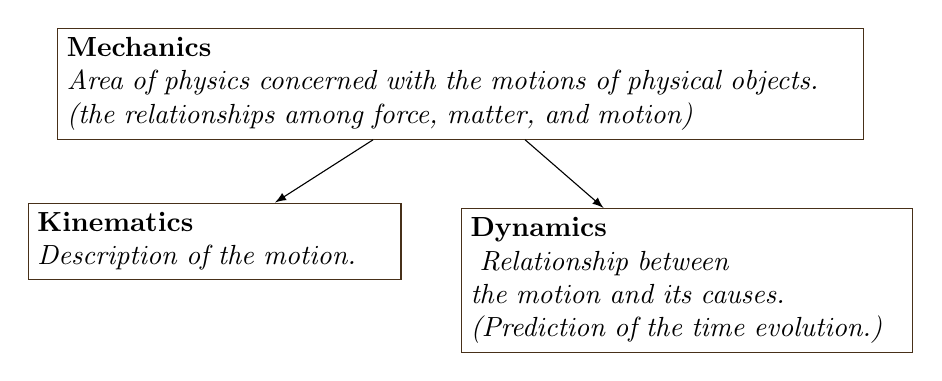
\begin{tikzpicture}
		 	\node[draw=orange!20!black!90,right,text width=10cm] (s1) at (0,0)
		    {
				{\bf Mechanics} \\
				\emph{Area of physics concerned with the motions of physical objects.\\
				(the relationships among force, matter, and motion)}		            
		     }; 
 			\node[draw=orange!20!black!90,text width=4.5cm] (t1) at (2cm,-2cm)
    		{
		   		{\bf Kinematics}
		   		\\ \emph{Description of the motion.}
	        };	
 			\node[draw=orange!20!black!90,text width=5.5cm] (t2) at (8cm,-2.5cm)
    			{
		    		{\bf Dynamics} \\
		   			\emph{ Relationship between\\ the motion and its causes.\\ (Prediction of the time evolution.)}
	        };
	        \draw[-latex] (s1) -- (t1);
        	\draw[-latex] (s1) -- (t2);
		\end{tikzpicture}
	\end{center}

	\vfill
	\begin{columns}
    	\begin{column}{.33\textwidth}
	   		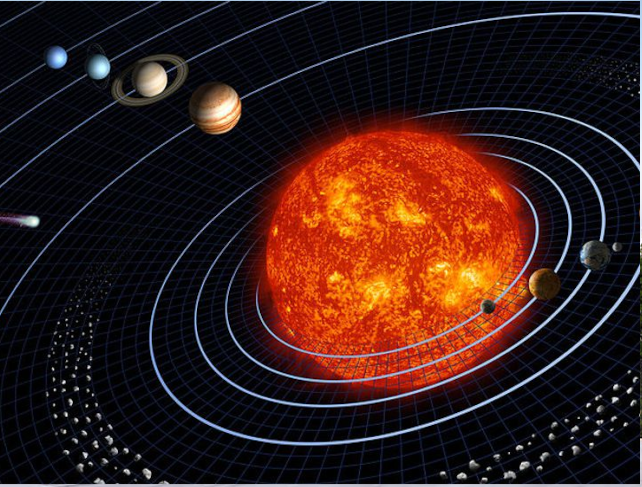
\includegraphics[width=\textwidth]{Pictures/solar} 	
		\end{column}
    	\begin{column}{.33\textwidth}
	   		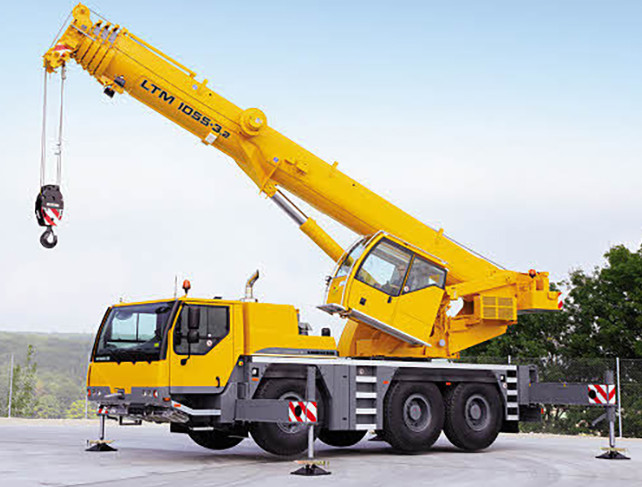
\includegraphics[width=\textwidth]{Pictures/autogru-liebherr} 	
		\end{column}
    	\begin{column}{.33\textwidth}
	   		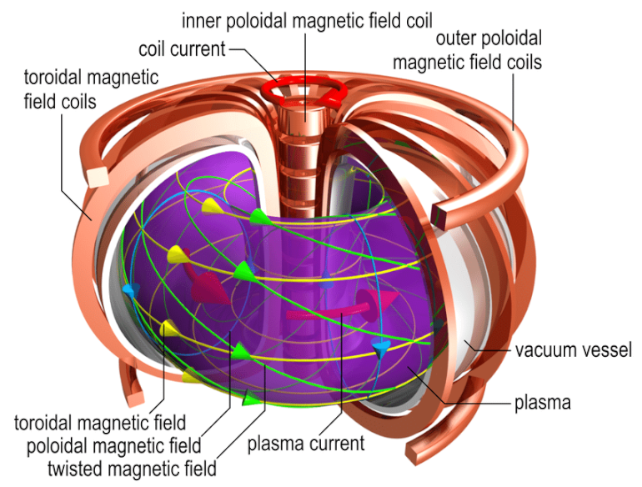
\includegraphics[width=\textwidth]{Pictures/plasma} 	
		\end{column}
	\end{columns}
\end{frame}
\note[itemize]{
	\item
}
%-------------------------------------------------------------------------------------------------------------------------------------------------

%-------------------------------------------------------------------------------------------------------------------------------------------------
\begin{frame}[t]{How does Geometry gets into Physics?}
	%
	\begin{block}{Trivial answer:}
		It appears in describing the "physical space" in which all "physical systems" are embedded.
	\end{block}
	\vfill
  	\begin{columns}<2->[T]
    	\begin{column}{.45\textwidth}
    		\begin{center}
				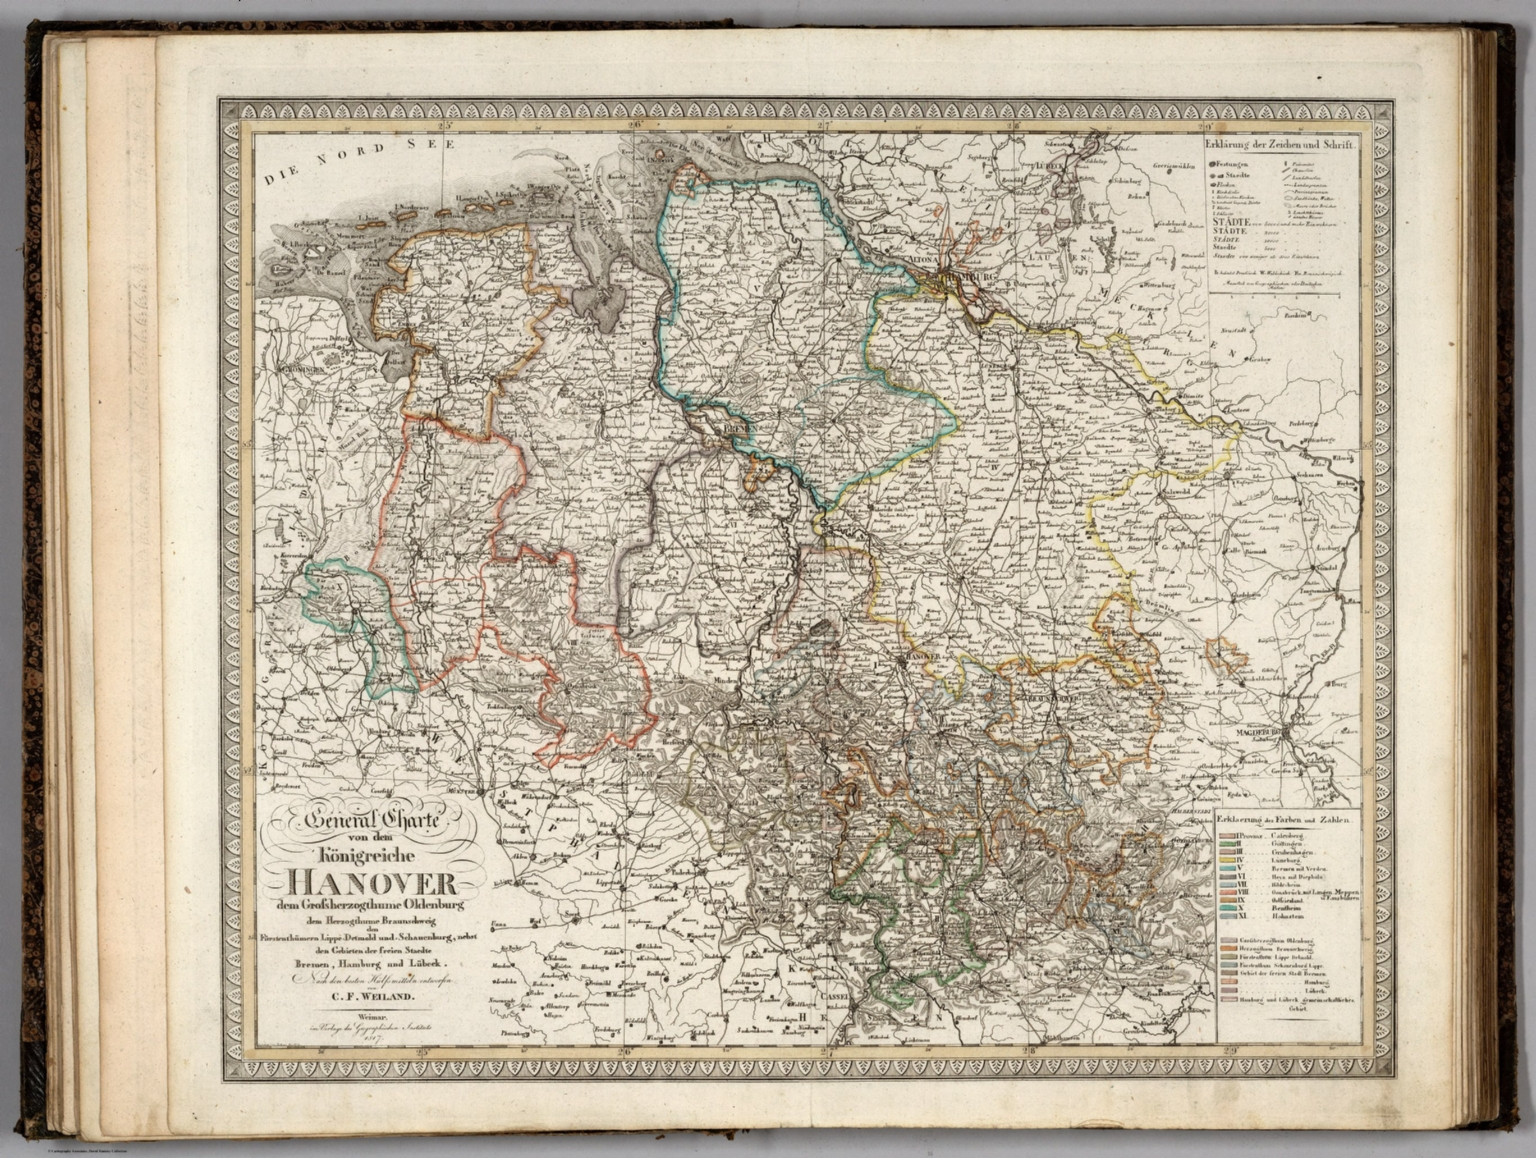
\includegraphics[width=0.9\textwidth]{Pics/map} 		
    		\end{center}
    	\end{column}
    	\begin{column}{.55\textwidth}
    		\vspace*{1em}
			\begin{block}{Historical fact:}
				Modern (intrinsic) differential geometry stemmed from a cartographic survey of the Kingdom of Hanover commissioned to Carl Friederich Gauss in 1828.		
			\end{block}
    	\end{column}
    \end{columns}
	\vfill
	\begin{alertblock}<3->{There is much more!}
		Geometry provides a powerful language to encode deep properties of physics encompassing a huge variety of mechanical systems.
	\end{alertblock}
\end{frame}
\note[itemize]{
	\item Three fundamentals concepts: Space, Body (system), Displacement.
	\item Nevertheless, the problem of measuring "Earth" is one of the oldest problem in mathematics (see \url{https://en.wikipedia.org/wiki/YBC_7289})
	\item Nel 1818 fu chiesto a Gauss di compiere la rilevazione geodetica del Regno di Hannover, associandola ai precedenti rilevamenti effettuati in Danimarca.
La cartografia dell'Hannover portò Gauss a sviluppare la geometria differenziale insieme alle potenzialità della geometria non euclidea.
}
%-------------------------------------------------------------------------------------------------------------------------------------------------

%-------------------------------------------------------------------------------------------------------------------------------------------------
\begin{frame}{What we mean by: \emph{Geometric mechanics}? (1)}
	\alert{"Geometric mechanics" is not a completely standard (widely accepted) term.} \\
	It needs some clarification...
	\vfill
	\pause
	The idea of intermarrying geometry with mechanics has a noble father...
	\begin{columns}[T]
		\begin{column}{.4\textwidth}
			\center
			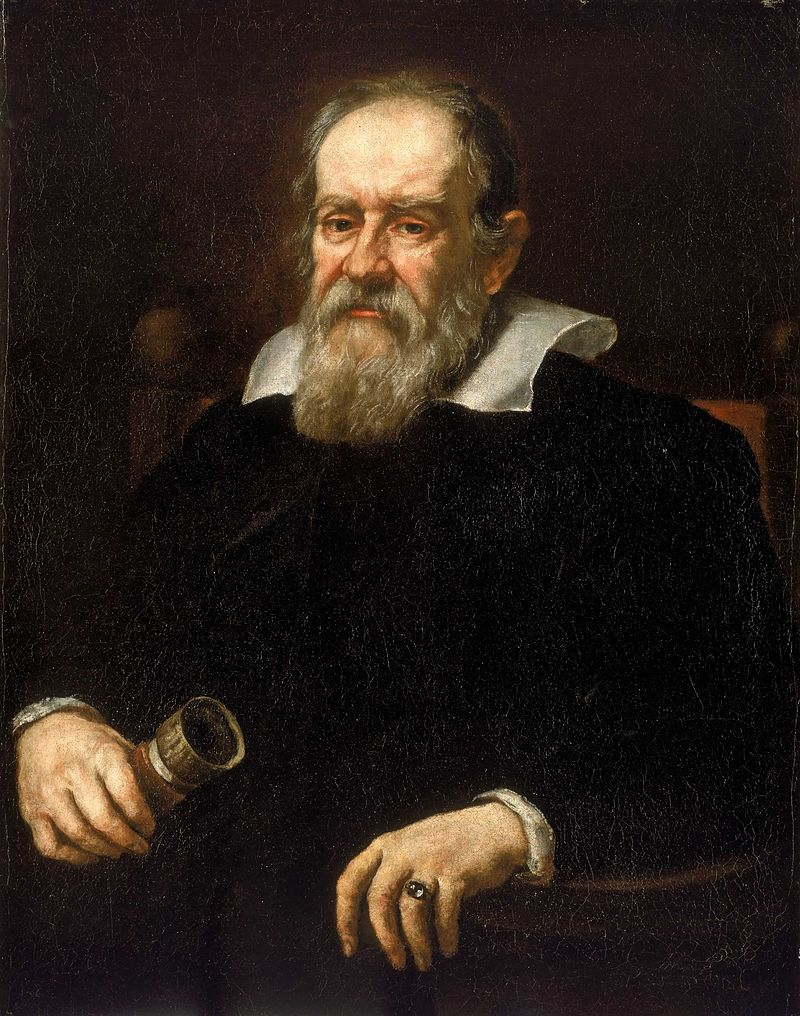
\includegraphics[width=0.8\textwidth]{Pictures/FFat/Galileo} 
		\end{column}
		\begin{column}{.6\textwidth}
			\only<2>{
			\begin{quotation}
			{\footnotesize 
				«La filosofia è scritta in questo grandissimo libro che continuamente ci sta aperto innanzi a gli occhi (io dico {\bf l'universo}), ma non si può intendere se prima non s'impara a intender la lingua, e conoscer i caratteri, ne' quali è scritto. 
				Egli {\bf è scritto in lingua matematica, e i caratteri son triangoli, cerchi, ed altre figure geometriche}, senza i quali mezzi è impossibile a intenderne umanamente parola; senza questi è un aggirarsi vanamente per un oscuro laberinto.»
			}
			\end{quotation}
			}
			\only<3->{		
			\begin{quotation}
			{\footnotesize 
				«Philosophy {\bf [nature]} is written in that great book which ever is before our eyes -- I mean the universe -- but we cannot understand it if we do not first learn the language and grasp the symbols in which it is written. 
				The book {\bf is written in mathematical language, and the symbols are triangles, circles and other geometrical figures}, without whose help it is impossible to comprehend a single word of it; without which one wanders in vain through a dark labyrinth.»		
			}
			\end{quotation}	
			}
			(Galileo Galilei, Il Saggiatore, 1623)	
		\end{column}	
	\end{columns}	
\end{frame}
\note[itemize]{
	\item Praticamente l'idea è vecchia quanto la scienza.f
}
%-------------------------------------------------------------------------------------------------------------------------------------------------


%-------------------------------------------------------------------------------------------------------------------------------------------------
\begin{frame}{What we mean by: \emph{Geometric mechanics}? (2)}
	What we mean \underline{here} is:
	\\
	the modern discipline originated in the 60s by the work of these mathematicians%gentlemen
	
	\vfill
	\begin{columns}[T]
		\begin{column}{.2\textwidth}
			\center
			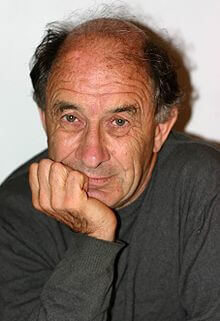
\includegraphics[width=0.8\textwidth]{Pictures/FFat/arnold}
			Vladimir \\ 
			Arnold
		\end{column}
		\begin{column}{.2\textwidth}
			\center
			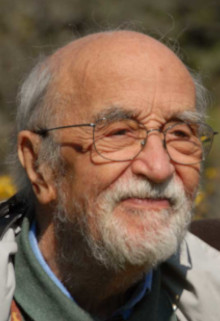
\includegraphics[width=0.8\textwidth]{Pictures/FFat/souriau} 
			Jean-Marie \\			
			Souriau
		\end{column}
		\begin{column}{.2\textwidth}
			\center
			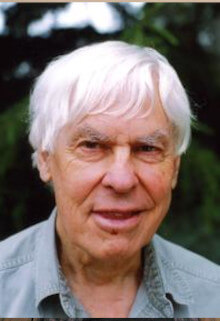
\includegraphics[width=0.8\textwidth]{Pictures/FFat/smale}
			Stephen \\
			Smale
		\end{column}
		\begin{column}{.2\textwidth}
			\center
			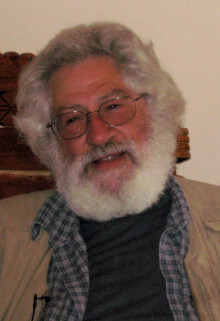
\includegraphics[width=0.8\textwidth]{Pictures/FFat/abraham} 
			Ralph \\			
			Abraham
		\end{column}
		\begin{column}{.2\textwidth}
			\center
			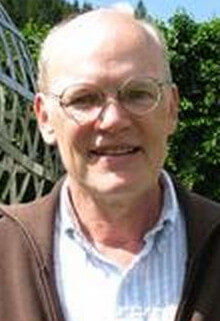
\includegraphics[width=0.8\textwidth]{Pictures/FFat/marsden} 
			Jerrold \\
			Marsden
		\end{column}		
	\end{columns}	

	\pause
	\vfill
	\begin{block}<1->{Introduced as a branch of \emph{(applied) Mathematics}}
			Employs modern (differential) geometry to the description of dynamical systems.	
	\end{block}


\end{frame}
\note[itemize]{
	\item %\href{https://en.wikipedia.org/wiki/Geometric_mechanics#History}{wiki}
		Arnold's fundamental work showed that Euler's equations for the free rigid body are the equations for geodesic flow on the rotation group SO(3) and carried this geometric insight over to the dynamics of ideal fluids, where the rotation group is replaced by the group of volume-preserving diffeomorphisms. 
	\item Smale's paper on Topology and Mechanics investigates the conserved quantities arising from Noether's theorem when a Lie group of symmetries acts on a mechanical system, and defines what is now called the momentum map (which Smale calls angular momentum), and he raises questions about the topology of the energy-momentum level surfaces and the effect on the dynamics. 
	\item Souriau also considered the conserved quantities arising from the action of a group of symmetries, but he concentrates more on the geometric structures involved (for example the equivariance properties of this momentum for a wide class of symmetries), and less on questions of dynamics.
	\item These ideas leads to the seminal book: \emph{Foundations of Mechanics} by Abraham and Marsden (1978).
	\item 		{physical è un po' restrittivo, diciamo sistemi che evolvono?}	
		{dynamical systems: non solo meccanica classica non relativistica non quantistica!}

}
%-------------------------------------------------------------------------------------------------------------------------------------------------

%-------------------------------------------------------------------------------------------------------------------------------------------------
\begin{frame}[t]{What is... \emph{Geometric Mechanics?}}
		\begin{block}{As an approach to \emph{Rational Mechanics}:}
			\begin{itemize}
				\item \textbf{Key idea:} make use of geometry to completely encode a physical system's mechanical properties regardless of the coordinate system employed.
				\item \textbf{The goal:} reconstruction of the physical observable quantities of interest from these abstract mathematical setting.
				\item \textbf{Advantage:} formalize the system's relevant structure in order to:
					\begin{itemize}
						\item[-] simplify the analytical or numerical solution of motion equations;
						\item[-] derive its quantum or relativistic counterpart.		
					\end{itemize}									
			\end{itemize}
		\end{block}
		%
		\vfill
		\pause
		\begin{block}{Some direct applications:}
			\vspace{-0.5em}
			\begin{columns}
		    	\begin{column}{.45\textwidth}
					\begin{itemize}
						\item[-] Theoretical chemistry
						\item[-] Control theory
						\item[-] Image processing
					\end{itemize}
				\end{column}
		    	\begin{column}{.45\textwidth}
					\begin{itemize}
						\item[-] Mathematical finance
						\item[-] Earth sciences
						\item[-] Robotics
					\end{itemize}
				\end{column}
			\end{columns}
		\end{block}
		\vfill
		\pause
		\begin{block}{Three cornerstones of geometric mechanics}
	\begin{center}
		%\scalebox{.8}{%
		{
		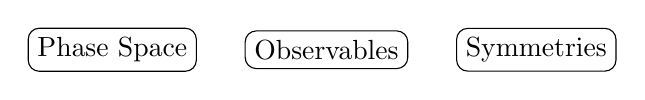
\begin{tikzpicture}[>=stealth,every node/.style={shape=rectangle,draw,rounded corners},node distance=0.05\linewidth,]
	    % create the nodes
		    \node (a1) {Phase Space};
		    \node (a2)[right =of a1] {Observables};
		    \node (a3)[right =of a2] {Symmetries};
		\end{tikzpicture}
%				\node [text width=0.6\linewidth, rectangle,draw,right of=lhs] (rhs) {Lie subgroup \\$G \subset Diff(M)$};
		}			
	\end{center}		
		\end{block}


		%https://en.wikipedia.org/wiki/Geometric_mechanics

		%http://www10.mathematik.uni-wuerzburg.de/index.php?path=research/maphy
	\end{frame}
	\note[itemize]{
		\item the geometric language permits to formalize the evolution of system composed of both quantum and classical degree of freedom (mesoscopic scale)
		\item Lessig: 
		In our discussion we only considered classical mechanical systems. However,
the theory applies to a diverse array of fields and disciplines ranging from quantum mechanics at the smallest scales to relativistic astrophysics at the largest, and applications can be found in areas such as image processing, space mission design, marine animal propulsion, mathematical finance, rising eggs, oceanography, plasma physics, falling cat phenomena, and many more. In its contemporary formulation using the rich toolbox of modern geometry, geometric mechanics provides thereby a surprisingly unified perspective on all these systems.
		\item Manifolds arise naturally in the description of classical mechanical systems.
		\item Geometrization of mechanics yields an inherent intuition to differential geometry structures (manifolds, charts, vectors ...).
		\item Encoding a classical mechanical system via a precise mathematical framework allows  to the relevant structures of our physical theories to emerge.
		\item A sound mathematical foundation provides a solid ground where to perform axiomatization of physical theories, quantization and "relativization".
		\item With a slight refinement of the mathematical language, also systems with continuous degrees of freedom (fluid and fields) can be accommodated within this geometrical framework as well.
		\item This framework could be adapted directly to ordinary quantum mechanical systems (e.g. Bloch sphere).
		\item There are also  direct applications!!! (if you are that kind of person .... :P )
				(if aiming to a complete mathematical foundation it's not enough for you...)
	}
%-------------------------------------------------------------------------------------------------------------------------------------------------




%-------------------------------------------------------------------------------------------------------------------------------------------------

%-------------------------------------------------------------------------------------------------------------------------------------------------
\subsection{Phase Space}
\subcheckpoint	
%-------------------------------------------------------------------------------------------------------------------------------------------------
	%+----------------------------------------------------------------------------+
%| SLIDES: 
%| Chapter: Configuration Space
%| Author: Antonio miti
%| Event: Phd Colloquium - What is ... Geometric mechanics?
%+----------------------------------------------------------------------------+

%- HandOut Flag -----------------------------------------------------------------------------------------
\makeatletter
\@ifundefined{ifHandout}{%
  \expandafter\newif\csname ifHandout\endcsname
}{}
\makeatother

%- D0cum3nt ----------------------------------------------------------------------------------------------
\documentclass[beamer,10pt]{standalone}   
%\documentclass[beamer,10pt,handout]{standalone}  \Handouttrue  

\ifHandout
	\setbeameroption{show notes} %print notes   
\fi

	
%- Packages ----------------------------------------------------------------------------------------------
\usepackage{custom-style}
\usetikzlibrary{positioning}
\usepackage{multicol}


%--Beamer Style-----------------------------------------------------------------------------------------------
\usetheme{toninus}
\usepackage{animate}
\usetikzlibrary{positioning, arrows}
\usetikzlibrary{shapes}

\begin{document}
%-------------------------------------------------------------------------------------------------------------------------------------------------
\begin{frame}{Phase Space via Configuration Space}
	\begin{itemize}
	\item To introduce the notion of {\bf phase space} it is useful to start from the auxiliary concept of {\bf configuration space}.
	\end{itemize}

	\vfill
	\begin{itemize}
		\item<2-> this notion is based on three \emph{primitive concepts}:
	\end{itemize}
	\onslide<2->{
		\begin{center}
			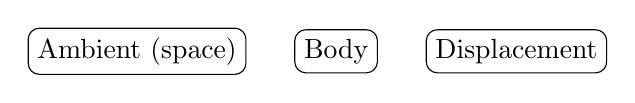
\begin{tikzpicture}[>=stealth,every node/.style={shape=rectangle,draw,rounded corners},node distance=0.05\linewidth,]
		    % create the nodes
			    \node[] (a1) {Ambient (space)}; %Physical space
			    \node[] (a2)[right =of a1] {Body}; %(Physical) system
			    \node[] (a3)[right =of a2] {Displacement}; %configuration
			\end{tikzpicture}
		\end{center}
	}
\end{frame}
\note[itemize]{
	\item In molte presentazioni di nozioni matematiche per concetto primitivo o nozione primitiva si intende un concetto che, per la propria semplicità ed intuitività, si rinuncia a definire mediante termini e concetti già definiti all'interno di un sistema formale, e che al contrario si sceglie di sfruttare per formulare la definizione di altri concetti; pertanto un concetto primitivo si accetta senza spiegazioni perché il suo significato è ovvio.
}
%-------------------------------------------------------------------------------------------------------------------------------------------------


%-------------------------------------------------------------------------------------------------------------------------------------------------
\begin{frame}[t]{Configuration Space: the Ambient}
	\begin{center}
		
\begin{tikzpicture}[>=stealth,every node/.style={shape=rectangle,draw,rounded corners},node distance=0.05\linewidth,]
	    % create the nodes
		    \node[red] (a1) {Ambient (space)}; %Physical space
		    \node[gray] (a2)[right =of a1] {Body}; %(Physical) system
		    \node[gray] (a3)[right =of a2] {Displacement}; %configuration
		\end{tikzpicture}	
	\end{center}
	\begin{columns}
		\begin{column}[T]{0.5\textwidth}
			\begin{itemize}
				\item The physical space, our universe.
				\item It is the stage on which the act of dynamics takes place.
			\end{itemize}
			\vspace{1em}
			\onslide<2->{					
				\begin{exblock}
					Consider a laboratory.
				\end{exblock}
			}
			\vspace{1em}
			\onslide<3->{
				\begin{mathblock}
					is the Euclidean space $E=\mathbb{R}^3$.
					\\				
					(fixed a \emph{Galilean observer}) 
				\end{mathblock}
			}		
		\end{column}
		\begin{column}[T]{0.5\textwidth}
			\onslide<2->{
				\begin{center}
					
\includegraphics[width=\textwidth]{Pictures/emptylab}
				\end{center}
			}
		\end{column}
	\end{columns}
\end{frame}
\note[itemize]{
	\item
}
%-------------------------------------------------------------------------------------------------------------------------------------------------


%-------------------------------------------------------------------------------------------------------------------------------------------------
\begin{frame}[t]{Configuration Space: the Body}
	\begin{center}
		
\begin{tikzpicture}[>=stealth,every node/.style={shape=rectangle,draw,rounded corners},node distance=0.05\linewidth,]
	    % create the nodes
		    \node[gray] (a1) {Ambient (space)}; %Physical space
		    \node[red] (a2)[right =of a1] {Body}; %(Physical) system
		    \node[gray] (a3)[right =of a2] {Displacement}; %configuration
		\end{tikzpicture}
	\end{center}

	\begin{columns}
		\begin{column}[T]{0.5\textwidth}
			\begin{itemize}
				\item it is a bulk of matter, a portion of the ambient, we wish to study.
			\end{itemize}
								
			\vspace{1em}
			\only<2->{			
				\begin{exblock}
					Consider the bob of a rigid pendulum.
				\end{exblock}
			}

			\vspace{1em}
			\only<3->{
				\begin{mathblock}
					\begin{columns}
						\begin{column}{0.025\textwidth}
						\end{column}
						\begin{column}[T]{0.5\textwidth}
							is a submanifold $B\hookrightarrow E$ with boundary
							\vspace{-.5em}
							\begin{center}
								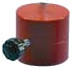
\includegraphics[width=.25\textwidth]{Pictures/bob}
							\end{center}
						\end{column}					
						\begin{column}[T]{0.45\textwidth}
							is a point in $B\in E$ (the center of mass).
							\begin{center}
								\tikz[] \node[scale=0.5,coordinate,fill=red,circle] (n1) {};	
							\end{center}						
						\end{column}							
					\end{columns}
					\begin{column}{0.025\textwidth}
					\end{column}
				\end{mathblock}
			}
			\vfill
%			\only<4->{
%				\begin{bracketbox}%{Key point:}
%					\small
%					Remind:
%					The ambient acts on the body via \emph{forces} and \emph{constraints}.
%				\end{bracketbox}
%			}	
		\end{column}
		\begin{column}[T]{0.5\textwidth}
				\begin{center}
					\includegraphics<1>[width=\textwidth]{Pictures/emptylab}
					\includegraphics<2->[width=\textwidth]{Pictures/Pendolab}					
				\end{center}
		\end{column}
	\end{columns}
\end{frame}
\note[itemize]{
	\item "è il protagonista della recita"
	\item remind the implied idea: 	The ambient acts on the body via \emph{forces} and \emph{constraints}.
}	
%-------------------------------------------------------------------------------------------------------------------------------------------------


%-------------------------------------------------------------------------------------------------------------------------------------------------
\begin{frame}[t]{Configuration Space: the displacement}
	\begin{center}
		
\begin{tikzpicture}[>=stealth,every node/.style={shape=rectangle,draw,rounded corners},node distance=0.05\linewidth,]
	    % create the nodes
		    \node[gray] (a1) {Ambient (space)}; %Physical space
		    \node[gray] (a2)[right =of a1] {Body}; %(Physical) system
		    \node[red] (a3)[right =of a2] {Displacement}; %configuration
		\end{tikzpicture}
	\end{center}

	\begin{columns}
		\begin{column}[T]{0.5\textwidth}
			\begin{itemize}
				\item is how the body is placed inside the space.
				\item configuration (spatial displacement) of the physical system admissible by the constraints.
			\end{itemize}
			\vspace{1em}
			\only<2->{
				\begin{exblock}[Pendulum]
					one of the possible positions where the bob can be placed allowed by the rod.		
				\end{exblock}
			}	
			\vspace{1em}
			\only<3->{
				\begin{mathblock}
					is a (smooth) function $B \to E$.				
				\end{mathblock}
			}					
			
		\end{column}
		\begin{column}[T]{0.5\textwidth}
			\begin{center}
				\includegraphics<1>[width=\textwidth]{Pictures/Pendolab}
				\only<2->{	
					\animategraphics[autoplay,palindrome,width=\textwidth]{5}{Pictures/pendolum-frame/pendo}{1}{9}
				}
			\end{center}
		\end{column}
	\end{columns}
\end{frame}
\note[itemize]{
	\item
}

%-------------------------------------------------------------------------------------------------------------------------------------------------

%-------------------------------------------------------------------------------------------------------------------------------------------------
\begin{frame}[t]{Configuration Space}
	%	
	\center
	\begin{zigzagbox}
		Neglect the fluff $\quad\rightsquigarrow\quad$ abstract (synthetic) mathematical setting
	\end{zigzagbox}
	
	\begin{columns}
		\begin{column}[T]{0.5\textwidth}
			\begin{itemize}
				\item<2-> Consider the set $Q$  of all the possible displacements (spatial configurations).
			\end{itemize}
			%			
			\vspace{1em}
			\onslide<3->{
				\begin{exblock}[Pendulum]
					$Q$ = 
						the locus of points on the plane with fixed distance from the pivot (the circle $S^1$).	
				\end{exblock}
			
			}			
			%			
			\vspace{1em}
			\onslide<4->{
				\alert{Upshot: $Q$ is a smooth manifold}
							
			\begin{defblock}[Configuration Space]
				Smooth manifold of all the system configurations admissible by the constraints.
			\end{defblock}			
			}
		\end{column}


		\begin{column}[T]{0.5\textwidth}
			\begin{center}
			\only<1>{				
				\resizebox{\textwidth}{!}{		
				    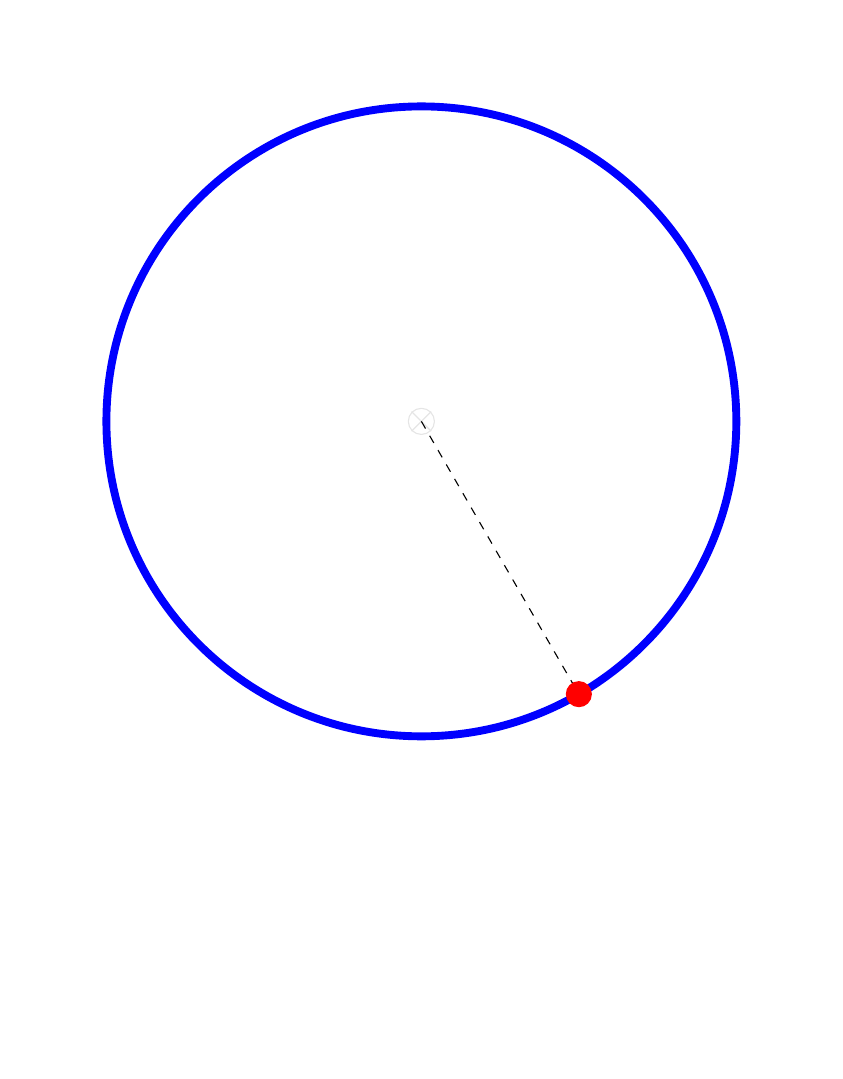
\begin{tikzpicture}
					    %frame
					    \draw[draw=none] (-5,-8) rectangle (5,5);
						% Support
						\coordinate (o) at (0,0);
						\node[cross out,draw,black!10] (0,0){};
						\node[circle,draw,black!10] (0,0){};
						% Bob's trajectory
						\draw[blue,line width=1mm,] (0,0) circle (4);
						% Rod + Bob
						\draw[dashed] (0,0) -- (-60:4) node[fill,circle,red](m){};
				    \end{tikzpicture}
				}
			}
			\only<2->{				
				\resizebox{\textwidth}{!}{		
					\pgfmathtruncatemacro\steps{50}
					\pgfmathtruncatemacro\maxtheta{30}
					\pgfmathtruncatemacro\pi{3.14}
					\begin{animateinline}[autoplay,loop]{10} % 5 fps, same as 0.2 s transduration
					  \multiframe{\steps}{i=0+1}{
					    \begin{tikzpicture}
					    \pgfmathsetmacro\fraction{\i/(\steps-1)}
						\pgfmathsetmacro\theta{\maxtheta*cos(360*\fraction)-90}
					    %frame
					    \draw[draw=none] (-5,-8) rectangle (5,5);
						% Support
						\coordinate (o) at (0,0);
						\node[cross out,draw,black!10] (0,0){};
						\node[circle,draw,black!10] (0,0){};
						% Bob's trajectory
						\draw[blue,line width=1mm] (0,0) circle (4);
						% Rod + Bob
						\draw[dashed] (0,0) -- (\theta:4) node[fill,circle,red](m){};
					    \end{tikzpicture}
					  }
					\end{animateinline}
				}
			}
			\end{center}
		\end{column}
	\end{columns}
\end{frame}
\note[itemize]{
	\item
}

%-------------------------------------------------------------------------------------------------------------------------------------------------

%-------------------------------------------------------------------------------------------------------------------------------------------------
\begin{frame}[t]{Configuration Space: a slightly more difficult example}
		\center
	\begin{bracketbox}
		Double pendulum.
	\end{bracketbox}
	

	\vfill
	\only<1-3>{
		\begin{columns}[T]
			\begin{column}{0.5\textwidth}
				\begin{center}
					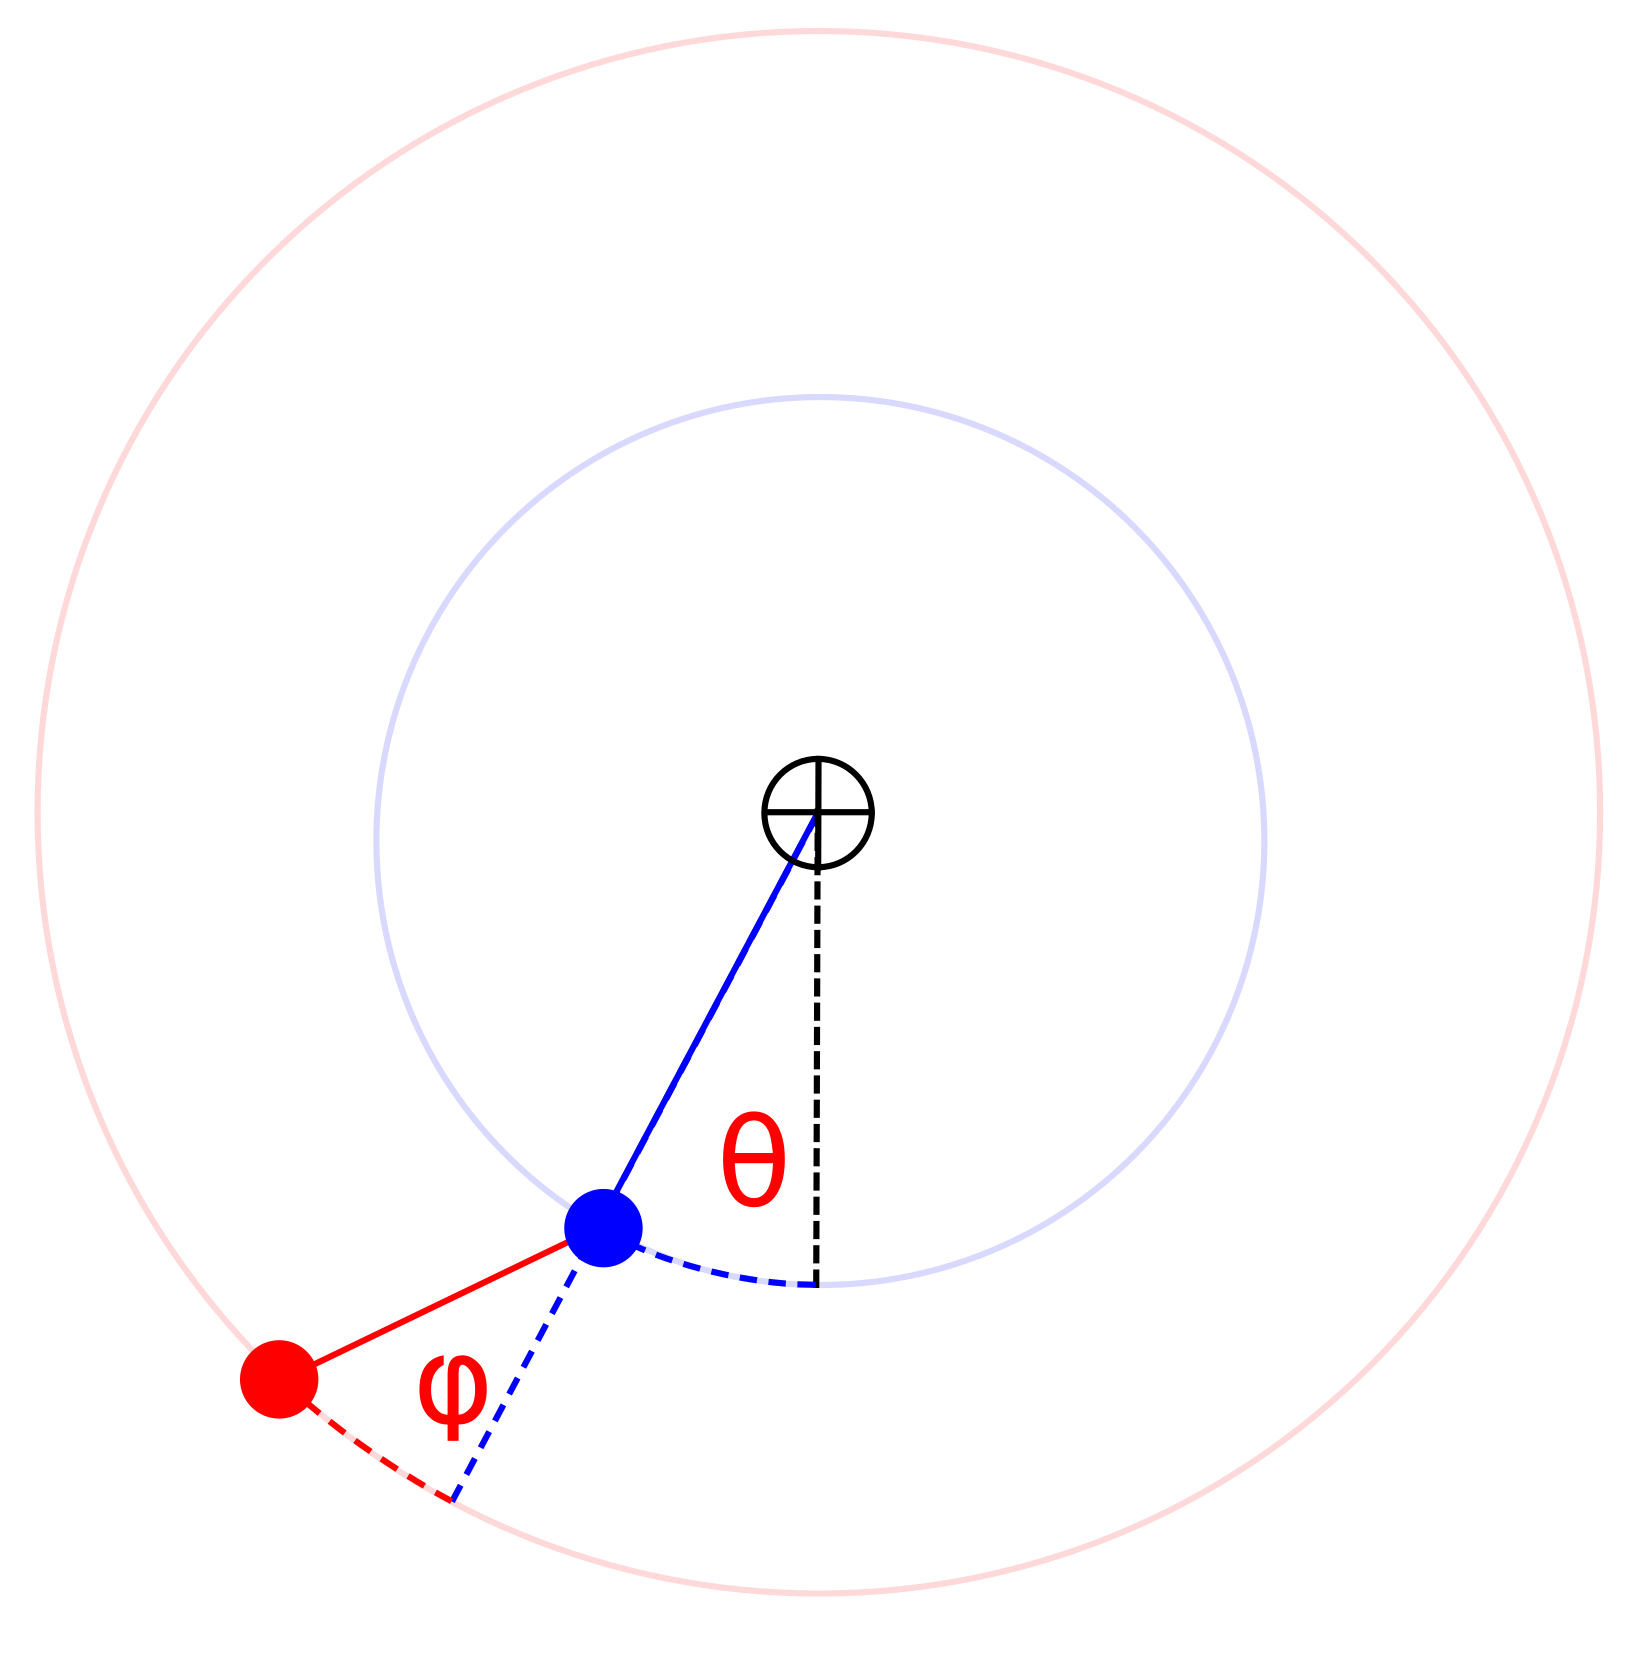
\includegraphics[width=.75\textwidth]{Pictures/bipend-abstract}	
				\end{center}
			\end{column}
			\begin{column}{0.5\textwidth}
				\begin{center}
					\only<1>{
						\noindent Toy model for:
						\begin{center}
							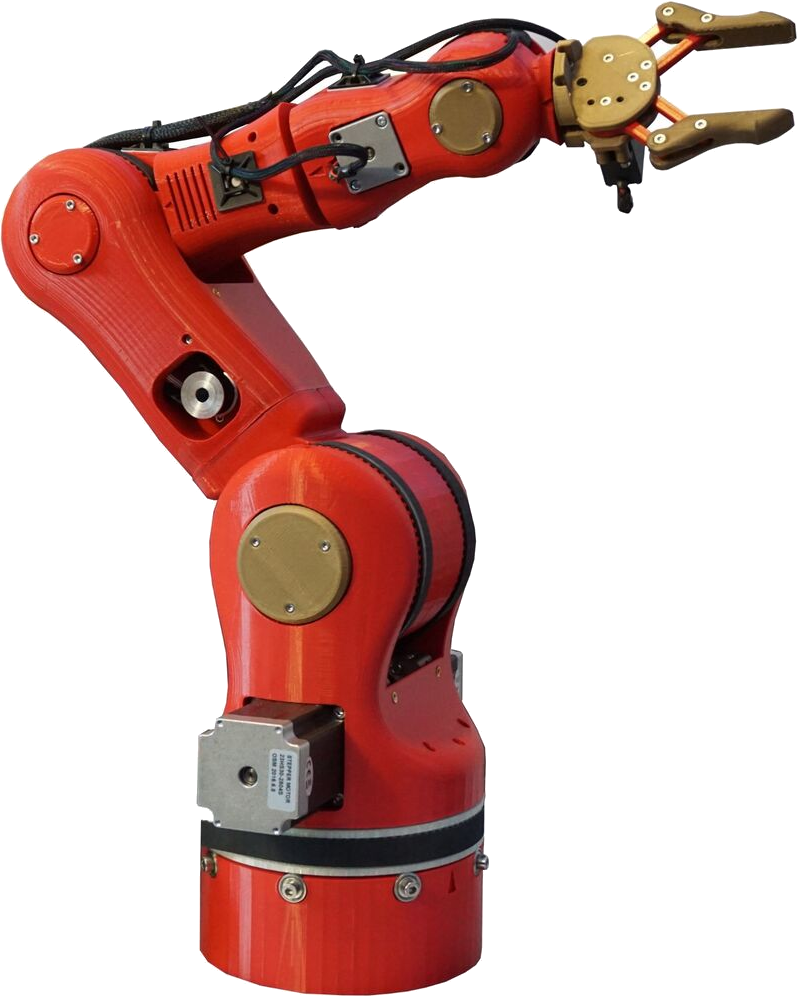
\includegraphics[width=.55\textwidth]{Pictures/robo_arm}
						\end{center}
						mechanical arms.
					}
					\only<2>{
						\noindent Toy model for:
						\begin{center}
							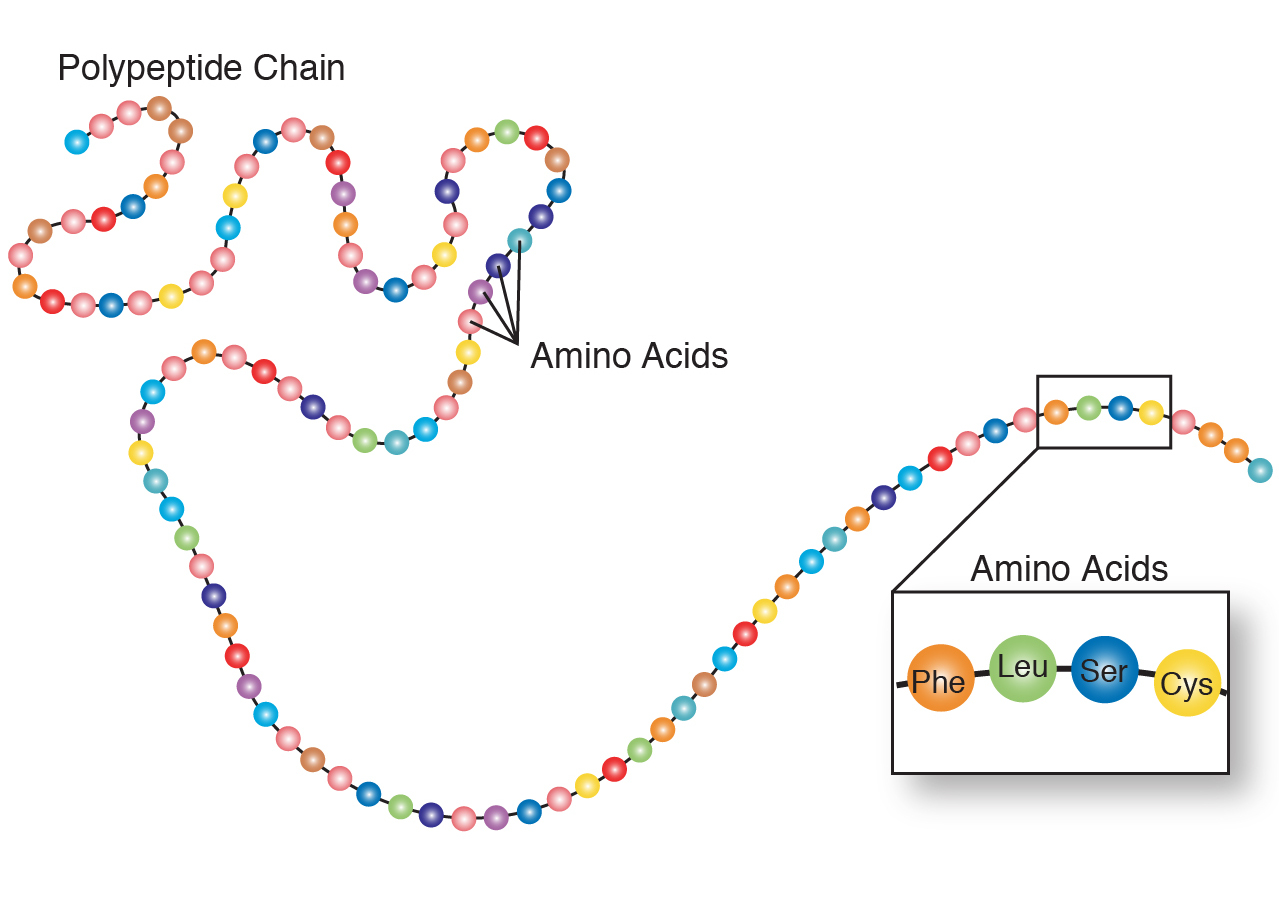
\includegraphics[width=.65\textwidth]{Pictures/amino_acids}
						\end{center}
						Proteins (amino acid chains).	
					
					}
					\only<3>{
						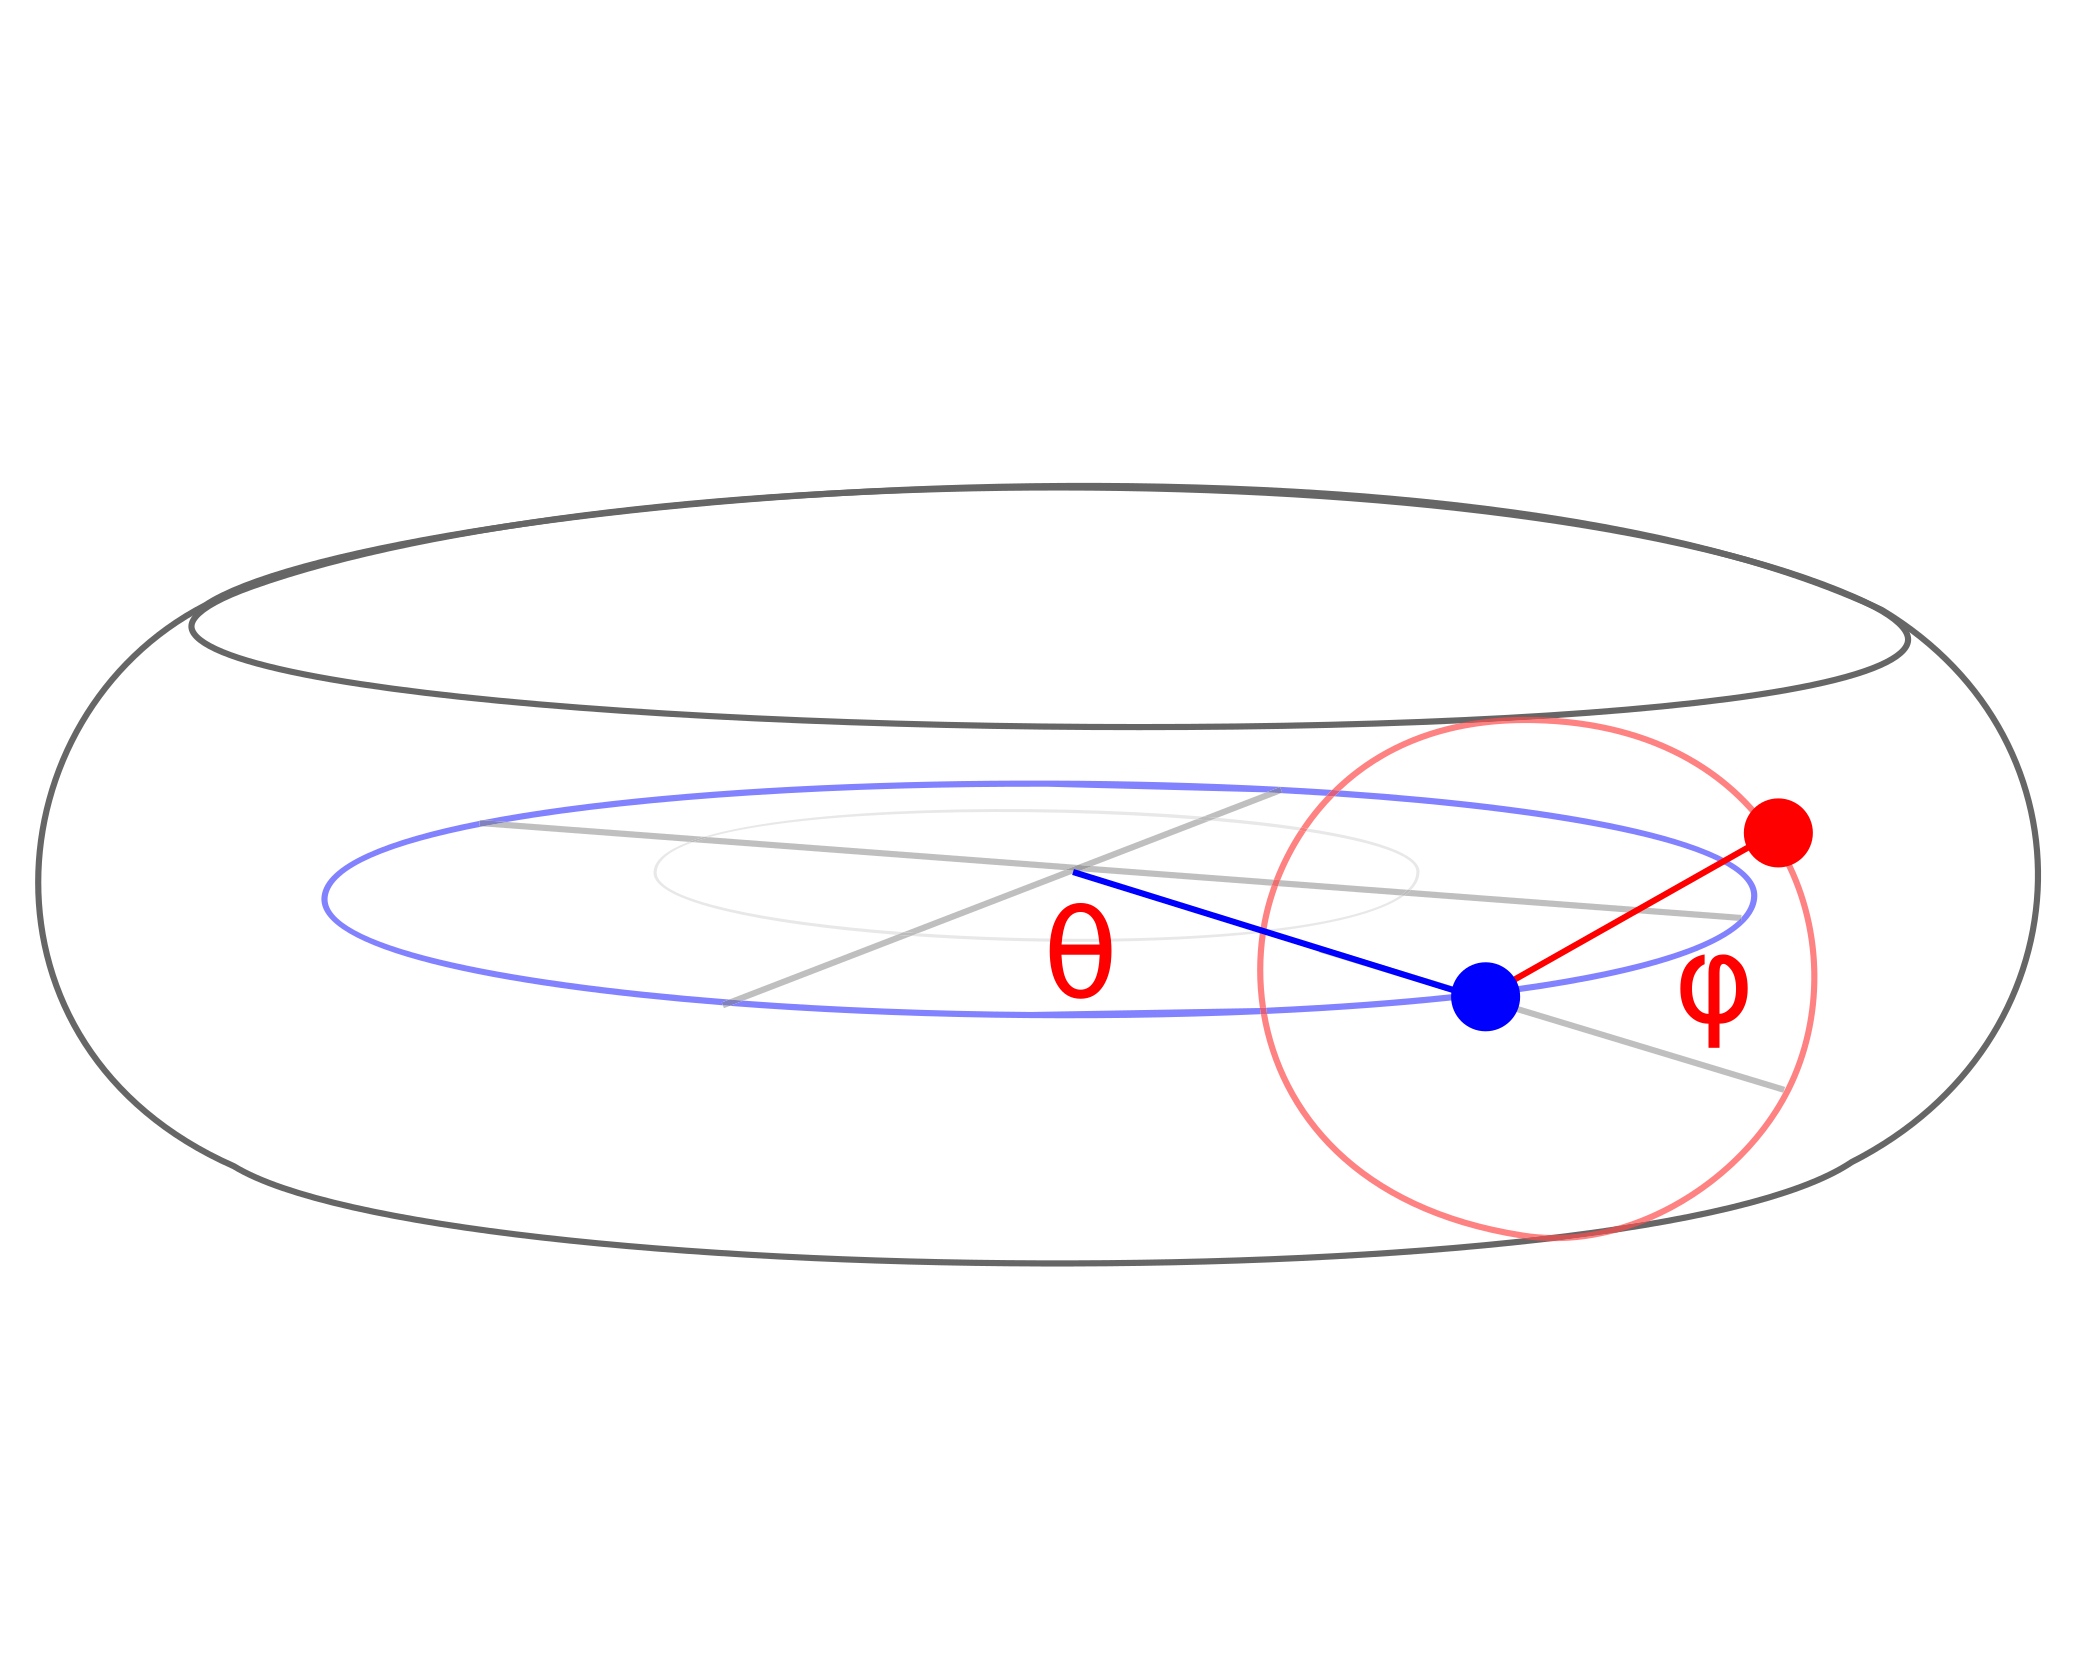
\includegraphics[width=.75\textwidth]{Pictures/bipend-phase}	
					}
				\end{center}
			\end{column}
		\end{columns}	
	}
	\only<4->{
		\animategraphics[autoplay,palindrome,width=\textwidth]{5}{Pictures/lessig-pibend-frame/bipend-}{2}{6}
	}
	\vfill
	\onslide<3->{\center\alert{Configuration space is a Torus}}


\end{frame}
\note[itemize]{
	\item per quanto sia un toy model è il primo passo per modellizzare una proteina. (Catena di amminoacidi posti a distanza pressochè costante fra di loro)
	\item This case (bi-pendulum) examplify how constraints can be enforced intrinsically choosing an appropriate geometric framework. (2-coordinates instead of the 4 x-y coordinates needed to fix the two endopoints.

}
%-------------------------------------------------------------------------------------------------------------------------------------------------

\end{document}
	%- HandOut Flag -----------------------------------------------------------------------------------------
\newif\ifHandout

%- D0cum3nt ----------------------------------------------------------------------------------------------
\documentclass[beamer,10pt]{standalone}   
%\documentclass[beamer,10pt,handout]{standalone}  \Handouttrue  

%- HandOut Flag -----------------------------------------------------------------------------------------
\ifHandout
	\setbeameroption{show notes} %print notes   
\fi

	
%- Packages ----------------------------------------------------------------------------------------------
\usepackage{custom-style}
\usetikzlibrary{positioning}
\usepackage{multicol}


%--Beamer Style-----------------------------------------------------------------------------------------------
\usetheme{toninus}
\usepackage{animate}
\usetikzlibrary{positioning, arrows}
\usetikzlibrary{shapes}
\usepackage{ifthen}

\begin{document}
%-------------------------------------------------------------------------------------------------------------------------------------------------
\begin{frame}{Phase Space}
\begin{columns}[T]
	\begin{column}{0.5\textwidth}
		\begin{center}
			\resizebox{\textwidth}{!}{		
				\pgfmathtruncatemacro\steps{50}
				\pgfmathtruncatemacro\maxtheta{30}
				\pgfmathtruncatemacro\pi{3.14}
				\begin{animateinline}[autoplay,loop]{10} % 5 fps, same as 0.2 s transduration
				  \multiframe{\steps}{i=0+1}{
				    \begin{tikzpicture}
				    \pgfmathsetmacro\fraction{\i/(\steps-1)}
					\pgfmathsetmacro\theta{\maxtheta*cos(360*\fraction)-90}
					\pgfmathsetmacro\v{-1*sin(360*\fraction)}
				
				    %frame
				    \draw[draw=none] (-6,-8) rectangle (6,6);		
					% Support
					\coordinate (o) at (0,0);
					\node[cross out,draw,black!10] (0,0){};
					\node[circle,draw,black!10] (0,0){};
					% Bob's trajectory
					\draw[blue,line width=1mm] (0,0) circle (4);
					% Rod + Bob
					\draw[dashed] (0,0) -- (\theta:4) node[fill,circle,red](m){};

					% Velocity
					\ifthenelse{\equal{\i}{0}}
           			{}
           			{\draw[-latex,green!80!black,line width=1mm] (m) -- node[green!80!black,below right]{$\vec{v}$}($(m)!\v!-90:(o)$);}
				    \end{tikzpicture}
				  }
				\end{animateinline}
			}
		\end{center}
	\end{column}
	\begin{column}{0.5\textwidth}
		\begin{itemize}
			\item Knowing the position is not sufficient to determine the evolution of the system.
			\item (Displacement encode statics, one must know how configurations evolves in time)
			\item One needs to know also the velocity (or better, the momentum).
		\end{itemize}

		\vspace{1em}
		\onslide<2->{
			\begin{upshotblocksimp}
				Upshot:
				Configurations $\neq$ \emph{States}
			\end{upshotblocksimp}			
		}
	\end{column}
\end{columns}
\end{frame}
\note[itemize]{
	\item
}
%-------------------------------------------------------------------------------------------------------------------------------------------------

%-------------------------------------------------------------------------------------------------------------------------------------------------
\begin{frame}{Phase Space}
\begin{columns}[T]
	\begin{column}{0.5\textwidth}
		\begin{center}
			\resizebox{\textwidth}{!}{
				\begin{tikzpicture}
					\node[draw=none] (o) at (0, 0) {o};
				    %frame
				    \draw[draw=none] (-6,-8) rectangle (6,6);				
					\draw[draw=none](0,0)--(-90:4)node[circle, fill, minimum size=5pt,
				              inner sep=0pt, outer sep=0pt](p){};
					\draw[green,line width=1mm] ($ (p)!3.5cm!90:(o) $) -- ($ (p)!3.5cm!270:(o) $);
					\draw[green,dashed,line width=1mm] ($ (p)!4.5cm!90:(o) $) -- ($ (p)!4.5cm!270:(o) $);
					\draw[blue,line width=1mm] (0,0) circle (4);
				\end{tikzpicture}
			}
			%
		\end{center}
	\end{column}
	\begin{column}{0.5\textwidth}
 		\begin{itemize}
 			\item consider {\bf a} configuration.
 			\item all possible velocities are encoded by points on the tangent line at the given configuration \\(\emph{Tangent space}).
 		\end{itemize}
	\end{column}
\end{columns}
\end{frame}
\note[itemize]{
	\item
}
%-------------------------------------------------------------------------------------------------------------------------------------------------

%-------------------------------------------------------------------------------------------------------------------------------------------------
\begin{frame}{Phase Space}
\begin{columns}[T]
	\begin{column}{0.5\textwidth}
		\begin{center}
			\only<1>{
			\resizebox{\textwidth}{!}{
				\begin{tikzpicture}
					\node[draw=none] (o) at (0, 0) {o};
				    %frame
				    \draw[draw=none] (-6,-8) rectangle (6,6);						
					\foreach \x in {0,30,...,360}{
						\draw[draw=none](0,0)--(\x:4)node[circle, fill, minimum size=5pt,
					              inner sep=0pt, outer sep=0pt](p){};
					\draw[green,line width=1mm] ($ (p)!3.5cm!90:(o) $) -- ($ (p)!3.5cm!270:(o) $);
					\draw[green,dashed,line width=1mm] ($ (p)!4.5cm!90:(o) $) -- ($ (p)!4.5cm!270:(o) $);
					}
						\draw[blue,line width=1mm] (0,0) circle (4);
				\end{tikzpicture}
			}}
			%
			\only<2->{
			\resizebox{.7\textwidth}{!}{
				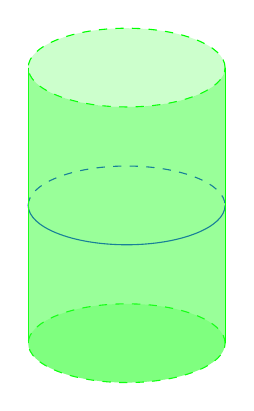
\begin{tikzpicture}
					\draw[green,dashed,fill=green!20] (0,0) ellipse (1.25 and 0.5);
					\draw [blue](-1.25,-1.75) arc (180:360:1.25 and 0.5);
					%\draw [blue,dashed] (-1.25,-3.5) arc (180:360:1.25 and -0.5);
					\draw[green,dashed,fill=green!20] (0,-3.5) ellipse (1.25 and 0.5);
					\draw [blue,dashed] (-1.25,-1.75) arc (180:360:1.25 and -0.5);
					\draw [green](-1.25,0) -- (-1.25,-3.5);
					\draw [green](1.25,-3.5) -- (1.25,0);  
					\fill [green!80,opacity=0.5] (-1.25,0) -- (-1.25,-3.5) arc (180:360:1.25 and 0.5) -- (1.25,0) arc (0:180:1.25 and -0.5);
				\end{tikzpicture}		
%				\begin{tikzpicture}
%				  \node[cylinder,draw=black,thick,aspect=0.7,minimum height=4cm,minimum width=2.5cm,shape border rotate=90,cylinder uses custom fill, cylinder body fill=green!30,cylinder end fill=green!10] (A) {\phantom{A}};
%				  \draw[dashed]
%				    let \p1 = ($ (A.after bottom) - (A.before bottom) $),
%				        \n1 = {0.5*veclen(\x1,\y1)-\pgflinewidth},
%				        \p2 = ($ (A.bottom) - (A.after bottom)!.5!(A.before bottom) $),
%				        \n2 = {veclen(\x2,\y2)-\pgflinewidth}
%				  in
%				    ([xshift=-\pgflinewidth] A.before bottom) arc [start angle=0, end angle=180,
%				    x radius=\n1, y radius=\n2];
%				\end{tikzpicture}	
}
			}
		\end{center}
	\end{column}
	\begin{column}{0.5\textwidth}
		\vspace{1.5em}
 		\begin{itemize}
 			\item Consider {\bf all possible} configurations.
 			\item Collect all possible pairs of position/momentum.
 			%\item points on the \emph{Tangent space}
 		\end{itemize}
		\vspace{1.5em} 		
 		\begin{itemize}
 			\item<2-> joining together all "tangent" space in a smooth and non-overlapping manner...
 		\end{itemize}
		\only<3->{
			\begin{upshotblocksimp}
				Upshot:
				We get another manifold (\emph{vector bundle}).
			\end{upshotblocksimp}					
		} 		
	\end{column}
\end{columns}
\end{frame}
\note[itemize]{
	\item  		
 		Collect all possible pair of position and momentum
 		
 		Informally, the tangent bundle of a manifold (which in this case is a circle) is obtained by considering all the tangent spaces (top), and joining them together in a smooth and non-overlapping manner (bottom).

}
%-------------------------------------------------------------------------------------------------------------------------------------------------

%-------------------------------------------------------------------------------------------------------------------------------------------------
\begin{frame}{Phase Space}
\begin{columns}[T]
	\begin{column}{0.5\textwidth}
		\begin{center}
			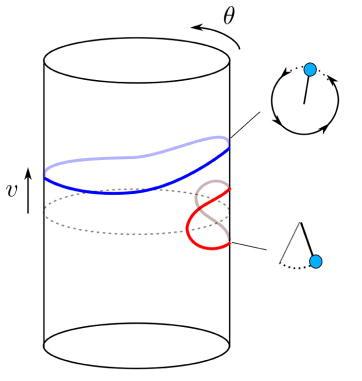
\includegraphics[width=\textwidth]{Pictures/pendo-phasespace}
		\end{center}
	\end{column}
	\begin{column}{0.5\textwidth}
 		\begin{itemize}
 			\item Consider {\bf all possible} configurations.
 			\item Collect all possible pairs of position/momentum.
 		\end{itemize}
		
		\vspace{1em}		
		\begin{defblock}[Phase Space]
			\begin{itemize}
				\item[=] collection of all \emph{states}
				\item[=] set of every possible "initial datas" (sufficient to reconstruct the motion).
			\end{itemize}
		\end{defblock}

		\vspace{1em}				
		\begin{mathblock}
			The Phase space is a \underline{symplectic} smooth manifold $(M)$.
		\end{mathblock}		
		
	\end{column}
\end{columns}
\end{frame}
\note[itemize]{
	\item You get an infinite cylinder (in the case of bipendulum I cannot picture it because we go directly into more than 2 dimensions.
	\item ho disegnato due traiettori sul fase space per mostrare come due natural motions si possono rappresentare bene qui sopra.
	\item per capire il significato di dell'aggettivo simplettico dobbiamo introdurre qualche altro interprete.

}
%-------------------------------------------------------------------------------------------------------------------------------------------------


\end{document}


%-------------------------------------------------------------------------------------------------------------------------------------------------
\subsection{Observables and time evolution}
\subcheckpoint	
%-------------------------------------------------------------------------------------------------------------------------------------------------
	%- HandOut Flag -----------------------------------------------------------------------------------------
\makeatletter
\@ifundefined{ifHandout}{%
  \expandafter\newif\csname ifHandout\endcsname
}{}
\makeatother

%- D0cum3nt ----------------------------------------------------------------------------------------------
\documentclass[beamer,10pt]{standalone}   
%\documentclass[beamer,10pt,handout]{standalone}  \Handouttrue  

\ifHandout
	\setbeameroption{show notes} %print notes   
\fi

	
%- Packages ----------------------------------------------------------------------------------------------
\usepackage{custom-style}
\usetikzlibrary{positioning}
\usepackage{multicol}


%--Beamer Style-----------------------------------------------------------------------------------------------
\usetheme{toninus}
\usepackage{animate}
\usetikzlibrary{positioning, arrows}
\usetikzlibrary{shapes,shapes.callouts}

\begin{document}

%-------------------------------------------------------------------------------------------------------------------------------------------------
\begin{frame}{Observables}
	An observables is:
	\vfill
	\begin{columns}[T]
		\begin{column}{0.5\textwidth}
			\begin{itemize}
				\item a procedure to read a certain quantity (a number) out of any state of the system
				\item<2-> a quantity that can be measured with a device. 
			\end{itemize}				
			%
			\vspace{.5em}
			\onslide<3->{
				\begin{exblock}[Pendulum inclination]
					Measure the inclination of the rod with a goniometer.
				\end{exblock}			
			}
			%
			\vspace{.5em}
			\onslide<4->{
				\begin{mathblock}
					Observables are given by smooth functions on the phase space $M$:
					\begin{displaymath}
						\mathcal{O}=C^{\infty}(M)~.
					\end{displaymath}
				\end{mathblock}
			}
		\end{column}
		\begin{column}{0.5\textwidth}
			\begin{center}
				\includegraphics<1>[width=.9\textwidth]{Pictures/pendo60-nogonio}
				\includegraphics<2>[width=.9\textwidth]{Pictures/pendo60}
				\includegraphics<3>[width=.9\textwidth]{Pictures/observo}
				\only<3>{
					\tikz[overlay,remember picture]
					{
						\node[ellipse callout,fill=white!50,
			               draw=black,
			               anchor=base]            
			            	 (base) at ($(current page.east)+(-5,3)$) [rotate=-0,text width=1.5cm,align=center,callout relative pointer={(-.3,-.8)}] 
			            	 {Measure: \\$\theta=\pi/3$\\$\phantom{\theta}\cong 1.05$};
					}	
				}
				\only<4>{
					\resizebox{.9\textwidth}{!}{				
						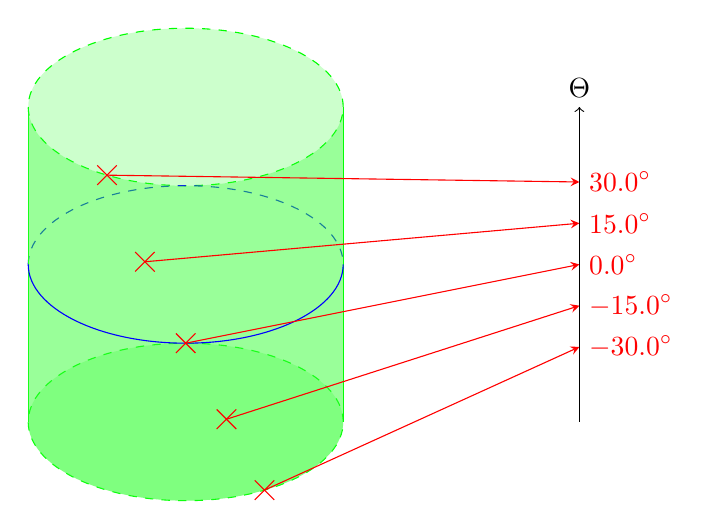
\begin{tikzpicture}
							\pgfmathtruncatemacro\steps{4}
							\pgfmathtruncatemacro\mintheta{-120}
							\pgfmathtruncatemacro\maxtheta{-60}
							\pgfmathsetmacro\deltatheta{(\maxtheta-\mintheta)/(\steps)}
							\pgfmathsetmacro\viewpitch{30}
							\pgfmathsetmacro\diam{2}
							\pgfmathsetmacro\H{4}
							\pgfmathsetmacro\deltaH{(\H)/(\steps)}
							\pgfmathsetmacro\X{\diam}
							\pgfmathsetmacro\Y{\diam*sin(\viewpitch)}	
							\pgfmathsetmacro\vel{\diam/4}	
		
							\draw[green,dashed,fill=green!20] (0,0) ellipse ({\X} and {\Y});
							%\draw [blue,dashed] (-1.25,-3.5) arc (180:360:1.25 and -0.5);
							\draw[green,dashed,fill=green!20] (0,-{\H}) ellipse ({\X} and {\Y});
							\draw [blue,dashed] (-{\X},-{.5*\H}) arc (180:360:{\X} and -{\Y});
							\draw [green](-{\X},0) -- (-{\X},-{\H});
							\draw [green]({\X},-{\H}) -- ({\X},0);  
							\fill [green!80,opacity=0.5] (-{\X},0) -- (-{\X},-{\H}) arc (180:360:{\X} and {\Y}) -- ({\X},0) arc (0:180:{\X} and -{\Y});
							\draw [blue](-\X,-{.5*\H}) arc (180:360:{\X} and {\Y});

							\foreach \i in {0,1,...,\steps}{
								\pgfmathsetmacro\h{-\i*\deltaH}
								\pgfmathsetmacro\theta{\mintheta + \i*\deltatheta}	
								\pgfmathsetmacro\thetalabel{-\theta -90}	
									
								\draw[red,-stealth] (0,\h)++({cos(\theta)*\X},{sin(\theta)*\Y}) node[draw,cross out]{}  -- (5,{pi*2*(\thetalabel)/180-\H/2})node[right] {${\thetalabel}^\circ$};
							}
							\draw[->] (5,-{\H})--(5,0) node[above] {${\Theta}$}; % ordinate
						\end{tikzpicture}	
					}
				}
			\end{center}
		\end{column}
	\end{columns}
\end{frame}
\note[itemize]{
	\item Observation /Measure, procedure to extract a number from a physical system.	E.g. a measure with a device	

}
%-------------------------------------------------------------------------------------------------------------------------------------------------

%-------------------------------------------------------------------------------------------------------------------------------------------------
\begin{frame}[t]{Hamiltonian: Energy observable}
	A certain observable takes a central role:
	\vfill
	\begin{columns}[T]
		\begin{column}{0.5\textwidth}
			\begin{defblock}[Hamiltonian observable]
				Observable measuring the total energy of the system.
				\begin{displaymath}
					H = \text{Kinetic} + \text{Potential}
				\end{displaymath}
			\end{defblock}		
			\vspace{1em}
			\onslide<2->{
				\begin{exblock}[Pendulum]
					In practical terms: $H$ is a device measuring the battery charge dissipated by a motor to lift the bob to a certain height.	
				\end{exblock}
			}			
			%
		\end{column}
		\begin{column}{0.5\textwidth}
			\begin{center}
				\onslide<2->{	
					\animategraphics[autoplay,palindrome,width=\textwidth]{1}{Pictures/pendolabenergy-}{0}{1}
				}			
			\end{center}
		\end{column}
	\end{columns}
	\vfill
	\onslide<3->{
		\begin{upshotblocksimp}
			Upshot: $H$	embodies how the ambient acts on the system and the system's inertia to respond to the external forces.
		\end{upshotblocksimp}		
	}


\end{frame}
\note[itemize]{
	\item among all possible observables "Energy" has a pivotal role:
	\item Without being too philosophica. Consider our pendulum system.
	\item \emph{potential energy} account the interaction of the "ambient" with the "body".
	\item \emph{kinetic energy} is the energy of the motion.
}
%-------------------------------------------------------------------------------------------------------------------------------------------------

%-------------------------------------------------------------------------------------------------------------------------------------------------
\begin{frame}{Symplectic structure}
	\center
	\alert{Phase spaces has a canonical \underline{symplectic structure}}
	\vfill
	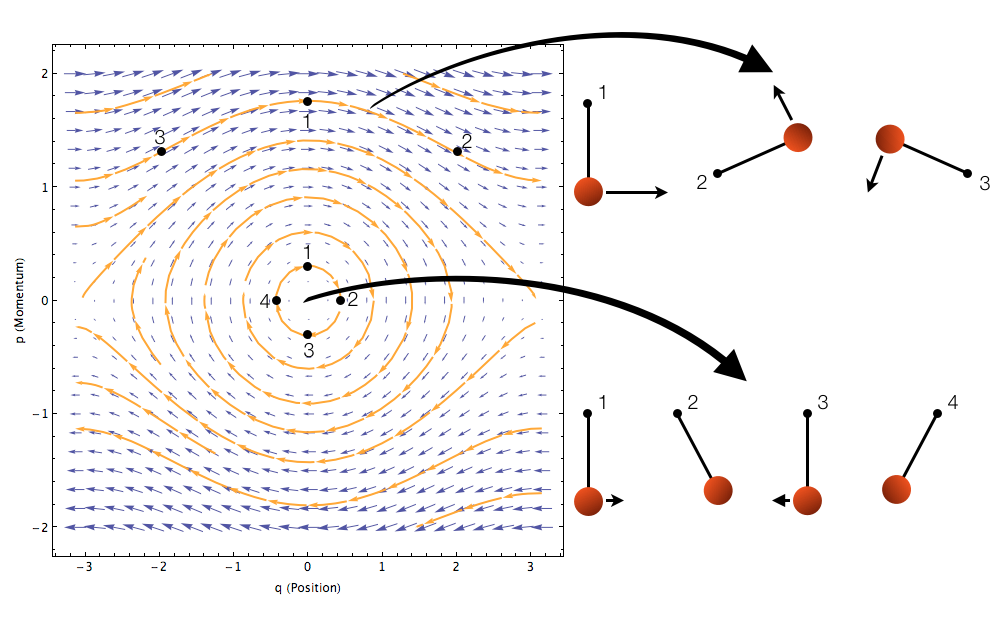
\includegraphics[width=.85\textwidth]{Pictures/pendo-hamiltonianfield}	
	\vfill
	\begin{itemize}
		\item Is  a prescription of an \emph{Hamiltonian field} $v_f$ to any observable $f$.
		\item The flow gives the evolution of the system when taking $f$ as the Hamiltonian.
		\item The Hamiltonian generates the \emph{time evolution}.
	\end{itemize}


\end{frame}
\note[itemize]{
	\item canonical i.e independent from arbitrary choices.
	\item the symplectic structure prescribes a tangent vector field to any observable quantity
}
%-------------------------------------------------------------------------------------------------------------------------------------------------

\end{document}

%-------------------------------------------------------------------------------------------------------------------------------------------------
\subsection{Symmetries}
\subcheckpoint	
%-------------------------------------------------------------------------------------------------------------------------------------------------
	%- HandOut Flag -----------------------------------------------------------------------------------------
\makeatletter
\@ifundefined{ifHandout}{%
  \expandafter\newif\csname ifHandout\endcsname
}{}
\makeatother

%- D0cum3nt ----------------------------------------------------------------------------------------------
\documentclass[beamer,10pt]{standalone}   
%\documentclass[beamer,10pt,handout]{standalone}  \Handouttrue  

\ifHandout
	\setbeameroption{show notes} %print notes   
\fi

	
%- Packages ----------------------------------------------------------------------------------------------
\usepackage{custom-style}
\usetikzlibrary{positioning}
\usepackage{multicol}


%--Beamer Style-----------------------------------------------------------------------------------------------
\usetheme{toninus}
\usepackage{animate}
\usetikzlibrary{positioning, arrows}
\usetikzlibrary{shapes}
\usetikzlibrary{calc}
\usetikzlibrary{backgrounds}
  \tikzset{
    invisible/.style={opacity=0},
    visible on/.style={alt=#1{}{invisible}},
    alt/.code args={<#1>#2#3}{%
      \alt<#1>{\pgfkeysalso{#2}}{\pgfkeysalso{#3}} % \pgfkeysalso doesn't change the path
    },
  }
 \usetikzlibrary{shapes.misc} 

  
  
\begin{document}

%-------------------------------------------------------------------------------------------------------------------------------------------------
\begin{frame}[t]{Symmetries: intuition}
	\begin{itemize}
		\item (elementary) symmetry: property of a geometric figure (shape) to be invariant under certain transformations.
	\end{itemize}
	\vfill
	\begin{center}
		\resizebox{\textwidth}{!}{			
			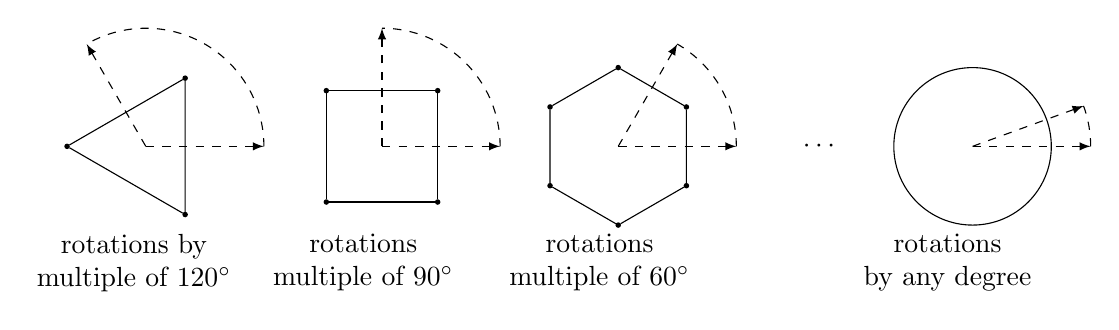
\begin{tikzpicture}
				\pgfmathtruncatemacro\R{1};
				\pgfmathsetmacro\Rext{1.5};
				\pgfmathsetmacro\dist{2*\Rext};
			    \draw[draw=none] (-\Rext,-1) rectangle (\Rext,\Rext);
		
				% Triangle
				\coordinate (o1) at (0,0);
				\draw[draw=none] (o1) -- (60:\R) node[circle, fill, minimum size=2pt,inner sep=0pt, outer sep=0pt](t1){};
				\draw[draw=none] (o1) -- (180:\R) node[circle, fill, minimum size=2pt,inner sep=0pt, outer sep=0pt](t2){};
				\draw[draw=none] (o1) -- (-60:\R) node[circle, fill, minimum size=2pt,inner sep=0pt, outer sep=0pt](t3){};
					
				\draw[dashed,-latex] (o1) -- (0:\Rext);
				\draw[dashed,-latex] (o1) -- (120:\Rext);
				\draw[dashed] (0:\Rext) arc(0:120:\Rext);
								
				\draw (t1) -- (t2) -- (t3) -- (t1);
				
				\node[below right,align=center,thick,outer sep=0pt,visible on=<2->] at (-\Rext,-1)
       				{rotations by\\ multiple of $120^\circ$};


				% Square	
				\coordinate (o2) at (\dist,0);
				\draw[draw=none] (o2) -- ++ (45:\R) node[circle, fill, minimum size=2pt,inner sep=0pt, outer sep=0pt](s1){};
				\draw[draw=none] (o2) -- ++ (135:\R) node[circle, fill, minimum size=2pt,inner sep=0pt, outer sep=0pt](s2){};
				\draw[draw=none] (o2) -- ++ (225:\R) node[circle, fill, minimum size=2pt,inner sep=0pt, outer sep=0pt](s3){};
				\draw[draw=none] (o2) -- ++ (315:\R) node[circle, fill, minimum size=2pt,inner sep=0pt, outer sep=0pt](s4){};
		
					
				\draw[dashed,-latex] (o2) -- ++ (0:\Rext);
				\draw[dashed,-latex] (o2) -- ++ (90:\Rext);
				\draw[dashed] (o2)++(0:\Rext) arc (0:90:\Rext);
								
				\draw (s1) -- (s2) -- (s3) -- (s4) -- (s1);	

				\node[below right,align=center,thick,outer sep=0pt,visible on=<2->] at (-\Rext+\dist,-1)
       				{rotations \\ multiple of $90^\circ$};

				%pentagon
				\coordinate (o3) at (2*\dist,0);
				\draw[draw=none] (o3) -- ++ (30:\R) node[circle, fill, minimum size=2pt,inner sep=0pt, outer sep=0pt](h1){};
				\draw[draw=none] (o3) -- ++ (90:\R) node[circle, fill, minimum size=2pt,inner sep=0pt, outer sep=0pt](h2){};
				\draw[draw=none] (o3) -- ++ (150:\R) node[circle, fill, minimum size=2pt,inner sep=0pt, outer sep=0pt](h3){};
				\draw[draw=none] (o3) -- ++ (210:\R) node[circle, fill, minimum size=2pt,inner sep=0pt, outer sep=0pt](h4){};
				\draw[draw=none] (o3) -- ++ (270:\R) node[circle, fill, minimum size=2pt,inner sep=0pt, outer sep=0pt](h5){};
				\draw[draw=none] (o3) -- ++ (330:\R) node[circle, fill, minimum size=2pt,inner sep=0pt, outer sep=0pt](h6){};
		
		
				\draw[dashed,-latex] (o3) -- ++ (0:\Rext);
				\draw[dashed,-latex] (o3) -- ++ (60:\Rext);
				\draw[dashed] (o3)++(0:\Rext) arc (0:60:\Rext);
								
				\draw (h1) -- (h2) -- (h3) -- (h4)-- (h5) -- (h6) -- (h1);				
				
				\node[below right,align=center,thick,outer sep=0pt,visible on=<2->] at (-\Rext+2*\dist,-1)
       				{rotations \\ multiple of $60^\circ$};
       				
       			\node[] at (2.85*\dist,0) {$\cdots$};				

				\coordinate (o4) at (3.5*\dist,0);			
				\draw[,visible on=<3->] (o4) circle (1);
				\draw[dashed,-latex,visible on=<3->] (o4) -- ++ (0:\Rext);
				\draw[dashed,-latex,visible on=<3->] (o4) -- ++ (20:\Rext);
				\draw[dashed,visible on=<3->] (o4)++(0:\Rext) arc(0:20:\Rext);
				\node[below right,align=center,thick,outer sep=0pt,visible on=<3->] at (-\Rext+3.5*\dist,-1)
       				{rotations \\ by any degree};				
			
			\end{tikzpicture}	
		}
	\end{center}
	\vfill
	\begin{itemize}
		\item<2-> 	Intuitive notion of symmetry is discrete.
		\item<3-> 	Mechanical systems possess "continuous" symmetries.
					\vfill
					\alert{ Keyword: Lie Groups.}
	\end{itemize}
	
\end{frame}
\note[itemize]{
	\item in contrast to the intutive notion of symmeties that might come to one's mind (discrete) - like the mirror symmetry of a butterflies or the radial symmetry of flowers- mechanical systems have continuous symmetries.
	\item e.g. pendulum has rotation symmetries.
}
%-------------------------------------------------------------------------------------------------------------------------------------------------

%-------------------------------------------------------------------------------------------------------------------------------------------------
\begin{frame}[t]{Symmetries: Geometric mechanics}
	\begin{itemize}
		\item Consider a phase space $M$ (symplectic manifold) e.g. a Torus.
	\end{itemize}
	%
	\vfill
	\begin{columns}
    	\begin{column}{.5\textwidth}
			\center
			\includegraphics<1>[width=.75\textwidth]{Pictures/torus2}
			\includegraphics<2>[width=.75\textwidth]{Pictures/arnoldcat-frame/arnoldclown-0.png}
				\only<3->{	
					\animategraphics[autoplay,palindrome,width=.75\textwidth]{2}{Pictures/arnoldcat-frame/arnoldclown-}{0}{3}
				}
		\end{column}
    	\begin{column}{.5\textwidth}
    		\only<2>{
	    		\emph{For the sake of representation,\\
	    		label each state with a color.
	    		\\
	    		e.g. glue a picture on the surface}
	    		\center
				
\includegraphics[width=.5\textwidth]{Pictures/clown.png}
			}
			\only<3->{
				Arnold's cat map
				\\
				\tiny
				\url{https://faculty.math.illinois.edu/~palmore/math351-n1/catmap.htm} 
			}
		\end{column}
	\end{columns}
	\vfill
	\onslide<3->{
	\begin{defblock}[Transformation]
		Smooth family of mappings from $M$ into itself.\\
		(Lie group smoothly acting on $M$)
	\end{defblock}
	}
	\vfill
	\onslide<4->{
	\begin{defblock}[Symmetry]
		Is a transformation preserving the symplectic structure of $M$.
	\end{defblock}	
	}

\end{frame}
\note[itemize]{
	\item considero una varietà simplettica,per esempio il toro (è orientabile e 2d quindi ogni forma volume è una forma simplettica)
	\item Observe: A trasformation acts (transform) observables (via pullback) and hamiltonian vector field (via push forward)
	\item loosely speaking a symmetry is a trasformation such that:
		given an observable $o$ with Ham. vec. field $x$, the ham. vec field $\bar{x}$ of the transformed observable $o'$ coincides with the transformation $x'$ of $x$.
	\item questo è un po' improrio, di solito si definisco trasformazioni canoniche le trasformazioni che preservano la struttura simplettica e simmetrie le trasformazioni canoniche che preservano anche la fissata hamiltoniana.
	\item formally symmetries are described by Lie group actions on configuration spaces or phase spaces.
	\item their importance lies in the associated conserved quantites and the reduced description that arise from them.

		
}
%-------------------------------------------------------------------------------------------------------------------------------------------------

%-------------------------------------------------------------------------------------------------------------------------------------------------
\begin{frame}[t]{Hamiltonian Symmetries: comomentum maps}
	\begin{block}{Recall: gist of the symplectic structure}
			
\begin{tikzpicture}[
				node distance=0.35\linewidth,
				]
				\node [text width=0.15\linewidth,rectangle] (lhs) {for any \\ observable};
				\node [text width=0.2\linewidth, rectangle,right of=lhs] (chs) {associated \\ Ham. Vec. field};
				\node [text width=0.4\linewidth, rectangle,right of=chs,node distance=.45\linewidth] (rhs) {associated transformation\\ (integrating the flow)};
				\draw[-stealth,decorate,decoration={snake}] (lhs) -- (chs);
				\draw[-stealth,decorate,decoration={snake}] (chs) -- (rhs);
			\end{tikzpicture}
	\end{block}
	%
	\vfill
	\onslide<2->{
		\begin{defblock}[Hamiltonian symmetry]
			Transformation obtainable as a flow of a certain observable quantity ("generalized momentum").
			\\
			Mathematically, existence of a certain function called \emph{comomentum map}.
		\end{defblock}
	}
	\vspace{-.5em}
	\begin{columns}
    	\begin{column}[t]{.5\textwidth}
			\only<3->{
			\begin{exblock}[Angular momentum $L$]
					\center
					\resizebox{.9\textwidth}{!}{
						\pgfmathtruncatemacro\steps{8}
						\pgfmathtruncatemacro\mintheta{-170}
						\pgfmathtruncatemacro\maxtheta{-90}
						\pgfmathsetmacro\deltatheta{(\maxtheta-\mintheta)/(\steps-1)}
						\pgfmathsetmacro\viewpitch{30}
						\pgfmathsetmacro\diam{2}
						\pgfmathsetmacro\H{4}
						\pgfmathsetmacro\deltaH{.5}
						\pgfmathsetmacro\X{\diam}
						\pgfmathsetmacro\Y{\diam*sin(\viewpitch)}	
						\pgfmathsetmacro\vel{\diam/4}	
						\begin{animateinline}[autoplay,loop]{6} % 5 fps, same as 0.2 s transduration
							\multiframe{\steps}{i=0+1}{
								\begin{tikzpicture}
									\pgfmathsetmacro\theta{\mintheta + \i*\deltatheta}
									\draw[green,dashed,fill=green!20] (0,0) ellipse ({\X} and {\Y});
									%\draw [blue,dashed] (-1.25,-3.5) arc (180:360:1.25 and -0.5);
									\draw[green,dashed,fill=green!20] (0,-{\H}) ellipse ({\X} and {\Y});
									\draw [blue,dashed] (-{\X},-{.5*\H}) arc (180:360:{\X} and -{\Y});
									\draw [green](-{\X},0) -- (-{\X},-{\H});
									\draw [green]({\X},-{\H}) -- ({\X},0);  
									\fill [green!80,opacity=0.5] (-{\X},0) -- (-{\X},-{\H}) arc (180:360:{\X} and {\Y}) -- ({\X},0) arc (0:180:{\X} and -{\Y});
									\draw [blue](-\X,-{.5*\H}) arc (180:360:{\X} and {\Y});
									\foreach \h in {0,-\deltaH,...,-\H}{
										\draw[red,-stealth] (0,\h)++({cos(\theta)*\X},{sin(\theta)*\Y}) --++({-\vel*sin(\theta)},{\vel*cos(\theta)*sin(\viewpitch)});
										\draw[red] ({cos(\theta)*\X},{sin(\theta)*\Y}) -- ({cos(\theta)*\X},{sin(\theta)*\Y-\H});
				
										
										\draw[red,-stealth] (0,\h)++({cos(\theta+90)*\X},{sin(\theta+90)*\Y}) --++({-\vel*sin(\theta+90)},{\vel*cos(\theta+90)*sin(\viewpitch)});
										\draw[red] ({cos(\theta+90)*\X},{sin(\theta+90)*\Y}) -- ({cos(\theta+90)*\X},{sin(\theta+90)*\Y-\H});
									}
								    \draw[->] (5,-{\H})--(5,0) node[above] {$\dot{\Theta}$}; % ordinate
								    \draw[->] (4,-{.5*\H})--(6,-{.5*\H})node[right] {$L$};%angular momentum; % ascisse
								    \draw[-,red] (4,-{\H})--(6,0); % l'axe des abscisses
								\end{tikzpicture}	
							}
						\end{animateinline}
					}
			\end{exblock}
			}
		\end{column}
		\pause		
    	\begin{column}[t]{.5\textwidth}
    		\onslide<4->{
				\begin{upshotblocktitle}[Crucial tool in Geo. Mec.]
					\center
					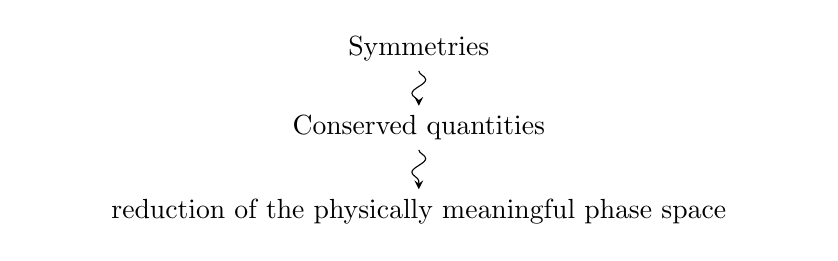
\begin{tikzpicture}[]
						\node [text width=0.8\linewidth,rectangle,align=center] (lhs) {Symmetries};
						\node [text width=0.8\linewidth, rectangle,below of=lhs,align=center] (chs) {Conserved quantities};
						\node [text width=0.8\linewidth, rectangle,below= 0.5 of chs,align=center] (rhs) {reduction of the physically meaningful phase space};
						\draw[-stealth,decorate,decoration={snake}] (lhs) -- (chs);
						\draw[-stealth,decorate,decoration={snake}] (chs) -- (rhs);
					\end{tikzpicture}						
				\end{upshotblocktitle}    	
			}
		\end{column}	
	
	\end{columns}




\end{frame}
\note[itemize]{
	\item among all possible symmetries there's a special class
	\item slogan:		Hamiltonian symmetry $\Leftrightarrow$ Admits a comoment map
	\item comomentum maps are one of the most powerful tools in the geometric mechanics toolbox
	
}
%-------------------------------------------------------------------------------------------------------------------------------------------------

%
%\begin{frame}
%						\begin{tikzpicture}
%							\pgfmathsetmacro\theta{-120}
%							\pgfmathsetmacro\viewpitch{30}
%							\pgfmathsetmacro\diam{2}
%							\pgfmathsetmacro\H{4}
%							\pgfmathsetmacro\deltaH{.5}
%							\pgfmathsetmacro\X{\diam}
%							\pgfmathsetmacro\Y{\diam*sin(\viewpitch)}	
%							\pgfmathsetmacro\vel{\diam/4}	
%													
%							
%							\draw[green,dashed,fill=green!20] (0,0) ellipse ({\X} and {\Y});
%							%\draw [blue,dashed] (-1.25,-3.5) arc (180:360:1.25 and -0.5);
%							\draw[green,dashed,fill=green!20] (0,-{\H}) ellipse ({\X} and {\Y});
%							\draw [blue,dashed] (-{\X},-{.5*\H}) arc (180:360:{\X} and -{\Y});
%		
%							\draw [green](-{\X},0) -- (-{\X},-{\H});
%							\draw [green]({\X},-{\H}) -- ({\X},0);  
%							\fill [green!80,opacity=0.5] (-{\X},0) -- (-{\X},-{\H}) arc (180:360:{\X} and {\Y}) -- ({\X},0) arc (0:180:{\X} and -{\Y});
%		
%							\draw [blue](-\X,-{.5*\H}) arc (180:360:{\X} and {\Y});
%		
%							\foreach \h in {0,-\deltaH,...,-\H}{
%								\coordinate (p) at (0,\h)++({cos(\theta)*\X},{sin(\theta)*\Y});
%								%\fill[blue] (0,\h)++({cos(\theta)*\X},{sin(\theta)*\Y}) circle(2pt);
%								\draw[red,-stealth] (0,\h)++({cos(\theta)*\X},{sin(\theta)*\Y}) --++({-\vel*sin(\theta)},{\vel*cos(\theta)*sin(\viewpitch)});
%								\draw[red] ({cos(\theta)*\X},{sin(\theta)*\Y}) -- ({cos(\theta)*\X},{sin(\theta)*\Y-\H});
%		
%						}
%		
%					    \draw[->] (5,-{\H})--(5,0) node[above] {$\dot{\Theta}$}; % ordinate
%					    \draw[->] (4,-{.5*\H})--(6,-{.5*\H})node[right] {$L$}; % ascisse
%					    \draw[-,red] (4,-{\H})--(6,0); % l'axe des abscisses
%		
%					\end{tikzpicture}		
%
%\end{frame}


\end{document}
	%+----------------------------------------------------------------------------+
%| SLIDES: 
%| Chapter: About going from symplectic to multisymplectic
%| Author: Antonio miti
%| Event: PHD preliminary Defence
%+----------------------------------------------------------------------------+


%- HandOut Flag -----------------------------------------------------------------------------------------
\makeatletter
\@ifundefined{ifHandout}{%
  \expandafter\newif\csname ifHandout\endcsname
}{}
\makeatother

%- D0cum3nt ----------------------------------------------------------------------------------------------
\documentclass[beamer,10pt]{standalone}   
%\documentclass[beamer,10pt,handout]{standalone}  \Handouttrue  

\ifHandout
	\setbeameroption{show notes} %print notes   
\fi

	
%- Packages ----------------------------------------------------------------------------------------------
\usepackage{custom-style}




%--Beamer Style-----------------------------------------------------------------------------------------------
\usetheme{toninus}
\usetikzlibrary{positioning}




%---------------------------------------------------------------------------------------------------------------------------------------------------
%- D0cum3nt ----------------------------------------------------------------------------------------------------------------------------------
\begin{document}
%------------------------------------------------------------------------------------------------


%-------------------------------------------------------------------------------------------------------------------------------------------------
\subsection{Going higher}
%-------------------------------------------------------------------------------------------------------------------------------------------------

%-------------------------------------------------------------------------------------------------------------------------------------------------
\begin{frame}[t]{Geometric Mechanics: Take Away Message}
	\begin{itemize}
		\item[•] \alert{States} are encoded by a \alert{symplectic manifold}.
		\begin{itemize}
			\item[-] Smooth manifolds arise naturally in the description of mechanical systems.
			\item[-] Constraints can be enforced intrinsically
			\item[-] Geo. Mech. yields an inherent intuition of diff. geom. structures.
		\end{itemize}
		\item<2->[•] \alert{Observables} quantities are encoded by \alert{smooth functions}.
		\begin{itemize}
			\item[-] The symplectic structure prescribe how to associate a vec. field to any observable.
			\item[-] Time evolution is obtained by integrating the flow along an Ham. v.f.
		\end{itemize}				
		\item<3->[•] \alert{Continuous symmetries} are encoded by \alert{symplectic Lie group actions}.
		\begin{itemize}
			\item[-] A relevant class of symmetries can be reconstructed from observables quantities via \emph{comomentum maps}.
			\item[-] Their importance lies in the existence of corresponding conserved quantities and the reduced description arising from them.
		\end{itemize}				
	\end{itemize}
	%Symplectic geometry is central
	\vfill
	%
	\onslide<4->{
		\begin{disclaimerbox}[we glossed on some technical details]
			\resizebox{.85\textwidth}{!}{
				\begin{columns}
					\begin{column}[T]{0.65\textwidth}
						\begin{itemize}
							\item[-] \color{black!80!white} Galilean / Special / General relativity (observer)
							\item[-] Holonomics / Non-holonomics constraints
							\item[-] Conservative / Dissipative system
							\item[-] Discrete / \alert{Continuous} degrees of freedom.
						\end{itemize}
					\end{column}					
					\begin{column}[T]{0.5\textwidth}
						\begin{itemize}
							\item[-] \color{black!80!white} Classical / Quantum observability
							\item[-] Lagrangian / Hamiltonian dynamics
							\item[-] Velocities $\neq$ Momenta
							\item[-] Local / Global flow integrability
						\end{itemize}
					\end{column}							
				\end{columns}
			}				
		\end{disclaimerbox}	
	}

\end{frame}
\note[itemize]{
	\item è centrale nel senso che è l'arena  in cui descrivere molti sistemi ideali
	\item richiede estensioni e generalizzazioni per codificare casi di studio piu' realistici e/o generali

	\item geometry is an intrisic part of mechanics. 
	The set of configurations has a natural geometric structure, constraints are automatically satisfied by this choice.
	\item {\bf descibing states as points of a manifold is the principal premise of geometric mechanics.}
	\item Conf. space and Phase space are manifolds (higher dimensional generalization of surfaces)
	\item A large class of constraints can be enforced intrinsically by the topology (shape) of the manifold.


	\item an important trait of geometric mechanics is its intuitive nature: structures and time evolution of mechanical systems can be illustrated by visualizing configuration and phase space.
	Practilly working in Geo. Mech. often means to exploit the inherent geometric intuition.
	
	\item an important characteristic is its emphasis on laying a rigourous mathematical foundation on which one can build upon mechanics. 
	While Newtonian mechanics is highly desciptive it does not reveal the underlying structure.
	In geo. mech. computations are structural arguments which provide insight into the frabic they represent. 

	\item Huge disclaimer, in the above presentation we glossed out on many details...

}

%-------------------------------------------------------------------------------------------------------------------------------------------------




%-------------------------------------------------------------------------------------------------------------------------------------------------
\begin{frame}[t,fragile]{Multisymplectic geometry in a nutshell}
	\begin{block}{Historical motivation}
		Mechanics: geometrical foundations of \textit{(first-order)} field theories.
	\end{block}
	\vfill	
	\begin{table}
		\only<2->{
		\begin{tabular}{|p{0.2\textwidth}|p{0.3\textwidth}|p{0.35\textwidth}|} 
            \hline
            \parbox[][20pt][c]{0.2\textwidth}{mechanics} & \multicolumn{2}{c|}{geometry} \\
            \hline
            \parbox[][20pt][c]{0.2\textwidth}{phase space} & symplectic manifold & \only<3->{multisymplectic manifold} \\[.25em]
            \parbox[][20pt][c]{0.2\textwidth}{classical \\ observables} & Poisson algebra & \only<3->{$L_\infty$-algebra} \\[.25em]
            \parbox[][20pt][c]{0.2\textwidth}{symmetries} &  group actions admitting comoment map & 
            \only<3->{group actions admitting 
				\tikz[baseline,remember picture]{\node[rounded corners,
	                        fill=orange!10,draw=orange!30,anchor=base]            
	            			(target) {homotopy comomentum map};
	            }
            }
            \\
            \hline
  \multicolumn{1}{c}{}
            &  
            \multicolumn{1}{@{}c@{}}{$\underbrace{\hspace*{.3\textwidth}}_{\text{point-like particles systems}}$} 
            &
            \multicolumn{1}{@{}c@{}}{\only<4->{$\underbrace{\hspace*{.3\textwidth}}_{\text{field-theoretic systems}}$}} 
		\end{tabular}
		}
	\end{table}		
	\vfill
	\onslide<4->{
		\begin{block}{Scope of the thesis}
			\begin{itemize}
				\item[$\bullet$] Develop theory of 
					\tikz[baseline,remember picture]{\node[rounded corners,
	                        fill=orange!10,draw=orange!30,anchor=base]            
	            			(base) {homotopy comomentum maps};
	            	}
	            \item[$\bullet$] produce new meaningful examples.
			\end{itemize}
		\end{block}
		%
        \begin{tikzpicture}[overlay,remember picture]
			\path[->]<4-> (base.east) edge[bend right](target.south east);
		\end{tikzpicture}
	}
	%
\end{frame}
\note[itemize]{
	\item Historically, the interest in multisymplectic manifolds, has been motivated by the need for understanding the geometrical foundations of first-order classical field theories.
	The key point is that, just as one can associate a symplectic manifold to an ordinary classical mechanical system (e.g. a single
point-like particle constrained to some manifold), it is possible to associate a multisymplectic
manifold to any classical field system (e.g. a continuous medium like a filament or a fluid). See frame Extra-\ref{Frame:Ms-Field-Mechanics} 
	
	\item General ideas basic parallelisms with caveats
	\item caveat: points in multiphase spaces are not states
	\item the table hides the duality between geometric and algebraic approaches to the problem.
	\item 
}
%-------------------------------------------------------------------------------------------------------------------------------------------------












%----------------------------------------------------------------------------------------------------------------------------------
\end{document}
%----------------------------------------------------------------------------------------------------------------------------------











%-------------------------------------------------------------------------------------------------------------------------------------------------
\section{Technical Background}
	\checkpoint
	%+----------------------------------------------------------------------------+
%| SLIDES: 
%| Chapter: Brief introduction to multisymplectic geometry and Homotopy momap
%| Author: Antonio miti
%| Event: PHD preliminary Defence
%+----------------------------------------------------------------------------+

%- HandOut Flag -----------------------------------------------------------------------------------------
\newif\ifHandout

%- D0cum3nt ----------------------------------------------------------------------------------------------
\documentclass[beamer,10pt]{standalone}   
%\documentclass[beamer,10pt,handout]{standalone}  \Handouttrue  

%- HandOut Flag -----------------------------------------------------------------------------------------
\ifHandout
	\setbeameroption{show notes} %print notes   
\fi

	
%- Packages ----------------------------------------------------------------------------------------------
\usepackage{custom-style}


%--Beamer Style-----------------------------------------------------------------------------------------------
\usetheme{toninus}





%---------------------------------------------------------------------------------------------------------------------------------------------------
%- D0cum3nt ----------------------------------------------------------------------------------------------------------------------------------
\begin{document}
%------------------------------------------------------------------------------------------------






%-------------------------------------------------------------------------------------------------------------------------------------------------
\subsection{Multisymplectic geometry}
%-------------------------------------------------------------------------------------------------------------------------------------------------





%-------------------------------------------------------------------------------------------------------------------------------------------------
\begin{frame}[fragile]{Multisymplectic manifolds} %Fragile -->workaround tikzcd
	\begin{defblock}[$n$-plectic manifold ~\emph{(Cantrijn, Ibort, De Le\'on)}]
	\includestandalone[width=0.95\textwidth]{Pictures/Figure_multisym}	
	\end{defblock}
	%
	\begin{defblock}[Non-degenerate $(n+1)$-form]
		\begin{columns}
			\begin{column}{.45\linewidth}
				\centering{
				The $\omega^\flat$ (flat) bundle map is injective.
				}
			\end{column}
			\begin{column}{.5\linewidth}
						\vspace{-.5em}
				\[
				\begin{tikzcd}[column sep= small,row sep=0ex,
				/tikz/column 1/.append style={anchor=base east}]
				    \omega^\flat \colon T M \ar[r]& \Lambda^n T^\ast M \\
  						 (x,u) \ar[r, mapsto]& (x,\iota_{u} \omega_x)						
				\end{tikzcd}	
				\]
			\end{column}
		\end{columns}
	\end{defblock}
	%
	\pause
	\begin{defblock}[Hamiltonian $(n-1)$-forms]
		\begin{displaymath}
			\Omega^{n-1}_{ham}(M,\omega) 	:=
			\biggr\{ \sigma \in  \Omega^{n-1}(M) \; \biggr\vert \; 
				\exists \mathscr{v}_\sigma \in \mathfrak{X}(M) ~:~ 
				\tikz[baseline,remember picture]{\node[rounded corners,
                        fill=orange!5,draw=orange!30,anchor=base]            
            			(target) {$d \sigma = -\iota_{\mathscr{v}_\sigma} \omega$ };
            	}				
				~\biggr\} 
			\end{displaymath}
	\end{defblock}
	%
	%
	\pause
		\tikz[overlay,remember picture]
		{
			\node[rounded corners,
                 fill=orange!5,draw=orange!30,anchor=base]            
            	 (base) at ($(current page.east)-(2.25,1.8)$) [rotate=-0,text width=4cm,align=center] {\footnotesize{\textcolor{red}{Hamilton-DeDonder-Weyl \\equation}}};
		}	
	\begin{tikzpicture}[overlay,remember picture]
    	\path[->] (base.west) edge[bend left,red](target.south west);
    \end{tikzpicture}	
	\pause
	\vfill
	%
	\begin{block}{Examples:}
		\vspace{-.5em}
		\setbeamercovered{transparent}
		\begin{itemize}[<+->]
			\item[$\bullet$] $n=1$ \qquad\qquad\qquad $\Rightarrow$\quad $\omega$ is a symplectic form
			\item[$\bullet$]  $n=(dim(M)-1)$ \quad$\Rightarrow$\quad $\omega$ is a volume form
			%Any oriented $(n+1)$-dimensional manifold is $n$-plectic w.r.t. the volume form.
			%\item[$\bullet$] Let $G$ a semisimple Lie group and $\langle\cdot,\cdot \rangle$  its killing form. Then $\langle [\cdot,\cdot],\cdot \rangle$ extends to a biinvariant multisymplectic form $\omega$.
			\item[$\bullet$] Let $Q$ a smooth manifold, the multicotangent bundle $\Lambda^n T^\ast Q$ is naturally $n$-plectic.%
			\quad
			\textit{(cfr, \href{https://arxiv.org/abs/physics/9801019}{GIMMSY} construction for classical field theories)}
		\end{itemize}
	\end{block}			 
	
%
\end{frame}
\note[itemize]{
	\item Multisymplectic ($n$-plectic) geometry is a generalization of symplectic geometry where a closed, non degenerate $n+1$-form $(n\geq 1)$  takes the place of the symplectic 2-form
	
	\item multisymplectic means \emph{going higher} in the degree of $\omega$
	
	\item non degeneracy means $\iota_v\omega = 0 \Leftrightarrow v=0$.
	
	\item examples 
		\begin{itemize}
			\item[$\bullet$] 1-plectic $=$ symplectic
			\item[$\bullet$] Any oriented $(n+1)$-dimensional manifold is $n$-plectic w.r.t. the volume form.
			\item[$\bullet$] The multicotangent bundle $\Lambda^n T^\ast Q$ is naturally $n$-plectic.
		\end{itemize}
	
	\item We recognize the special class of forms, called Hamiltonian, determining the Hamiltonian vector fields. 
	Not every $n-1$ form admits an Hamiltonian vector field.
	When it exists, non degeneracy guarantees unicity.
	
	\item Observe also that, by degree reason, when $n$ is equal to $1$ or $dim(M)+1$ an injective flat map $\flat$ is also bijective.
	
	\item It is important to stress that mechanical systems are not the only source instances of this class of of structures. 
				e.g. any semisimple Lie groups has associated a 2-plectic structure and any oriented $n+1$ dimensional manifold is naturally $n$-plectic.
				

}
%---------------------------------------------------------------------------------------------------------------------------------------------------








%---------------------------------------------------------------------------------------------------------------------------------------------------
\subsection{Lie $\infty$-algebra of Observables}
\begin{frame}[fragile,t]{Lie $\infty$-algebra of Observables (higher observables) }
	Let be $(M,\omega)$ a $n$-plectic manifold.
	\begin{defblock}[$L_\infty$-algebra of observables ~\emph{(Rogers)}]
		\hspace{.25em} Is a cochain-complex $(L,\{\cdot\}_1)$ \\
		\vspace{-2.5em}
		\begin{center}
		\ifHandout
			\includestandalone{Pictures/Figure_Observables}	
		\else
			\includestandalone{Pictures/Frame_Observables}
		\fi				
		\end{center}
		\onslide<2->{
			\hspace{.25em} with $n$ (skew-symmetric) multibrackets $(2 \leq k \leq n+1)$\\
			\vspace{-1.5em}
			\begin{center}
				\includestandalone{Pictures/Equation_Multibracket}	
			\end{center}
		}
		%
	\end{defblock}
  	\vfill
	\onslide<3->{
		\emph{Higher analogue} of the \emph{Poisson algebra structure} associated to a symplectic mfd.
	\vfill
	\begin{columns}
		\hfill
		\begin{column}{.11\linewidth}	
			If $n>1$:
			
		\end{column}	
		\begin{column}{.8\linewidth}
		\begin{itemize}
			\item[\xmark] \textcolor{red}{we lose} :\quad multiplication of observables, Jacobi equation;
			%\\ \hspace*{4.25em} full-fledged Jacobi equation;
			\item[\cmark] \textcolor{green}{we gain} :\quad brackets with arities different than two,\\
			\hspace*{4.25em}
			 Jacobi equation \emph{up to homotopies}.
		\end{itemize}		
		\end{column}		
	\end{columns}
	}
  \end{frame}
 \note[itemize]{
	\item if symplectic manifolds are the symmetric take on mechanics, Poisson algebras are the algebraic counterpart.
 	\item A Lie algebra is associated to an ordinary symplectic manifold (its Poisson algebra).
	%(Underlying this is a Lie algebra, whose Lie bracket is the Poisson bracket.)
	Similarly, one associates an Lie-$n$ algebra to any $n$-plectic manifold.
 	% https://ncatlab.org/nlab/show/n-plectic+geometry 	 
 	 %https://ncatlab.org/nlab/show/Poisson+bracket+Lie+n-algebra
	 \item Basically, the higher observables algebra is a chunk of the de Rham complex of $M$ with inverted grading( convention employed here) and an extra structure called "multibrackets".
 	\item ( In the 1-plectic case it reduces to the corresponding Poisson algebra of classical observables)
 	\item Rogers associated to any n-plectic mfd a $L\-\infty$ algebra, Zambon generalized it to the pre-n-plectic case.
 	\item Recognize in the definition of $\{\cdot,\ldots,\cdot\}_k$ the contraction with hamiltonian fields $v_\sigma$ w.r.t. $\sigma$.
  	\item Note $	\iota_{v_{\sigma_1}}\cdots\iota_{v_{\sigma_k}} = (-)^{(k-1)+(k-2)+\dots+1}\iota_{v_{\sigma_k}}\cdots\iota_{v_{\sigma_1}} = (-)^{\frac{k(k-1)}{2}}\iota_{v_{\sigma_k}}\cdots\iota_{v_{\sigma_1}}$ 
 	The definition usually find in literature of Rogers multibrackets involves the coefficient $ (-)^{\frac{k(k-1)}{2}} = -\varsigma(k-1) = (-)^{k+1} \varsigma(k)$.
  \item higher observables is Special instance of a more general object  called $L\-\infty$ Algebra...
 }
%------------------------------------------------------------------------------------------------


%-------------------------------------------------------------------------------------------------------------------------------------------------
\subsection{Homotopy comomentum maps}\label{frame:hcmm-main}
\begin{frame}[fragile]{Homotopy comomentum maps}
	Consider a Lie algebra action $v:\mathfrak{g} \to \mathfrak{X}(M)$  \underline{preserving the $n$-plectic form $\omega$}.
	\vfill
	\begin{defblock}[Homotopy comomentum map \emph{(Callies, Fregier, Rogers, Zambon)}]
		\ifHandout
			\includestandalone{Pictures/Figure_Lifting}
		\else
			\includestandalone{Pictures/Frame_Lifting}
		\fi					
	\end{defblock}
	\onslide<4->{
	\begin{lemblock}[HCMM unfolded  \cite{Callies2016}]
			%
			HCMM is a sequence of (graded-skew) multilinear maps:
			\begin{displaymath}
				(f)  = \big\lbrace f_k: \; \Lambda^k{\mathfrak g} \to L^{1-k} \subseteq \Omega^{n-k}(M) 
				~\big\vert~ 0\leq k \leq n+1  \big\rbrace
			\end{displaymath}
			\emph{fulfilling:}%\emph{such that:}
			\begin{itemize}
				\item<5-> $f_0 = 0 $, $f_{n+1} = 0$
				\item<6-> $d f_k (p) = f_{k-1} (
				\tikz[baseline,remember picture]{\node[rounded corners,
                        fill=green!5,draw=green!30,anchor=base]            
            			(target) {$\partial $ };
            	}				
				p)  - (-1)^{\frac{k(k+1)}{2}} \iota(v_p) \omega 
				\qquad\scriptstyle \forall p \in \Lambda^k(\mathfrak{g}),\; \forall k=1,\dots n+1$
			\end{itemize}
		\onslide<7->{
			\tikz[overlay,remember picture]
			{
				\node[rounded corners,
	                 draw=green!30,anchor=base]            
	            	 (base) at ($(current page.east)-(3,3)$) [rotate=-0,align=center] {\footnotesize{\hyperlink{frame:CE-complex}{\emph{Chevalley-Eilenberg boundary op.}}}};
			}	
		\begin{tikzpicture}[overlay,remember picture]
	    	\path[->] (base.west) edge[bend right,green](target.north east);
	    \end{tikzpicture}
	    }
	\end{lemblock}	
	}
	\vfill
\end{frame}
\note[itemize]{
	\item  An infinitesimal symmetry is a lie algebra morphism such that $\mathcal{L}_{v_x} \omega = 0 ~ \forall x \in \mathfrak{g}$.
	\\ (It is also call an infinitesimal multisymplectic action and $v_x$ is the infinitesimal generator of the action, corresponding to $x \in \mathfrak g$.) 
	\item Essentially, admitting a comoment maps mean that $v$ acts via Hamiltonian vector fields.
	\item In mechanical terms, a moment map is a tool associated with a Hamiltonian action of a Lie group on a symplectic manifold, used to construct conserved quantities for the action.(see \ref{frame:HCMMandConserved} in appendix.
}
%-------------------------------------------------------------------------------------------------------------------------------------------------








%----------------------------------------------------------------------------------------------------------------------------------
\end{document}
%----------------------------------------------------------------------------------------------------------------------------------





%-------------------------------------------------------------------------------------------------------------------------------------------------



%-------------------------------------------------------------------------------------------------------------------------------------------------
\section{Foreground}
%-------------------------------------------------------------------------------------------------------------------------------------------------

%-------------------------------------------------------------------------------------------------------------------------------------------------
	\subsection{Hydrodynamical homotopy moment map and Knots}
	\subcheckpoint	
	%+----------------------------------------------------------------------------+
%| SLIDES: 
%| Chapter: Results of the paper with M. Spera
%| Author: Antonio miti
%| Event: PHD preliminary Defence
%+----------------------------------------------------------------------------+

%- HandOut Flag -----------------------------------------------------------------------------------------
\newif\ifHandout

%- D0cum3nt ----------------------------------------------------------------------------------------------
\documentclass[beamer,10pt]{standalone}   
%\documentclass[beamer,10pt,handout]{standalone}  \Handouttrue  

%- HandOut Flag -----------------------------------------------------------------------------------------
\ifHandout
	\setbeameroption{show notes} %print notes   
\fi
	
%- Packages ----------------------------------------------------------------------------------------------
\usepackage{custom-style}

%--Beamer Style-----------------------------------------------------------------------------------------------
\usetheme{toninus}



%---------------------------------------------------------------------------------------------------------------------------------------------------
%- D0cum3nt ----------------------------------------------------------------------------------------------------------------------------------
\begin{document}
%------------------------------------------------------------------------------------------------


\begin{frame}{Applications to hydrodynamics and knot theory}\label{frame:hydro1}
	\begin{columns}[T] % align columns
	\begin{column}{.4\textwidth}
		\vspace{.5em}
		\centering
			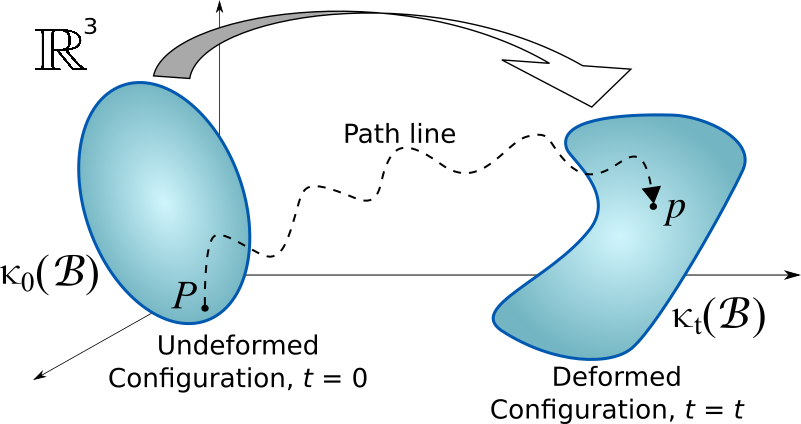
\includegraphics[width=\linewidth]{Pictures/Figure_continuum}
	\end{column}
	%
	\hfill
	%
	\begin{column}{.6\textwidth}
		\scalebox{.8}{%
			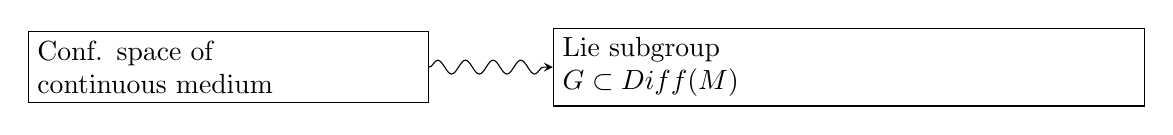
\begin{tikzpicture}[
				node distance=0.65\linewidth,
				]
				\node [text width=0.4\linewidth,rectangle,draw] (lhs) {Conf. space of\\ continuous medium};
				\node [text width=0.6\linewidth, rectangle,draw,right of=lhs] (rhs) {Lie subgroup \\$G \subset Diff(M)$};
				\draw[-stealth,decorate,decoration={snake}] (lhs) -- (rhs);
			\end{tikzpicture}
		}		
		Examples:
		\scalebox{.8}{%		
		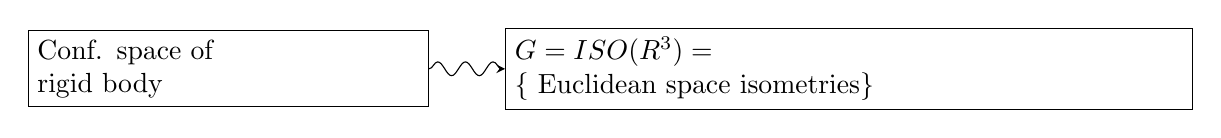
\begin{tikzpicture}[
			node distance=0.65\linewidth,
			]
			\node [text width=0.4\linewidth,rectangle,draw] (lhs) {Conf. space of\\ rigid body};
			\node [text width=0.7\linewidth,rectangle,draw,right of=lhs] (rhs) {$G=ISO(\mathbb{R}^3)=$\\ $\{$
				Euclidean space isometries$\}$};
			\draw[-stealth,decorate,decoration={snake}] (lhs) -- (rhs);
		\end{tikzpicture}
		}
		\scalebox{.8}{%
		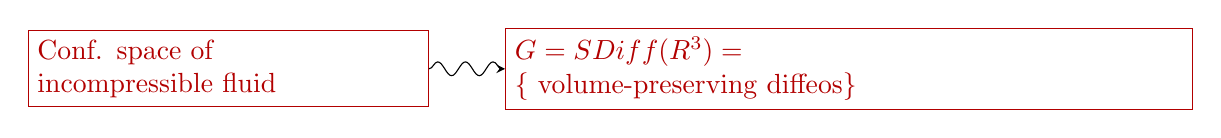
\begin{tikzpicture}[
			node distance=0.65\linewidth,
			]
			\node [text width=0.4\linewidth,red!70!black,rectangle,draw] (lhs) {Conf. space of\\ incompressible fluid};
			\node [text width=0.7\linewidth,red!70!black,rectangle,draw,right of=lhs] (rhs) {$G= SDiff(\mathbb{R}^3)=$\\ $\{$
				volume-preserving diffeos$\}$};
			\draw[-stealth,decorate,decoration={snake}] (lhs) -- (rhs);
		\end{tikzpicture}
		}
	\end{column}%
	\end{columns}
	\pause
	\vfill
	We consider the following setting:
	
	\begin{itemize}%[<+->]
		\item[$\bullet$]2-plectic manifold: 
		\vspace{-1em} 
			$$M=(\mathbb{R}^3,\nu = dx\wedge dy\wedge dz)$$
			\vspace{-.8em}\pause
		\item[$\bullet$]$\infty$-dim. Lie algebra (\emph{ideal fluid velocities}): \vspace{-1em}
			$$\mathfrak{g}:= sdiff_0(\mathbb{R}^3) = \left\lbrace  X \in \mathfrak{X}(\mathbb{R}^3) ~\left\vert~ 
		  		\substack{ div X = 0, \\ \textrm{\emph{ rapidly vanishing at }}\infty} \right\rbrace \right.$$
		  	\vspace{.2em}\pause
		\item[$\bullet$] Multisymplectic Lie algebra action:
			\vspace{-1em} 
			$$\mathfrak{g}= sdiff_0 \hookrightarrow  \mathfrak{X}(\mathbb{R}^3)$$
\end{itemize}		
	\pause
	\vfill
	\begin{center}
	\tcbox[enhanced,frame hidden,borderline={0.5pt}{0pt}{red,dashed}]{	
		\alert{
		\faQuestionCircle \qquad
			{Does $sdiff_0 \circlearrowleft (\mathbb{R}^3,\nu = dx\wedge dy\wedge dz)$ admit an HCMM?}	
		\qquad \faQuestionCircle		
		}
	}
	\end{center}

\end{frame}
\note[itemize]{
	\item We are working in the setting of \emph{geometric continuum mechanics} .\\
		Recall that the configuration space of a continuum object is encoded via diffeomorphisms. In the case of an incompressible fluid is encoded via volume-preserving diffeomorphisms.
	\item (Configution space is the set of spatial displacement of a mechanical systems. These are different from the \emph{physical states}.
	\item Such manifolds are infinite dimensional. Particular caution has to be taken in defining the smooth structure in this case.
	\item However, what really matters in the construction of a moment map is the infinitesimal action, i.e. the Lie algebra. In our case, the infinitesimal action to be considered is via divergence-free vector fields.
	\item (Notation): In the following M will be the 3 dimensional Euclidean Space.
	\item The simple but crucial observation is that the standard volume form on the euclidean space is a multisymplectic form.


}



%---------------------------------------------------------------------------------------------------------------------------------------------------
\begin{frame}{A Hydrodynamical HCMM}\label{frame:hydro2}
	\begin{columns}
		\begin{column}[c]{.5\linewidth}
		  	\begin{itemize}
		  		\item The observables are  $$L= \Omega^1_{\textrm{ham}}(\mathbb{R}^3)\oplus\Omega^0(\mathbb{R}^3)$$
		  		\item \hyperlink{frame:hydromomap-details}{HCMM consists of a pair of functions}:
					\begin{align*}
						f_1 &\colon \mathfrak{g} \rightarrow \Omega^1_{\textrm{ham}}(\mathbb{R}^3) \\
						f_2 &\colon \mathfrak{g}\wedge\mathfrak{g} \rightarrow C^\infty(\mathbb{R}^3)
					\end{align*}	
		  	\end{itemize}
		\end{column}	
	  	\hfill  	
		\begin{column}[c]{.5\linewidth}
  		\includestandalone[width=\textwidth]{Pictures/Figure_Euclid_Trigger}
 	 	\end{column}
 	 \end{columns}


	\pause
\tcbset{colback=white,
	colbacktitle=white,
	colframe=blue!70!black,
	boxrule=1pt,
	colupper=blue!70!black,
	arc=15pt,
	}
	\begin{tcolorbox}[sidebyside,righthand width=.75\linewidth]
		Thm: \cite{Miti2018}
		\tcblower
		\vspace{-1.5em}
		\begin{columns}
		\begin{column}{.6\linewidth}	
		\begin{align*}
		f_1 &= \flat \circ \text{curl}^{-1} 
		%~:~ \mathfrak{g} \to \Omega^{1}_{Ham}(\mathbb{R}^3)
		%\qquad \text{\small ("Biot-Savart law")}
		%\tag{\small"Biot-Savart law"}
		\\
		f_2 &= \Delta^{-1} \circ \delta \circ (f_1 \circ \partial_{CE} +\iota(\cdot)\omega) 
		%~:~ \wedge^2\mathfrak{g} \to C^{\infty}(\mathbb{R}^3)
		%\tag{\small"Coulomb law"}
		\end{align*}		
		\end{column}	
		\begin{column}{.5\linewidth}
			\begin{center}
				\tikz[baseline,remember picture]{\node[rounded corners,
                        fill=orange!5,draw=orange!30,anchor=base]            
            			(base) [rotate=-0,text width=3cm,align=left]{
            				\hyperlink{frame:RiemannianGeneralization}{
            					\footnotesize{
            					Riemannian structure\\\quad plays a crucial role
							}            				
            				}
            			};
            	}		
			\end{center}					
		\end{column}			
		\end{columns}	
	\end{tcolorbox}
	\pause
	\vfill
	\hyperlink{frame:hydro-reinterpretation}{Getting back to hydrodynamics}:
	\begin{tcolorbox}[sidebyside,righthand width=.75\linewidth]
		Thm: \cite{Miti2018}
		\tcblower
		HCMM for $G\circlearrowright(\mathbb{R}^3,\nu)$ induces an ordinary co-mo.map for $G\circlearrowright (LS,\nu^{\ell})$ via \emph{trasgression.}
		\\[.5em]
		\hyperlink{frame:HydroHCMM-reinterpretation}{\alert{\small\emph{(Arnol'd-Marsden-Weinstein hydrodynamical co-momentum map)}}}
		\vfill			
	\end{tcolorbox}


\end{frame}
\note[itemize]{
	\item relation with knot theory: looking at the knot as a fluid configuration with singular vorticity along a knotted tube,
	\item subalgebra of the infinitesimal action of $SDiff(\mathbb{R}^3)$
	\item observe how elements from Riemannian geometry and hodge theory appear in the construction
		\begin{itemize}
			\item $\delta$ codifferential
			\item $\Delta$ Laplacian
			\item $\flat$ $\sharp$  musical isomorphisms
		\end{itemize}

	\item
	Applications:
	\begin{itemize}[<+->]%[<alert@+>]
		\item[\CheckedBox]  Hydrodynamics interpretation: Rasetti-Regge currents as "momenta".
		% is exhibited upon resorting to the Euler equation for perfect fluids.
		\item[\CheckedBox]  Knot theory: reinterpretation of the (Massey) higher order linking numbers in terms of conserved quantities.
		\item[\CheckedBox]  Semiclassical interpretation of the HOMFLYPT polynomial.
	\end{itemize}

	\item other results of the paper: 	
	\begin{itemize}
		\item[\CheckedBox]  Explicit construction of an HCMM for $SDiff_0 \circlearrowright (\mathbb{R}^3,\nu)$ (and generalization to Riemannian homological spheres);
		\item[\CheckedBox]  Hydrodynamics interpretation: proved that this HCMM trasgresses to the standard hydrodynamical co-momentum map of  Arnol'd, Marsden and Weinstein and others; (we recover a quantitity already in use in mechanics)
		% is exhibited upon resorting to the Euler equation for perfect fluids.
		\item[\CheckedBox]  Application to knot theory: reinterpretation of the (Massey) higher order linking numbers in terms of conserved quantities and determined the knot theoretic analogues of first integrals in involution.



	\end{itemize}
	
}
%---------------------------------------------------------------------------------------------------------------------------------------------------



%---------------------------------------------------------------------------------------------------------------------------------------------------
  \begin{frame}{Knot differential forms as observables}\label{frame:hydro3}
	IDEA: Vortex theory approach to knots:
	\begin{itemize}
		\item[\xmark] knots as embeddings $S^1\hookrightarrow \mathbb{R}^3$.
		\item[\cmark] knots as ideal fluid configurations with vorticity concentrated on closed curves
	\end{itemize}
	\pause
	%
	\vfill
  	\begin{columns}
		\begin{column}[c]{.7\linewidth}	
				Let $ L = \cup_{i=1}^n L_i$ be an oriented link in ${\mathbb R}^3$ 
				\\(components $L_i$, $i=1,\dots,n$ required to be  {\it trivial} knots)	
		\end{column}
		\begin{column}[c]{.25\linewidth}
			\centering{
			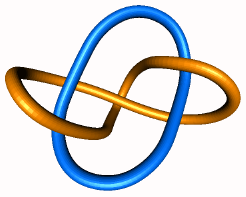
\includegraphics[width=0.75\linewidth]{./Pictures/Whiteheadlink}
			}
		\end{column}
  	\end{columns}
	%
	\pause
  	\begin{columns}
		\begin{column}[t]{.5\linewidth}	
			\begin{defblock}[Vorticity 2-form]
				$$
				\omega_{L} := \sum_{i=1}^n \omega_{L_i}, \qquad d\omega_L = 0
				$$
				($\omega_{ L_i}$ = \hyperlink{frame:poinduals}{Poincar\'e dual} associated to $L_i$)
			\end{defblock}
		\end{column}
		\begin{column}[t]{.5\linewidth}	
			\begin{defblock}[Velocity 1-form]
				\vspace{-.75em}
				$$
 					v_{ L} = \sum_{i=1}^n v_{L_i}, \qquad \qquad  dv_{L} = \omega_{ L}
				$$
				($v_{L_i} := \omega_{{\mathfrak a}_i}$ = \hyperlink{frame:poinduals}{Poincar\'e dual}  of a disc ${\mathfrak a}_i$ 
				bounded by 	$L_i$ \footnotesize{(Seifert surface)}) 
			\end{defblock}						
		\end{column}
  	\end{columns}
	%
	\pause
	%
	\tcbset{colback=white,
	colbacktitle=white,
	colframe=blue!70!black,
	boxrule=1pt,
	colupper=blue!70!black,
	arc=15pt,
	}
	\begin{tcolorbox}[sidebyside,righthand width=.7\linewidth]
		Thm: \cite{Miti2018}
		\tcblower
		$v_{L}$ is a {\it Hamiltonian 1-form}
		\\[.5em]
		\pause
		\hyperlink{frame:highorderlinking}{\footnotesize{(the same applies to every \emph{"higher velocity $1-form$})}}.
	\end{tcolorbox}	
	 

  
  \end{frame}
  \note[itemize]{
  	\item $G~=~SDiff_0(\mathbb{R}^3)$	(volume-preserving diffeomorphisms) encompasses ambient isotopies of knotted links (interpreted as singular vortices) and Euler evolution
	\item "instead as considering the knot we focus on its complementary"
	\item the context allows to understand certain knot theoretic quantities as hamiltonian forms
	\item $\omega_{ L_i}$ denote the Poincar\'e (or Thom) dual (class) associated to $L_i$: they are 2-forms localized in a 
 cross-section of a  suitable tubular neighbourhood $T_i$ around $L_i$ - with total fibre integral equal to one, or, as currents, 2-forms which are $\delta$-like on $L_i$
 
	\item $v_{L_i} := \omega_{{\mathfrak a}_i}$ is the Poincar\'e dual (class) of a disc ${\mathfrak a}_i$ bounding
$L_i$ (a Seifert surface for the trivial knot $L_i$). Precisely:
$$
\partial {\mathfrak a}_i = L_i, \qquad \qquad dv_{L_i} = d\omega_{{\mathfrak a}_i} = \omega_{L_i} = \omega_{\partial {\mathfrak a}_i},
$$
	\item
		Velocity 1-forms $v_i$ correspond (upon approximation of the associated Euler equation) to the so-called LIA (Linear Induction Approximation) or  {\it binormal evolution}
		of the ``vortex ring" $L_i$ (``orthogonal" to the discs ${\mathfrak a}_i$.
		
	\item Everything is up to choices of tubular neighbourhoods, Seifert surface and specific Poincar\'e dual.	
	
}
%------------------------------------------------------------------------------------------------





%----------------------------------------------------------------------------------------------------------------------------------
\end{document}
%----------------------------------------------------------------------------------------------------------------------------------

%-------------------------------------------------------------------------------------------------------------------------------------------------
%-------------------------------------------------------------------------------------------------------------------------------------------------
	\subsection{Multisymplectic compact group actions on spheres}
	\subcheckpoint	
	%+----------------------------------------------------------------------------+
%| SLIDES: 
%| Chapter: Results of the paper with L. Ryvkin
%| Author: Antonio miti
%| Event: PHD preliminary Defence
%+----------------------------------------------------------------------------+

%- HandOut Flag -----------------------------------------------------------------------------------------
\newif\ifHandout

%- D0cum3nt ----------------------------------------------------------------------------------------------
\documentclass[beamer,10pt]{standalone}   
%\documentclass[beamer,10pt,handout]{standalone}  \Handouttrue  

%- HandOut Flag -----------------------------------------------------------------------------------------
\ifHandout
	\setbeameroption{show notes} %print notes   
\fi

	
%- Packages ----------------------------------------------------------------------------------------------
\usepackage{custom-style}

%--Beamer Style-----------------------------------------------------------------------------------------------
\usetheme{toninus}




\renewcommand{\action}{\circlearrowleft}

\newcommand*{\TakeFourierOrnament}[1]{{%
\fontencoding{U}\fontfamily{futs}\selectfont\char#1}}
\newcommand*{\danger}{\TakeFourierOrnament{66}}







%---------------------------------------------------------------------------------------------------------------------------------------------------
%- D0cum3nt ----------------------------------------------------------------------------------------------------------------------------------
\begin{document}
%------------------------------------------------------------------------------------------------

%-------------------------------------------------------------------------------------------------------------------------------------------------
\begin{frame}[fragile]{Problem: Geometric interpretation of cohomological obstructions}\label{frame:introcohoobstruction}
	Given a multisymplectic group action $\vartheta:G\action (M,\omega)$ 
	
	How to determine if $\vartheta$ admits a HCMM?
	
	\vfill
	\begin{tcolorbox}
		$\exists$ auxiliary complex encoding a HCMM
		\begin{displaymath}
			C_{\mathfrak{g}} := CE(\mathfrak{g})\otimes \Omega(M) = 
			\text{tot}\Big(\Lambda^{\geq 1} 
		\mathfrak{g}^*\otimes \Omega^\bullet(M),~ \delta_\text{CE},~d~\Big)
		\end{displaymath}
	\end{tcolorbox}

		HCMM are in 1:1 with primitives of a certain cocycle \hyperlink{frame:AppCohomoObstructions}{(constructed out of $\omega$ and $v$)}
	%
	\pause
	
\tcbset{colback=white,
	colbacktitle=white,
	colframe=blue!70!black,
	boxrule=1pt,
	colupper=blue!70!black,
	arc=15pt,
	}
\begin{tcolorbox}[sidebyside,righthand width=7cm]
	Prop: \cite{Ryvkin2015}+\cite{Fregier2015}
\tcblower
	$\exists$ HCMM 
	$\Leftrightarrow ~ \lbrack\tilde{\omega}\rbrack=0\in H^{n+1}(C_\mathfrak g)$
\end{tcolorbox}

	\pause
	\vfill
	Disadvantages:
	\begin{itemize}
		\item \danger purely algebraic \danger
		\item Desirable to translate it in a cohomology theory pertaining to the geometrical data.
	\end{itemize}


\end{frame}
\note[itemize]{
	\item idea: 	
		A HCMM is a sequence of multilinear maps $f_k \in Hom(\wedge^k \mathfrak{g},\Omega^{n-k}(M))\subset C_\mathfrak{g}^n$
	\item
		
	\item equivariant cohomology = "cohomology theory applying to topological spaces with group actions"

}
%-------------------------------------------------------------------------------------------------------------------------------------------------


%-------------------------------------------------------------------------------------------------------------------------------------------------
\begin{frame}[fragile]{Cohomological obstructions for compact groups}\label{frame:obstructioncompactgroups}
\tcbset{colback=white,
	colbacktitle=white,
	colframe=blue!70!black,
	boxrule=1pt,
	colupper=blue!70!black,
	arc=15pt,
	}
\begin{tcolorbox}[sidebyside,righthand width=7cm]
	Prop: \cite{Callies2016}+\cite{Fregier2015}
\tcblower
	Translation of $[\tilde{\omega}]$ in terms of the \emph{Bott-Shulman-Stasheff} and \emph{Cartan} models of 
	\tikz[baseline,remember picture]{\node[rounded corners,
                        fill=orange!10,draw=orange!30,anchor=base]            
            			(target) {\hyperlink{frame:EquivariantCohomology}{equivariant cohomology}};
            	}					
\end{tcolorbox}
	\pause
		\tikz[overlay,remember picture]
		{
			\node[rounded corners,
                 fill=orange!10,draw=orange!30,anchor=base]            
            	 (base) at ($(current page.north east)-(2.25,3.25)$) [rotate=-0,text width=4cm,align=center] {\footnotesize{cohomology theory for group actions on topological spaces}};
		}	
	\begin{tikzpicture}[overlay,remember picture]
    	\path[->] (base.north) edge[bend right,red](target.east);
    \end{tikzpicture}	

	\pause	
	\vfill
	Disadvantages:
	\begin{itemize}
		\item difficult to compute
		\item dependent on the models.
	\end{itemize}
	\pause

	\begin{tcolorbox}[
		enhanced,frame hidden,
		borderline={0.5pt}{0pt}{purple!70!black,dashed},
		sidebyside,righthand width=9cm,colframe=purple!70!black]	
	\alert{Goal:}
	\tcblower
	 Read obstructions in a simpler (more geometrical) cohomology theory (at least in simpler cases)
	\end{tcolorbox}
	\pause
	\vfill
	\vspace{1em}
	Let $\vartheta:G\times M\to M$ be a compact Lie group action:
	\begin{thmblock}[\cite{Miti2019}]
	\hyperlink{frame:cohomologicalproposition}{
	\vspace{-1em}
	$$\vartheta ~\text{admits HCMM}~ ~\Longleftrightarrow~  
	 ~[\vartheta^*\omega-\pi^*\omega]=0\in H^{n+1}_{dR}(G\times M)$$ 
	 }
	 \vspace{-1.5em}
	\end{thmblock}


\end{frame}
\note[itemize]{

	
	\item equivariant cohomology = "cohomology theory applying to topological spaces with group actions"

	\item corollaries:
		\begin{itemize}
			\item if $\omega$ has invariant potential $\Rightarrow$ $\exists$ HCMM.
			\item if $\omega$ can be extended to a \emph{equivariant cohomology class} $\Rightarrow$ $\exists$ HCMM.
		\end{itemize}
}
%-------------------------------------------------------------------------------------------------------------------------------------------------



%-------------------------------------------------------------------------------------------------------------------------------------------------
\begin{frame}{HCMM for actions on spheres}\label{frame:leoresults}
	Corollaries:
	\begin{itemize}
		\item if $\omega$ admits a $G$-invariant potential, then there is a HCMM;
		\item if $\tilde{\omega}$ can be extended to an equivariant cohomology class $\tilde{\omega}\in H_g^{k+1}(M)$ then there is a HCMM;
		\item If $G_i$ admits HCMM on $(M_i,\omega_i)$ for $i=1,2$ then $(M_1\times M_2, \pi_1^\ast \omega_1 + \pi_2^\ast \omega_2)$;
		% and $(M_1\times M_2, \pi_1^\ast \omega_1 \wedge \pi_2^\ast \omega_2)$ admit HCMM.
	\end{itemize}
	%
	\vfill
	\pause
	%
	\begin{thmblock}[\hyperlink{frame:LeoThmProof}{Classification of multisymplectic actions on spheres} \cite{Miti2019}]
		Let $M= (S^n,\omega)$ be the $n$-dimensional sphere with the standard volume,
		\\
		$\vartheta:G\times S^n \to S^n$ be an \emph{effective}, \emph{compact}, \emph{multisymplectic} action:
		\vspace{-.5em}
		\begin{displaymath}
			\vartheta ~\text{admits HCMM}~ ~\Longleftrightarrow~ 
			\begin{cases}
				n ~\text{is even}~
				\\
				\quad \text{\scriptsize{-\emph{ or }-}}
				\\
				\vartheta ~\text{is non-transitive}
			\end{cases}					
		\end{displaymath}
	\end{thmblock}	
	%
	\pause
	\begin{columns}[T]
		\begin{column}{.2\linewidth}
			Examples:
		\end{column}
		%
		\begin{column}{.6\linewidth}
			\begin{itemize}
				\item[\cmark] \hyperlink{frame:TransExample}{$SO(2n+1) \circlearrowleft S^{2n}$}
				\item[\xmark] $SO(2n) \circlearrowleft S^{2n-1}$
				\item[\cmark] \hyperlink{frame:LeoNonTransExample}{$SO(n) \circlearrowleft S^{n}$}
			\end{itemize}				
		\end{column}
	\end{columns}


\end{frame}
\note[itemize]{
	\item	
	Unlike the symplectic case, the converse statement does not hold in general. 
	Even if a (pre-)multisymplectic action of $G$ on $(M,\omega)$ admits a comoment, $[\omega]$ does not need to come from an equivariant cocycle. 
	
	\item Consider: $S^n$ multisymplectic w.r.t the standard volume 
		$\omega$.
	\item $G$ compact Lie group acting effectively and preserving the volume.
		This action admits HCMM if and only if $n$ is even or the action is not transitive.	
	\item The obstructions found do not prevent existence of \emph{weak homotopy co moment maps}.
}
%-------------------------------------------------------------------------------------------------------------------------------------------------






%----------------------------------------------------------------------------------------------------------------------------------
\end{document}
%----------------------------------------------------------------------------------------------------------------------------------





%-------------------------------------------------------------------------------------------------------------------------------------------------
%-------------------------------------------------------------------------------------------------------------------------------------------------
	\subsection{Gauge transformations, higher Courant algebroids and HCMM}
	\subcheckpoint	
	%+----------------------------------------------------------------------------+
%| SLIDES: 
%| Chapter: Results of the paper with M. Zambon
%| Author: Antonio miti
%| Event: PHD preliminary Defence
%+----------------------------------------------------------------------------+

%- HandOut Flag -----------------------------------------------------------------------------------------
\makeatletter
\@ifundefined{ifHandout}{%
  \expandafter\newif\csname ifHandout\endcsname
}{}
\makeatother

%- D0cum3nt ----------------------------------------------------------------------------------------------
\documentclass[beamer,10pt]{standalone}   
%\documentclass[beamer,10pt,handout]{standalone}  \Handouttrue  

\ifHandout
	\setbeameroption{show notes} %print notes   
\fi

	
%- Packages ----------------------------------------------------------------------------------------------
\usepackage{custom-style}

%--Beamer Style-----------------------------------------------------------------------------------------------
\usetheme{toninus}






%---------------------------------------------------------------------------------------------------------------------------------------------------
%- D0cum3nt ----------------------------------------------------------------------------------------------------------------------------------
\begin{document}
%------------------------------------------------------------------------------------------------


%TITOLO DA AGGIORNARE
%-------------------------------------------------------------------------------------------------------------------------------------------------
%\subsection{Commutative diagram with gauge transformations and HCMM}
%-------------------------------------------------------------------------------------------------------------------------------------------------


%-------------------------------------------------------------------------------------------------------------------------------------------------
\begin{frame}[fragile]{Compatibility between gauge transformations and comoment maps}
	%
	Consider $(M,\omega)$ \alert{symplectic mfd.}
	\only<5-11>{ and \alert{\underline{prequantizable}} ($S^1$-bundle $P$, connection $\theta$)}
	%
	\begin{center}
			\includestandalone[width=.8\textwidth]{Pictures/Frame_BigDiagram_symplectic}
	\end{center}
	%
	\vspace{-2em}
	\begin{minipage}[t][1.7cm][t]{\textwidth}
	\begin{itemize}
		\only<1-4>{
			\item<2-> Given a Symp. mfd. $(M,\omega)$ there is a naturally associated Poisson algebra ...
			\item<3-> .\alert<+>{... and also a Lie Algebroid}.
			\item<4-> A Lie algebroid is a "controlled" $\infty$-dimensional Lie algebra;
		}
		\only<5-6>{
			\item<5-> Prequantization Bundle $S^1\hookrightarrow P \to M$ with connection $\theta$,
			\item<5-> "infinitesimal quantomorphisms" $Q(P,\theta):=\lbrace Y \in \mathfrak{X}(P)~|~ \mathcal{L}_Y \theta =0 \}$.
		}
		\only<7-11>{
		\item<7-> Consider a deformed structure $\tilde{\omega}= \omega + d B$ with $B\in C^\infty(M)$;
		\item<9-> There is a natural isomorphism in the Lie Alg.oids category,
		\item<11-> Considering $\mathfrak{g}\circlearrowleft M$ preserving $\omega$ and $\tilde{\omega}$ ...
		}
		\item<12-> Neglect the prequantization...
		\vspace{-1em} 
			\begin{displaymath}
				\begin{tikzcd}
					\Psi~:&[-1em] C^{\infty}(M)_\omega \ar[r,"\Psi"]& \Gamma(TM\oplus \mathbb{R})_\omega
					\\[-2em]
					& f \ar[r,mapsto] & \binom{\mathscr{v}_f}{f}
				\end{tikzcd}
			\end{displaymath}
	\end{itemize}
	\end{minipage}
	\vfill
	\tcbset{colback=white,
	colbacktitle=white,
	colframe=red!70!black,
	boxrule=1pt,
	colupper=red!70!black,
	arc=15pt,
	}
	\begin{minipage}[t][1.7cm][t]{\textwidth}
	\only<6>{ 
		\begin{tcolorbox}[enhanced,frame hidden,borderline={0.5pt}{0pt}{blue}]
			\color{blue}{
			The left square and right triangles commutes!
			}
		\end{tcolorbox}
	}
	\only<11>{
		\begin{tcolorbox}[enhanced,frame hidden,borderline={0.5pt}{0pt}{blue}]
			\color{blue}{
			The left square and right triangle commute!
			}
		\end{tcolorbox}
	}
	\only<12>{
		\vspace{-.75em}
		\begin{tcolorbox}[enhanced,frame hidden,borderline={0.5pt}{0pt}{blue}]
			\color{blue}{
			The central pentagon commutes!
			}
		\end{tcolorbox}
	\vfill
		\vspace{-.75em}
		\begin{center}
		\tcbox[enhanced,frame hidden,borderline={0.5pt}{0pt}{red,dashed}]{	
			\alert{
			\faQuestionCircle \qquad
				{What happens in the higher (n-plectic) case?}
			\qquad \faQuestionCircle		
			}
		}
		\end{center}
	}
	\end{minipage}
	%
\end{frame}
\note[itemize]{
	\item The horizontal embedding is  $f \mapsto (v_f,f)$;
	\item Vertical maps are also known as \emph{Gauge transformations}
	\item upshot: 
	\begin{enumerate}
		\item 
	\end{enumerate}
}
%-------------------------------------------------------------------------------------------------------------------------------------------------


%-------------------------------------------------------------------------------------------------------------------------------------------------
\begin{frame}[fragile]{Embedding observables $L_\infty$-algebra into Vinogradov $L_\infty$-algebra}
	Consider now $\omega$ \alert{$n$-plectic}
	\vfill
	\begin{center}
		\includestandalone[width=.8\textwidth]{Pictures/Frame_Embedding_Diagram_k-plectic_V1}
	\end{center}
	\vfill
	\only<1-3>{
	\begin{itemize}
		\item<2-> Higher analogue of the Courant algebroid $\rightsquigarrow$ \alert{\emph{Vinogradov algebroid}}
			\begin{displaymath}
			E^n = \left(TM\oplus\bigwedge^{k-1}T^\ast M \right)
			\end{displaymath}
		\item<3->  Vin. alg.oids are $NQ$-manifolds ($L_\infty$-algebroids).
		\\ Associated $L_\infty$-algebra on the graded vector space
		\begin{displaymath}\label{eq:VSpace}
			{\mathcal{V}^k} =
			\begin{cases}
				\mathfrak{X}(M)\oplus \Omega^{n-1}(M)  &\quad k=0,\\
				\Omega^{n-1+k}(M) &\quad -n+1 \leq k < 0.
			\end{cases}
		\end{displaymath}
	\end{itemize}
	}


	\only<4->{
	\begin{thmblock}[Embedding of $L_\infty$-algebras  $\Psi:L_\infty(M,\omega)\hookrightarrow L_{\infty}(E^n,\omega)$\quad \cite{Miti2021}.]
	\begin{itemize}[leftmargin=0pt]
		\item[$\cdot$]<4-> 
			consider the graded vector subspace $\mathcal{A}$
			\begin{displaymath}
			\mathclap{
			{\mathcal{A}^k} =
			\begin{cases}
		\left.\left\lbrace
		\binom{X}{\alpha}\in \mathfrak{X}(M)\oplus \Omega^{n-1}(M)
		~ \right\vert ~
		\iota_X \omega = -d \alpha\right\rbrace
&\quad k=0,\\
				\Omega^{n-1+k}(M) &\quad -n+1 \leq k < 0.
			\end{cases}			
			}
			\end{displaymath}						
		\item[$\cdot$]<5-> 
			restrict the two $L_\infty$-structures to $\pi$ and $\mu$ on $\mathcal{A}$
		\item[$\cdot$]<6->

			$L_\infty(M,\omega) \cong 
				(\mathcal{A},\pi) \color{blue}\cong\color{black}
				(\mathcal{A},\mu) \hookrightarrow
				L_\infty(E^n,\omega)$
	\end{itemize}
	\end{thmblock}
	}
	\only<6->{
		\tikz[overlay,remember picture]
		{
			\node[rounded corners,
                 fill=orange!1,draw=orange!30,anchor=base]            
            	 (base) at ($(current page.east)-(2.25,4)$) [rotate=-0,text width=3cm,align=center] { \footnotesize{\color{red}{
            	 Complete proof\\
            	 \faWarning ~ up to $n\geq 4$! ~ \faWarning 
            	 }}};
		}			
	}

		

\end{frame}
\note{}
%-------------------------------------------------------------------------------------------------------------------------------------------------


%-------------------------------------------------------------------------------------------------------------------------------------------------
\begin{frame}{Compatibility with Gauge transformations}
	Consider now $\omega$ \alert{n-plectic} \quad and \alert{$\tilde{\omega}=\omega + d B$}:
	\vfill
	%
	\begin{center}
		\includestandalone[width=.8\textwidth]{Pictures/Frame_Gauge_Diagram_k-plectic}
	\end{center}	
	%
	\vfill
	%
	

	\begin{itemize}
	\only<1-3>{
		\item<2-> Vinogradov alg.oids w.r.t cohomologous twisting closed forms are isomorphic.
		\item<3-> Induced isomorphism at the level of $L_\infty$-algebras
	}
	\only<4->{
		\item<4-> Consider a Lie algebra action $\mathfrak{g}\to \mathfrak{X}(M)$ admitting HCMM w.r.t $\omega$ and $\tilde{\omega}$
	}
	\end{itemize}

	\vfill
	\tcbset{colback=white,
		colbacktitle=white,
		colframe=blue!70!black,
		boxrule=1pt,
		colupper=blue!70!black,
		arc=15pt,
		}
	\onslide<5->{
	\begin{tcolorbox}[sidebyside,righthand width=.75\linewidth]
		Thm: \cite{Miti2021}
		\tcblower
		\color{blue}
The central square commutes. 
			\\\emph{(On the nose, not "up to homotopies")}.
	\end{tcolorbox}	
		\tikz[overlay,remember picture]
		{
			\node[rounded corners,
                 fill=orange!1,draw=orange!30,anchor=base]            
            	 (base) at ($(current page.east)-(1.75,4)$) [rotate=-0,text width=3cm,align=center] { \footnotesize{\color{red}{
            	 Complete proof\\
            	 \faWarning ~ up to $n\geq 4$! ~ \faWarning 
            	 }}};
		}		
	
	
	}
	

\end{frame}
\note[itemize]{
	\item Our results can be seen as a tiny step toward  undestanding the analogue of prequantization in the setting of multisymplectic geometry (hence field theory).
}
%-------------------------------------------------------------------------------------------------------------------------------------------------




%----------------------------------------------------------------------------------------------------------------------------------
\end{document}
%----------------------------------------------------------------------------------------------------------------------------------





%-------------------------------------------------------------------------------------------------------------------------------------------------


	\thankyouslide

%------------------------------------------------------------------------------------------------

%------------------------------------------------------------------------------------------------




%------------------------------------------------------------------------------------------------
% APPENDIX
%------------------------------------------------------------------------------------------------
\appendix
%-------------------------------------------------------------------------------------------------------------------------------------------------
\section{Complementary Material}
	%+----------------------------------------------------------------------------+
%| SLIDES: 
%| Chapter: Complementary material - details on eventual questions
%| Author: Antonio miti
%| Event: PHD preliminary Defence
%+----------------------------------------------------------------------------+

%- HandOut Flag -----------------------------------------------------------------------------------------
\makeatletter
\@ifundefined{ifHandout}{%
  \expandafter\newif\csname ifHandout\endcsname
}{}
\makeatother

%- D0cum3nt ----------------------------------------------------------------------------------------------
\documentclass[beamer,10pt]{standalone}   
%\documentclass[beamer,10pt,handout]{standalone}  \Handouttrue  

\ifHandout
	\setbeameroption{show notes} %print notes   
\fi

	
%- Packages ----------------------------------------------------------------------------------------------
\usepackage{custom-style}

%--Beamer Style-----------------------------------------------------------------------------------------------
\usetheme{toninus}



\providecommand{\blank}{\text{\textvisiblespace}}


\newcommand{\subsectiontitle}{
  \begin{frame}
  \vfill
  \centering
  \begin{beamercolorbox}[sep=8pt,center,shadow=true,rounded=true]{title}
    \usebeamerfont{title}\insertsectionhead\par%
    \usebeamerfont{title}\insertsubsectionhead\par%
  \end{beamercolorbox}
  \vfill
  \end{frame}
}

\providecommand{\blank}{\text{\textvisiblespace}}




%---------------------------------------------------------------------------------------------------------------------------------------------------
%- D0cum3nt ----------------------------------------------------------------------------------------------------------------------------------
\begin{document}
%------------------------------------------------------------------------------------------------

%##################################################################################
\begin{frame}
	\begin{center}
	\Huge\emph{Supplementary Material}
	\end{center}
\end{frame}
\note[itemize]{
	\item
}
\addtocounter{framenumber}{-1}
%##################################################################################





%===================================================================================
\section{Background}
%===================================================================================



%-------------------------------------------------------------------------------------------------------------------------------------------------
\subsection{Symplectic Manifolds}
%-------------------------------------------------------------------------------------------------------------------------------------------------

%-------------------------------------------------------------------------------------------------------------------------------------------------
\begin{frame}{Symplectic geometry}
\begin{columns}[T]
	\begin{column}{.50\linewidth}
		\centering
		\textit{ "geometric approach" to mechanics \dots}
		%
		\begin{columns}
			\begin{column}{.50\linewidth}
				\begin{center}
					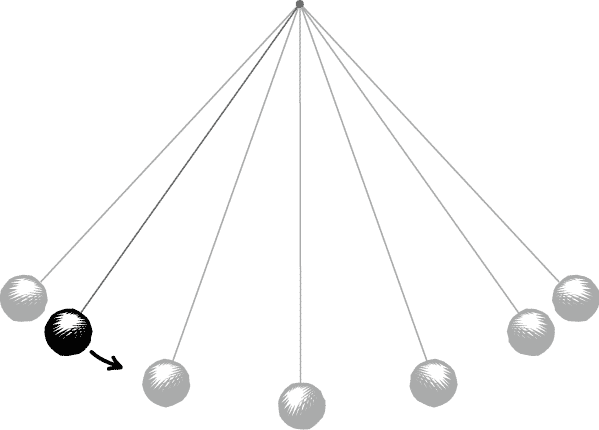
\includegraphics[width=0.8\linewidth]{Pictures/pendulum13}			
				\end{center}
			\end{column}	
			\begin{column}{.50\linewidth}
				\begin{center}
					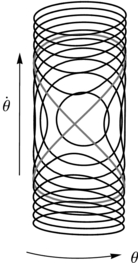
\includegraphics[width=0.45\linewidth]{Pictures/pendulum-phase-space}			
				\end{center}
			\end{column}	
		\end{columns}
		%
		\begin{defblock}[Symplectic Manifold]
			\includestandalone[width=0.95\textwidth]{Pictures/Figure_sym}	
		\end{defblock}
		%
		\begin{exblock}[$M = T^\ast Q$ is symplectic]
			$\omega = d \theta $ with
			$$ \left.\theta\right\vert_{(q,p)} (v) = p (\pi_\ast v) ~.$$
		\end{exblock}
	\end{column}
	\vrule{}
	\pause
	\begin{column}{.50\linewidth}
		\centering
		\textit{ "algebraic approach" to mechanics \dots}
		\vspace{1em}	
		\begin{defblock}[Classical Observables]
			Unital, associative, commutative algebra $C^\infty(M)$.
		\end{defblock}
		%
		\vspace{1em}
		\pause
		\begin{defblock}[Hamiltonian vector fields]
			$v_f \in \mathfrak{X}(M)$ such that:
			$$\iota_{v_f} \omega = -df \quad \text{(exact)}$$ %$\in B^1(M)$
			\small$v_f$ = \emph{Ham.v.f. pertaining to $f\in C^\infty(M)$}.
		\end{defblock}
		%
		\begin{defblock}[Poisson Algebra of Observables]
			$C^\infty(M)$ is a Poisson algebra with
			$$\{f,g\} = \iota_{v_g} \iota_{v_f} \omega = \omega(v_f,v_g) ~.$$
		\end{defblock}
	\end{column}
\end{columns}
\end{frame}
\note[itemize]{
	\footnotesize

	\item We work in the framework of multisymplectic geometry which is one of the possible generalizations of the well-established field of symplectic geometry.
	
	\item To recall what symplectic geometry is let me assume a particular point of view: mechanics.
	\\
	Idea:"
	Symplectic geometry is a branch of differential geometry studying symplectic manifolds; it originated as a formalization of the mathematical apparatus of classical mechanics and geometric optics."{\href{https://ncatlab.org/nlab/show/symplectic+geometry}{nlab}}
	
	Namely, a sym. mfd. is the geometric structure encoding the phase space of conservative, ordinary, classical, mechanical systems.
	
	\item $\theta$ = \emph{tautological 1-form}.
		$\theta$ evaluated at $p\in T^*Q$ in the fibre of $q\in Q$ and contracted with $v$ coincides with the form $p$ evaluated at $q$ and contracted with the push forward of $v$.
	
	\item We identify a special class of vector fields.
		Out of them one can define a Lie bracket.
	
	\item Poisson is a Lie algebra with the extra property of compatibility with the associative product (Leibniz rule)
}
%-------------------------------------------------------------------------------------------------------------------------------------------------

%------------------------------------------------------------------------------------------------
% Frame inspired by Leonid: passing from moment maps to comoment maps
\begin{frame}[fragile]{Reminder: Moment maps in symplectic geometry}
	Let $(M,\omega)$ be a symplectic manifold, $\vartheta: G\times M \to M$ a Lie group action preserving $\omega$ and $v:\mathfrak{g}\to \mathfrak{X}(M)$ the corresponding infinitesimal action
	%
		\begin{defblock}[Moment map pertaining to $\vartheta$]
			Smooth map $ \mu: M \to \mathfrak{g}^\ast$ such that: \stackunder{$d \langle\mu , \xi \rangle = \iota_{v_\xi}\omega \scriptstyle\quad \forall \xi \in \mathfrak{g}$}{$f (\vartheta_g(x)) = Ad^\ast_g (f(x)) \scriptstyle\quad \forall g \in G, x \in M$}
		\end{defblock}
	%
	\vfill
	\emph{... from a dual perspective (assuming $G$ connected) ...}
			\begin{defblock}[Comoment map pertaining to $v$]
				\begin{columns}
					\begin{column}{.5\linewidth}	
			Lie algebra morphism \qquad $ f: \mathfrak{g} \to C^\infty(M) $
			\\
			such that \qquad $ d~f (x) = -\iota_{v_x} \omega \qquad \forall x \in \mathfrak{g}~.$
					\end{column}
					\begin{column}{.4\linewidth}	
						\begin{displaymath}
							\begin{tikzcd}
								& C^{\infty}(M,\omega) \ar[d]
								\\
								\mathfrak{g} \ar[ur,dashed,"(f)"]\ar[r,"v"']& \mathfrak{X}(M)
							\end{tikzcd}	
						\end{displaymath}
					\end{column}
				\end{columns}
		\end{defblock}		
	%
	\emph{... a tool encoding conserved quantities ...}
	\begin{propblock}[Noether Theorem]
		\small Fixed $H\in C^\infty_{\text{Ham}}(M)$ ($\mathfrak{g}$-invariant) ,
				\qquad
				$\mathcal{L}_{v_H} f(x) = 0 \qquad \forall x \in \mathfrak{g}~.$
	\end{propblock}
\end{frame}
\note[itemize]{
	\item comoment map is a Lie algebra morphism projecting to $v$. (Triangle diagram in Lie algebra category).
}



%------------------------------------------------------------------------------------------------
\begin{frame}{Geometry of symmetries}\label{frame:geometrysymmetries}
	Basic mechanical structures are encoded in geometry. but there is another complementary geometrical property that's natural in physics: symmetry!
	\begin{alertblock}{Upshot}
		Continous symmetries are described by actions of a Lie group on $M$.
	\end{alertblock}
	\begin{block}{Noether}
		Presence of symmetries $\quad \Rightarrow \quad$ existence of conserved quantities.
	\end{block}	
	\begin{block}{Key concept:}
		Noether current are encoded in a \emph{moment map}  $\mu :M \rightarrow \mathfrak{g}^*$ (the dual of the comoment map $f$. 
	\end{block}
  \begin{columns}[T]
   	\begin{column}{.6\textwidth}
			\begin{block}{Symplectic reduction:}
			\begin{itemize}
				\item System dynamics should be restricted to level set of conserved observables in order to efficiently store dynamical properties.
				\item Under certain assumptions, $\mu^{-1}( 0 )/G$ is a symplectic manifold with an "induced" symplectic structure.
			\end{itemize}
			\end{block}
    \end{column}
    \begin{column}{.4\textwidth}	
			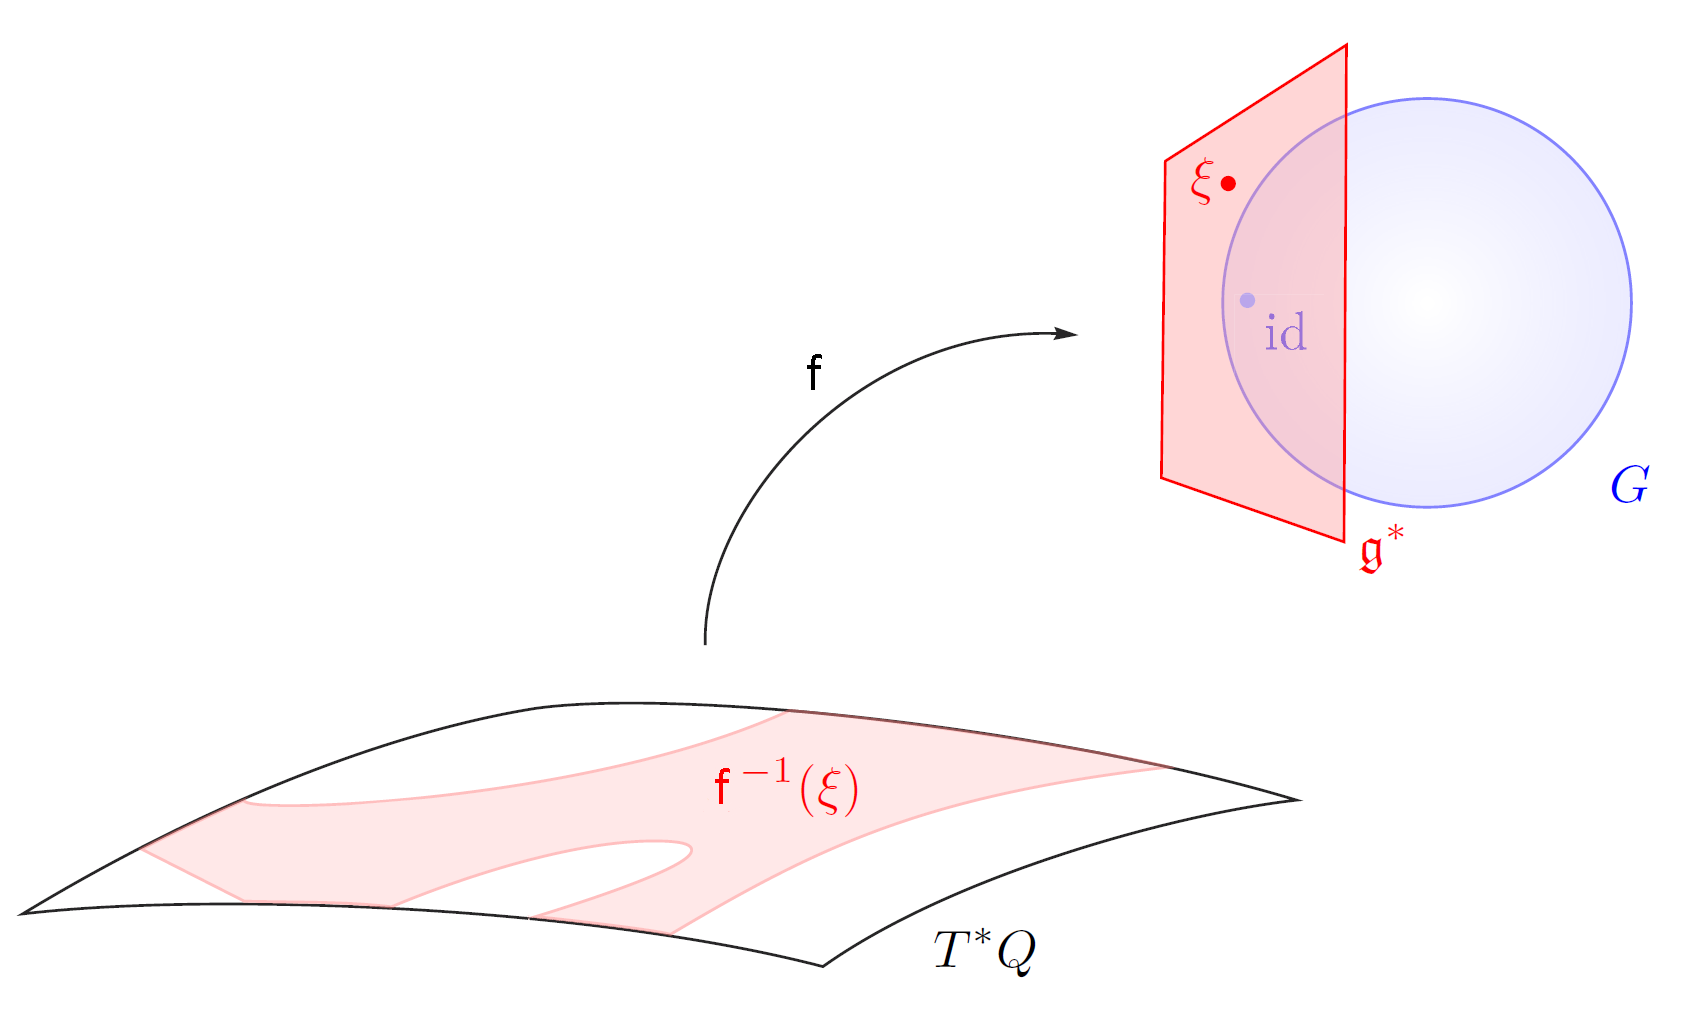
\includegraphics[width=\textwidth]{Pictures/Reduction} 
  	\end{column}
	\end{columns}			
\end{frame}
\note[itemize]{
	\item
}
%------------------------------------------------------------------------------------------------




%-------------------------------------------------------------------------------------------------------------------------------------------------
\subsection{MultiSymplectic Manifolds}
%-------------------------------------------------------------------------------------------------------------------------------------------------


%------------------------------------------------------------------------------------------------
\begin{frame}[fragile]{MS geometry and classical field mechanics}
		Consider a smooth manifold $Y$,
		\begin{columns}
			\hfill
			\begin{column}{.5\linewidth}
				\emph{Multicotangent bundle} $\bigwedge = \bigwedge^n T^\ast Y$\\
				is naturally $n$-plectic
			\end{column}
			\begin{column}{.4\linewidth}
				\[
				\begin{tikzcd}
					\Lambda \ar[d,"\pi"'] & T \Lambda \ar[d,"T \pi"] \ar[l] \\
					Y								& T Y \ar[l]
				\end{tikzcd}	
				\]
			\end{column}
		\end{columns}
	\pause
	\begin{defblock}[Tautological $n$-form]
		$\theta \in \Omega^n(\Lambda)$ such that:
		\begin{displaymath}
		\begin{split}
			\left[ \iota_{u_1 \wedge \ldots \wedge u_n} \theta \right]_\eta 
			&= \iota_{(T \pi)_\ast u_1 \wedge \ldots \wedge (T \pi)_\ast u_n} \eta \\
			&= \iota_{u_1 \wedge \ldots \wedge u_n} \pi^\ast \eta 
			\qquad \qquad \forall \eta \in \Lambda \, , \: \forall u_i \in T_\eta \Lambda 		
		\end{split}
		\end{displaymath}
	\end{defblock}
	\vfill
	\begin{columns}
		\begin{column}{.6\linewidth}
			\begin{defblock}[Tautological (multisymplectic) (n+1)-form]
				$$\omega := d \theta$$
			\end{defblock}
		\end{column}
		\begin{column}{.4\linewidth}
		 	\begin{claimblock}$\omega$ is not degenerate.\end{claimblock}	
		\end{column}
	\end{columns}	
	\pause
	\begin{keywordblock}
		\begin{tabular}{|c|c|c|}
			\hline 
			point-particles mechanics & $\rightsquigarrow$ & classical fields mechanics \\
			%(finite discrete DOF) & & (finite dimensional continuous DOF) \\
			\hline 
			symplectic & $\rightsquigarrow$ & multisymplectic \\ 
			\hline 
			Observables (Poisson) algebra & $\rightsquigarrow$ & Observables $L-\infty$ algebra
			 \\ 
			\hline 
			Co-moment map & $\rightsquigarrow$ & Homotopy co-momentum map \\ 
			\hline 
		\end{tabular} 
	\end{keywordblock}

	
\end{frame}
\note[itemize]{
	\item This example is significant from the perspective of geometric classical field theory:
		\begin{displaymath}
			\frac{\text{classical mechanics}}{\text{symplectic geo.}} =
			\frac{\text{classical field mechanics}}{\text{multisymplectic geo.}}
		\end{displaymath}
	\item Multicotangent bundle is the \emph{Higher analogue} of the cotangent bundle.
	(but it is not yet the analogue of a \emph{phase space}.)
\item The multiphase space is the sub-bundle of $n$-forms vanishing when contracted with 2 vertical fields.
  	\item The reason why this sub-bundle has a particular role is that it can be proved to be isomorphic to a suitable dual of the first Jet bundle.
  	\item For further details see Gotay et al. \href{https://arxiv.org/abs/physics/9801019}{arXiv:physics/9801019}. For a pictorial representation of all the structures involved in the geometric mechanics of I order classical field theories see appendix, pag: \ref{frame:Gimmsy}.
}
%------------------------------------------------------------------------------------------------

%------------------------------------------------------------------------------------------------
  \begin{frame}[fragile]{GIMMSY construction} \label{frame:Gimmsy}
  		\includestandalone[width=0.90\textwidth]{Pictures/Figure_ms_landscape}  	
  \end{frame}
  \note{}
%------------------------------------------------------------------------------------------------

	
	
	
%------------------------------------------------------------------------------------------------
\begin{frame}{Special classes of smooth objects} 
  	\begin{columns}
		\begin{column}[t]{.42\linewidth}		
			\begin{defblock}[Hamiltonian v.f.]
				$\mathfrak{X}_{ham} =  \left\lbrace X \in  \mathfrak{X} \right\vert \left. \iota_x \omega \textrm{ exact}  \right\rbrace$ 			
			\end{defblock}
			\begin{defblock}[Multisymplectic v.f.]
				$\mathfrak{X}_{ms} =  \left\lbrace X \in  \mathfrak{X} \right\vert \left. \mathcal{L}_X \omega = 0  \right\rbrace$ 	
			\end{defblock}
		\end{column}
		\begin{column}[t]{.58\linewidth}		
			\begin{defblock}[Hamiltonian $(n$-$1)-$forms]
				\begin{displaymath}
					\Omega^{n-1}_{ham} 	:=
					\biggr\{ H \in  \Omega^{n-1} \; \left\vert \; 
					\stackanchor{$\exists X \in \mathfrak{X}_{ham}$}{: $d H = -\iota_X \omega$} \right\} 
			\end{displaymath}
			\end{defblock}		
		\end{column}
  	\end{columns}
  	%
  	\vspace{0.5em}
  	%
  	\onslide<2->{
  	\begin{columns}
		\begin{column}[t]{.5\linewidth}	
			\centering\emph{Global symmetries}
			\begin{defblock}[Multisymplectic (Lie group) action]
				$\Phi: G \circlearrowright (M, \omega)$ \emph{right action} s.t. \\
				$$\hat{\Phi}(g)_\ast \omega = \omega \quad \forall g \in G$$
			\end{defblock}
		\end{column}
		\begin{column}[t]{.5\linewidth}			
			\centering\emph{Infinitesimal symmetries}
			\begin{defblock}[Multisymplectic (Lie algebra) action]
				$V: \mathfrak{g} \rightarrow \mathfrak{X} (M)$ \emph{Lie algebra morphism} s.t. \\
				$$\mathcal{L}_{V_\xi} \omega = 0 \quad \forall \xi \in \mathfrak{g}$$	
			\end{defblock}
		\end{column}
  	\end{columns}
  	}
  	%
  	\onslide<3->{		
	  	\begin{asideblock}[Hierarchy of conserved quantities]%Shades of...
	  		\begin{table}[] % http://tablesgenerator.com/
			\begin{tabular}{lllll}
					& strictly conserved & & & $\mathcal{L}_X \alpha= 0$ \\
				$\alpha \in \Omega^\bullet$ & globally conserved & along $X \in \mathfrak{X}$ & $\Leftrightarrow$ & $\mathcal{L}_X \alpha\in B $ (exact) \\
				  & locally conserved  & & & $\mathcal{L}_X \alpha\in Z $ (closed)                                
			\end{tabular}
			\end{table}
	  	\end{asideblock}
  	}
  	
  \end{frame}
  \note[itemize]{
  	\item Exactly as it happens in symplectic geometry, fixing a smooth form $\omega$ on $M$ yields a criterion for classifying vector fields and differential forms.
  	\\(Pay attention to the sign convention in defining the Hamiltonian vector fields)
  	\item Also, we can naturally select a special class of symmetries (global and infinitesimal) which preserve the fixed multisymplectic form.
  	\item Aside, we can start to see that, in this setting, measurable quantities are not only smooth functions but also differential forms with degree greater then zero.
  	For such objects can be defined weaker notions of conservation along a flow.
  	\item The idea to consider forms of various degree as observables do not fall out of the sky. 
  		For instance in a string there will be two kind of measurable quantities: extensive observable (1-forms), like the density, and intensive observables (0-forms), like the tension. 
 		%\href{https://en.wikipedia.org/wiki/Intensive_and_extensive_properties#Intensive_properties}{(wiki link on this terminology)}
  	\item Starting from this observation we can define the space of all possible observables (see next slide).
  }
%---------------------------------------------------------------------------------------------------------------------------------------------------


%-------------------------------------------------------------------------------------------------------------------------------------------------
\subsection{$L_\infty$-algebras}
%-------------------------------------------------------------------------------------------------------------------------------------------------

%---------------------------------------------------------------------------------------------------------------------------------------------------
\begin{frame}[fragile,shrink]{Unwrapping the \emph{higher Jacobi equations}}\label{Frame:unwapping-Jacobi}
\underline{Slogan:} \emph{Jacobi identity satisfied up to an higher coherent homotopy}
		%
		\vspace{1.5em}
		\begin{columns}[c]
			\hfill
			\begin{column}{0.5\linewidth}
				Higher Jacobi implies:
				\begin{itemize}  \setlength\itemsep{1em}
					\item Underlying chain-complex $(L,\mu_1)$ with differential $d=\mu_1$;
					\item \color{red} $\mu_2 = [\cdot,\cdot]$ is a chain map $L^{\otimes 2} \to L$;
					\item \color{green!20!black}$\mu_3=j(\cdot,\cdot,\cdot)$ is a chain homotopy 
						$\mu_2\circ\mu_2 \Rightarrow 0$;
						\\ i.e. between the usual Jacobiator ${[[\cdot,\cdot],\cdot]} \circ P_{\text{unsh}}$ and the $0$ map 
					\item \color{purple}higher analogues...	
					\\ e.g. $\mu_4$, is a second order chain-homotopy between the two chain homotopies  ${[j(\cdot,\cdot ,\cdot]),\cdot]}\circ P_{\text{unsh}}$ and ${j([\cdot , \cdot],\cdot,\cdot)}\circ P_{\text{unsh}}$
				\end{itemize}
			\end{column}
			\begin{column}{0.45\linewidth}
				\includestandalone[width=0.9\linewidth]{Pictures/Figure_Linfinity_diagram}
			\end{column}	
		\end{columns}	
		\vspace{1.5em}
		Notation: $P_{\text{unsh}}$ = sum on all the possibile unshuffled permutation.

\end{frame}
\note[itemize]{
  \item Regarding any $l_k$ as a tree with $k$ entries and 1 output, the $k$-th generalized Jacobi equation is produced summing all the possible way to obtain a $k+1$-ary tree by composing two other trees (not more then two!).
  \item Can be regarded as
  	\begin{displaymath}
  		\sum_{i+j = k} l_j \circ ( l_j \otimes \mathbb{I}) \circ P_{\text{unsh}}
  	\end{displaymath}
  	Where $P_{\text{unsh}} : L^{\otimes(k-1)} \rightarrow L^{\otimes(k-1)} $ is the $(i,j)$-unshuffolator.
  	\\(you consider only unshuffles to avoid the redundancies given by the fact that any $l_i$ has fixed symmetry.
  \item Examples of unshuffles: \\
  \begin{displaymath}
  \begin{split}
  	(12)(3)\quad(13)(2)\quad(23)(1)\\
  	(123)(4)\quad(234)(1)\quad(134)(2)\quad(124)(3)\\
  	(12)(34)\quad(23)(14)\quad(13)(24)\quad(14)(23)\quad(24)(13)
  \end{split}
  \end{displaymath}
	\item When regarding the L$\infty$ structure as a chain complex with homotopies you get a neat intepretation of the Jacobi identity at the price that \emph{graded skew-symmetry} definition is more obscure than in the presentation with graded vector spaces.
}
%------------------------------------------------------------------------------------------------



%-------------------------------------------------------------------------------------------------------------------------------------------------
\subsection{Observables $L_\infty$-algebra}
%-------------------------------------------------------------------------------------------------------------------------------------------------

%------------------------------------------------------------------------------------------------
\begin{frame}{Lie $\infty$-algebra of Observables \emph{(Rogers)}}
	\begin{defblock}[$L_\infty$-algebra \emph{(Lada, Stasheff) \cite{Lada1993}}]
		\includestandalone{Pictures/Figure_Linfinitydef}
	\end{defblock}	
	%
	\pause
	\vfill
	\begin{thmblock}[Rogers \cite{Rogers2010}]
		The \emph{higher observable algebra} $L_{\infty}(M,\omega)$ 	forms an honest $L_\infty$ algebra.
		\footnotetext{Take $[\cdot]_1$ equal to the deRham differential.}
	\end{thmblock}
\end{frame}
\note[itemize]{
	\item $L_\infty$-algebra is the notion obtained from a Lie algebra requiring that the Jacobi identity is satisfied only up to a higher coherent chain homotopy.
	\item The Lie-n algebra mentioned before is a $L_\infty$ algebra with underlying graded vector space concentrated in degrees $0,1...n$.
	
	\item Definition. We say that a permutation $\sigma \in S_n$ is a $(j,n-j)$-unshuffle, $0\leq j \le1 n$  if $\sigma(1)< \dots < \sigma(j)$ and $\sigma(j+1)<\dots<\sigma(n)$.
	\\
	You can also say that $\sigma$ is a $(j,n-j)$-unshuffle if $\sigma(i)< \sigma(i+1)$ when $i\neq j$.

	\item 	Alternatively, the Jacobiators can be also denoted as $$\displaystyle J_m=\sum_{i+j=m+1}(-)^{i(j+1)} 	\mu_i \circ \mu_j = 0$$
	employing the so-called \emph{ Richardson-Nijenhuis product}
		 $\mu_i\circ \mu_j := \frac{1}{j!(i-1)!}\mu_i\cdot\mu_j \cdot \mathcal{A}~, \qquad \mathcal{A} =$ (graded) total skew-symmetrizator.
		 
	\item see frame extra-\ref{Frame:unwapping-Jacobi} for a slightly demystification of the higher Jacobi equations.

	\item more precisely this statement is a proposition/definition

}
%------------------------------------------------------------------------------------------------


%------------------------------------------------------------------------------------------------
%Slide by Leonid
\begin{frame}[fragile]{Why the $L_\infty$ algebra of observable is so "simple"}
	\textit{(in the sense that the higher brackets are defined only on $L^0$, i.e. "grounded")}
	 \\
	 \vfill
	Extend the underlying cochain complex
	\begin{displaymath}
		\begin{tikzcd}
			C^{\infty}(M) \ar[r,"d"] &
			\cdots \ar[r,"d"] &
			\Omega^{n-2}(M) \ar[r,"d"] &
			\Omega^{n-1}_{Ham}(M,\omega) \ar[r,dashed] &
			\mathfrak{X}_{Ham}(M,\omega)
		\end{tikzcd}
	\end{displaymath}
	Consider 
	\begin{displaymath}
		\begin{tikzcd}[column sep= small,row sep=0ex]
			\{\cdot,\cdot\}_2 ~\colon&[-1em] \left(\Omega^{n-1}_{\textrm{Ham}}(M,\omega)\right)^{\otimes 2} 	\arrow[r]& 				\Omega^{n-1}(M) \\[-1ex]
			& \sigma_1\otimes\sigma_1 	\ar[r, mapsto]& 	-
			\iota_{\mathscr{v}_{\sigma_1}}\iota_{\mathscr{v}_{\sigma_2}}\omega 
		\end{tikzcd}
	\end{displaymath}
	%
	\vfill
	\begin{thmblock}[Barnich, Fulp, Lada, Stasheff \cite{Barnich1998}]
		 Let $L^\bullet = (\cdots \rightarrow L^{-1} \rightarrow L^0 \rightarrow \mathfrak{g})$ be a resolution of the Lie
		algebra $\mathfrak{g}$.
		\begin{itemize}
			\item a skew symmetric $\ell_2:L^0\times L^0 \to L^0$ covering the Lie bracket of $\mathfrak{g}$ can extended to a $L_\infty$-algebra structure $\{\ell_k\}$ on $L_\bullet$.
			\item If $\ell_2$ is zero on boundaries, then the structure can be chosen such that $\ell_i$, for $i\geq 2$, are non-zero only on $L^0$.
		\end{itemize}
	\end{thmblock}


\end{frame}
\note[itemize]{
	\item resolution in the sense that the $0$-th homology group is isomorphic to $\mathfrak{g}$ and all other cohomology groups are trivial (\cite[\S 2.1]{Barnich1998})
	\item the extended complex is a resolution only if $M$ is contractible. In other terms, such a resolution exists locally on any multisymplectic smooth manifold.

}



%------------------------------------------------------------------------------------------------


%-------------------------------------------------------------------------------------------------------------------------------------------------
\subsection{Homotopy comoment maps}
%-------------------------------------------------------------------------------------------------------------------------------------------------


\begin{frame}{Comoment maps}
	Consider a Lie algebra action $v:\mathfrak{g} \to \mathfrak{X}(M)$  preserving the $n$-plectic form $\omega$,
	\vfill
	\begin{columns}
		\begin{column}{.5\linewidth}	
	\textbf{Symplectic case $(n=1)$}
		\begin{defblock}[Comoment map pertaining to $v$]
			Lie algebra morphism
			$$ f: \mathfrak{g} \to C^\infty(M) $$
			such that
			$$ d~f (x) = -\iota_{v_x} \omega \qquad \forall x \in \mathfrak{g}~.$$
		\end{defblock}		
		\end{column}
		\begin{column}{.5\linewidth}	
	\textbf{Multi-symplectic case $(n\geq 1)$}
		\begin{defblock}[Homotopy comoment map \tiny (HCMM)]
			$L_\infty$-morphism 
			$$ (f_k) : \mathfrak{g} \to L_\infty (M,\omega)$$
			such that
			$$ d~f_1(x) = -\iota_{v_x} \omega \qquad \forall x \in \mathfrak{g}~.$$
		\end{defblock}		
		\end{column}
	\end{columns}	
	%
	\pause
	\centering \textbf{-- Conserved quantities --}
	%
	\begin{columns}
		\begin{column}{.5\linewidth}		
			\begin{propblock}[Noether Theorem]
				\small Fixed $H\in C^\infty_{\text{Ham}}(M)$ ($\mathfrak{g}$-invariant) ,
				$$\mathcal{L}_{v_H} f(x) = 0 \qquad \forall x \in \mathfrak{g}$$
			\end{propblock}
		\end{column}
		\begin{column}{.5\linewidth}			
			\begin{propblock}[RWZ16 Theorem]
				\small Fixed $H\in \Omega^{n-1}_{\text{Ham}}(M)$ ($\mathfrak{g}$-invariant),
				$$\mathcal{L}_{v_H} f_k(p) \in B^k(M) \qquad \forall p \in Z_k(\mathfrak{g})$$			
			\end{propblock}
		\end{column}
	\end{columns}



\end{frame}
\note[itemize]{
	\item  An infinitesimal symmetry is a lie algebra morphism such that $\mathcal{L}_{v_x} \omega = 0 ~ \forall x \in \mathfrak{g}$.
	\\ (It is also call an infinitesimal multisymplectic action and $v_x$ is the infinitesimal generator of the action, corresponding to $x \in \mathfrak g$.) 
	\item Essentially, admitting a comoment maps mean that $v$ acts via Hamiltonian vector fields.
	\item In mechanical terms, a moment map is a tool associated with a Hamiltonian action of a Lie group on a symplectic manifold, used to construct conserved quantities for the action.
	\item The name derives from the special case given by angular momentum in the dynamics of rigid bodies, 
	\item Notation [RWZ16]: H is called \emph{strictly invariant} and $f_k(p)$ are \emph{globally invariant}.
	\\
	$B^k(M)$ are exact differential k-forms and $Z_k(\mathfrak{g}$ are Eilenberg Chevalley homology k-cycles.
	
	\item Details about Reduction in frame \ref{frame:geometrysymmetries} of the  appendix.
	
}
%-------------------------------------------------------------------------------------------------------------------------------------------------

%------------------------------------------------------------------------------------------------
  \begin{frame}[fragile,t]{Chevalley-Eilenberg Complex \hfill\hyperlink{frame:hcmm-main}{\beamerreturnbutton{}}}\label{frame:CE-complex}
  	Consider $\mathfrak{g}$, Lie Algebra.
  	\begin{defblock}[Eilenberg-Chevalley Complex]
  		Chain Complex
			\begin{center}
				\begin{tikzcd}[column sep= small,row sep=0.25ex]
					\ldots \ar[r,"\partial"] & \wedge^k \mathfrak{g} \ar[r,"\partial"] & 
					\wedge^{k-1} \mathfrak{g} \ar[r,"\partial"] & \ldots
			\end{tikzcd}	
			\end{center}
			with chain group
			\begin{displaymath}
				C^k := \wedge^k \mathfrak{g} \equiv 
				\big\{ c : \mathfrak{g}^\ast\times\ldots\mathfrak{g}^\ast \to \mathbb{R}\:\big\vert\, \textrm{alternating, k-linear} \big\}
			\end{displaymath}
			and boundary operator defined as
			$\partial \equiv \partial^k :  \Lambda^{k} {\mathfrak g} \to \Lambda^{k-1} {\mathfrak g}$  via
			$$
				\partial (\xi_1 \wedge \xi_2 \wedge \dots \wedge \xi_k) := \sum_{1\leq i< j \leq k} (-1)^{i+j}\, [\xi_i, \xi_j] \wedge \xi_1 \wedge \dots {\hat \xi}_i \wedge \dots \wedge {\hat \xi}_j \wedge \dots \xi_k
			$$
			where $\hat{}$ denoting deletion and with $\partial_0 = 0$.
  	\end{defblock}
		\begin{claimblock}
			$$\partial^2 = 0$$
		\end{claimblock}		
  \end{frame}
\note[itemize]{
	\item
}
%----------------------------------------------------------------------------------------------


%-------------------------------------------------------------------------------------------------------------------------------------------------
\begin{frame}[fragile]{Homotopy co-moment maps \emph{(Callies, Fregier, Rogers, Zambon)}}
	Consider a multisymplectic action $G \circlearrowright (M, \omega)$,
	\pause
	\begin{lemblock}[HCMM unfolded  \cite{Callies2016}]
			%
			HCMM is a sequence of (graded-skew) multilinear maps:
			\begin{displaymath}
				(f)  = \big\lbrace f_k: \; \Lambda^k{\mathfrak g} \to L^{1-k} \subseteq \Omega^{n-k} 
				\;\big\vert\; 0\leq k \leq n+1  \big\rbrace
			\end{displaymath}
			%
			\vspace{-.5em}	
			\includestandalone[width=0.9\textwidth]{Pictures/Frame_HCMM}
			
			\vspace{-1em}		
			\emph{fulfilling:}%\emph{such that:}
			\begin{itemize}
				\item<2-> $f_0 = 0 $, $f_{n+1} = 0$
				\item<3-> $d f_k (p) = f_{k-1} (\partial p)  - (-1)^{\frac{k(k+1)}{2}} \iota(v_p) \omega 
				\qquad\scriptstyle \forall p \in \Lambda^k(\mathfrak{g}),\; \forall k=1,\dots n+1$
			\end{itemize}
		\end{lemblock}



\end{frame}
\note[itemize]{
	%\item 		Consider:  $v:\mathfrak g\to \mathfrak X(M)$  a Lie algebra morphism  s.t. $\mathcal{L}_{v_x}\omega=0 \quad  \forall x\in\mathfrak g$ (i.e infinitesimal multisymplectic Lie algebra action $\mathfrak{g}\circlearrowleft (M,\omega)$)
	\item More conceptually, a comoment is an $L_\infty$-morphism $(f):\mathfrak{g}\to L_\infty(M,\omega)$ lifting the action $v:\mathfrak{g}\to \mathfrak{X}(M)$, 
i.e. making the diagram commute in the $L_\infty$-algebras category.
	\item The vertical arrow is the trivial $L_\infty$-extension of the function mapping any Hamiltonian form to the unique corresponding Hamiltonian vector field (an it is zero elsewhere)
		\\
		(Note that any Lie algebra can be seen as an $L_\infty$-algebra concentrated in degree $0$, therefore any $L_\infty$-morphism $L\to\mathfrak{g}$ is simply given by a linear map $L_0 \to \mathfrak{g}$ preserving the binary brackets.)
	\item We will make use of an explicit version of this definition which is expressed by the lemma.
	 Practically speaking, a HCMM is given by several multilinear maps ...
	 \item In the equation we have tacitly set $\Lambda^{-1}(M) = 0$
	 %\item Notation: \qquad $\partial =$ Chevalley-Eilenberg boundary operator.
	%\item Notice that a HCMM pertains to an "infinitesimal" action of ${\mathfrak g}$ on $M$ with ${\mathfrak g}$ being the Lie algebra of a generic Lie group $G$, acting on $M$ by $\omega$-preserving vector fields.
		\item (Notation) $ p = \xi_1 \wedge \xi_2 \wedge \dots \wedge \xi_k$, 
			then $v_p = v_1 \wedge v_2 \wedge \dots \wedge v_k$ 
			where $v_i \equiv v_{\xi_i}$ are the fundamental vector fields associated to the action $G \circlearrowright M$.
	%	\item (Notation) $\iota(v_p) \omega = \iota(v_k)\dots\iota(v_1) \omega$
	%	\item $\varsigma(k) := - (-1)^{\frac{k(k+1)}{2}}$ 
		\item (Notation) $(\iota^{k}_{\mathfrak{g}}\omega)(p):= \iota(v_p) \omega = \iota(v_k)\dots\iota(v_1) \omega$
		\item $\partial \equiv \partial_k:  \Lambda^{k} {\mathfrak g} \to \Lambda^{k-1} {\mathfrak g}$  is the usual Eilenberg-Chevalley complex boundary operator (see appendix, pag: \ref{frame:CE-complex});
%		\item The definition tells us that the {\it closed} forms
%			$$\mu_k := f_{k-1} (\partial p) +  \varsigma(k) \iota(v_p) \omega 	$$
%			must actually be {\it exact}, with potential $-f_k(p)$.  	
		\item The last equation tells us that an HCMM is not a chain complex morphism but is rather a chain complex homotopy between 0 and the multicontraction $\alpha=(\iota^{k}_{\mathfrak{g}}\omega)$ (see next slide).
		is a chain map by lemma 2.18 \cite{Ryvkin2016}).
}
%---------------------------------------------------------------------------------------------------------------------------------















%===================================================================================
\section{Foreground}
%===================================================================================

%-------------------------------------------------------------------------------------------------------------------------------------------------
\subsection{Work Done with Leonid}
%-------------------------------------------------------------------------------------------------------------------------------------------------
%\subsectiontitle


%-------------------------------------------------------------------------------------------------------------------------------------------------
\begin{frame}[fragile]{Cohomological obstruction to HCMM \hfill\hyperlink{frame:introcohoobstruction}{\beamerreturnbutton{}}}\label{frame:AppCohomoObstructions}
	Let $(M,\omega)$ multisymplectic and $\vartheta: M \times G \to M$ preserves $\omega$. 
	\vfill
	A HCMM is a sequence of linear maps:
	\vspace{-.5em}
	\begin{displaymath}
		(f)  = \big\lbrace f_k: \; \Lambda^k{\mathfrak g} \to L_{k-1} \subseteq \Omega^{n-k} 
		\;\big\vert\; 0\leq k \leq n+1  \big\rbrace
	\end{displaymath}	
	\vfill		
	\emph{It can be interpreted as primitives of a certain cocycle in the total complex of}
	\vspace{-.5em}
	\begin{displaymath}
		\Big(C_\mathfrak{g}^{\bullet,\bullet} = \Lambda^{\geq 1} 
		\mathfrak{g}^*\otimes \Omega^\bullet(M) 
		\cong Hom(\Lambda^\bullet \mathfrak{g},\Omega^\bullet),~\delta_\text{CE},~d\Big)
		~,	
	\end{displaymath}
	\vfill
	%
	\pause
	\begin{propblock}[$\vartheta ~\text{admits HCMM}~ ~\Longleftrightarrow~ \lbrack\tilde{\omega}\rbrack=0\in H^{n+1}(C_\mathfrak g^\bullet,d_ {tot})$	
	]
		Where:
		\begin{columns}
		\begin{column}{.5\textwidth}
			\begin{displaymath}
				\tilde{\omega} = \sum_{k=1}^{n+1} (-1)^{k-1} \iota^k_\mathfrak{g} \omega \in C_\mathfrak{g}^{n+1},
			\end{displaymath}		
		\end{column}
		\begin{column}{.5\textwidth}
			\begin{align*}
				\iota^k_\mathfrak{g} \colon \Omega^\bullet(M)
				&\to \Lambda^k \mathfrak{g}^\ast \otimes \Omega^{\bullet-k}(M)
				\\ \omega&\mapsto \omega_k = 
				\left(p \mapsto \iota_{v_p} \omega  \right) ,
			\end{align*}
		\end{column}		
		\end{columns} 
	\end{propblock}
	%
\end{frame}
\note[itemize]{
	\item 
	The  corresponding total complex is given by
	\begin{displaymath}
		(C_\mathfrak{g}^{\bullet}, d_\text{tot} = 
		\delta_\text{CE}\otimes \text{id} + \text{id}\otimes d),
	\end{displaymath}
	where $d$ denotes the de Rham differential and $\delta_{CE}:\Lambda^k\mathfrak g^*\to \Lambda^{k+1}\mathfrak g^*$ the Lie algebra cohomology differential.
	According to the Koszul sign convention, $d_{\text{tot}}$ acts on an element of $\Lambda^k \mathfrak{g}^*\otimes \Omega^\bullet(M)$ as $\delta_\text{CE} + (-1)^k d$.
	
	\item the multicontraction $\alpha=(\iota^{k}_{\mathfrak{g}}\omega)$ 	is a chain map by lemma 2.18 \cite{Ryvkin2016}).

	\item PROP: the primitives of the natural cocycle $\tilde{\omega}$ are in one-to-one correspondence with comoments of $v$.
	

}
%-------------------------------------------------------------------------------------------------------------------------------------------------




%-------------------------------------------------------------------------------------------------------------------------------------------------
\begin{frame}[fragile]{Cohomological obstructions for compact groups \hfill\hyperlink{frame:obstructioncompactgroups}{\beamerreturnbutton{}}}\label{frame:cohomologicalproposition}
	Let $\vartheta:G\times M\to M$ be a compact Lie group acting on a pre-multisymplectic manifold, preserving the pre-multisymplectic form $\omega$. 
	%
	\begin{propblock}
		[ $\exists$ (HCMM) $ 
			~\Leftrightarrow~ 
			\lbrack\vartheta^*\omega-\pi^*\omega\rbrack=0\in H^{n+1}(G\times M)$]
		Based on the sequence of isomorphisms:
		\begin{center}
			\begin{tikzcd}
	 			\Omega^\bullet(M,\vartheta) \ar[d,"\vartheta^\ast-\pi^\ast"] &\quad
				 & H_\text{dR}(M) \ar[d,"\vartheta^\ast-\pi^\ast"]  
				 & \lbrack \omega \rbrack \ar[d,mapsto]
				 \\ 
				 \Omega^\bullet(G\times M, r\times id) \ar["\cong",leftrightarrow]{d} &\quad
				 & H_\text{dR}(G\times M) \ar[leftrightarrow,"\cong"]{d}[swap]{\text{\tiny (K\"unneth)}} 
				 & \lbrack \vartheta^\ast \omega - \pi^\ast \omega \rbrack \ar[ddd,mapsto]
				 \\ 
				 \Omega^\bullet(G,r) \otimes \Omega^\bullet(M) \ar["\cong",leftrightarrow]{d}[swap]{} &\quad
				 & H_\text{dR}(G) \otimes  H_\text{dR}(M) \ar[d,"\cong",leftrightarrow]
				 \\ 
				 \Lambda^\bullet \mathfrak{g}^* \otimes \Omega^\bullet(M)\ar["\cong",leftrightarrow]{d} &\quad
				 & H_\text{CE}(\mathfrak{g}) \otimes  H_\text{dR}(M) 
				 \ar["\cong",leftrightarrow]{d} & 
				 \\
				 C_\mathfrak{g}^\bullet \oplus ( \mathbb{R}\otimes \Omega^\bullet(M))&\quad 
				 & H(C_\mathfrak{g}^\bullet)\oplus H_\text{dR}(M)
				 & \lbrack \tilde{\omega}\rbrack
			\end{tikzcd}
		\end{center}						
	\end{propblock}
\end{frame}
\note[itemize]{
	\item
}
%-------------------------------------------------------------------------------------------------------------------------------------------------



%-------------------------------------------------------------------------------------------------------------------------------------------------
\begin{frame}[fragile]{Hints to the relation with equivariant cohomology \hfill\hyperlink{frame:obstructioncompactgroups}{\beamerreturnbutton{}}}\label{frame:EquivariantCohomology}
	\begin{itemize}
	\item 	Let a compact Lie group $G$ act on a manifold $M$. Let $EG$ be a contractible space on which $G$ acts freely by $\vartheta^{EG}$. Then we define the equivariant cohomology of $M$ as $H^\bullet_G(M):=H^\bullet((M\times EG)/G)$, where $G$ acts on $M\times EG$ diagonally.

	\item As $EG$ might not be a manifold, we have to interpret $H^\bullet(\cdot)$ as a suituable cohomology theory (e.g. singular cohomology with real coefficients) in the above definition.
	
	\item As $G$ is compact, when $\vartheta:G\times M\to M$ is a free action, we have $H_G^\bullet(M)=H^\bullet_{dR}(M/G)$. For a not necessarily free action $\vartheta$, we still have the following diagram
	$$
		G\times (M\times EG) \xrightarrow{\vartheta\times \vartheta^{EG}}
		M\times EG \xrightarrow{q} (M\times EG)/G
	$$
	where $q$ is the projection to the orbits, which induces $q^*$ in cohomology.	
	\end{itemize}
		\vfill
	%
	Let $G\times M\to M$ be a compact Lie group preserving a pre-multisymplectic form $\omega$.
	%
	\begin{tcolorbox}
	\begin{itemize}
		\item[\CheckedBox]  Proved, without resorting on a specific model, that if $[\omega]\in H^\bullet(M)$ lies in the image of $q^*:H^\bullet_G(M)\to H^\bullet(M)$, then $\vartheta$ admits a comoment.
	\end{itemize}
	\end{tcolorbox}










	


\end{frame}
\note[itemize]{


	\item We gave	an intrinsic proof of Theorem which does not depend on the choice of a model for equivariant cohomology. 
	


}
%-------------------------------------------------------------------------------------------------------------------------------------------------


%-------------------------------------------------------------------------------------------------------------------------------------------------
\subsubsection{HCMM for actions on spheres}
%-------------------------------------------------------------------------------------------------------------------------------------------------

%-------------------------------------------------------------------------------------------------------------------------------------------------
\begin{frame}{HCMM for actions on spheres \underline{(sketch of proof)}\hfill\hyperlink{frame:leoresults}{\beamerreturnbutton{}}}\label{frame:LeoThmProof}
	%Idea of proof:
	\begin{itemize}
	\setlength\itemsep{1em}
	%
		\item Obstructions live in: \quad 
			\begin{minipage}[t]{.5\textwidth}
			 \vspace{-2em}
			 \ifHandout
				{
				   \begin{alignat*}{3}
					 &H^n(C_\mathfrak{g}) 
					 :=
					 &&
					 {\phantom{\oplus}~ \cancel{H^{n-1}(S^n)\otimes H^1(G)}~\oplus}
					 \\
					 & &&
					 {\oplus~ \cancel{H^{n-2}(S^n)\otimes H^2(G)}~\oplus}
					 \\
					 & &&
					 \qquad \vdots
					 \\
					 & &&
					 \oplus {\mathbb{R}}\otimes H^n(G) \phantom{\oplus}
					 &&\onslide<2->{\cong H^n(G)}
				\end{alignat*}		
				}			 
			 \else
				{
				   \begin{alignat*}{3}
					 &C_\mathfrak{g}^n 
					 :=
					 &&
					 \only<1>{\phantom{\oplus} H^{n-1}(S^n)\otimes H^1(G)\oplus}
					 \only<2->{\phantom{\oplus} \cancel{H^{n-1}(S^n)\otimes H^1(G)}\oplus}
					 \\
					 & &&
					 \only<1>{\oplus H^{n-2}(S^n)\otimes H^2(G) \oplus}
					 \only<2->{\oplus \cancel{H^{n-2}(S^n)\otimes H^2(G)} \oplus}
					 \\
					 & &&
					 \qquad \vdots
					 \\
					 & &&
					 \oplus \only<1>{H^{0}(S^n)}\only<2->{\mathbb{R}}\otimes H^n(G) \phantom{\oplus}
					 &&\onslide<2->{\cong H^n(G)}
				\end{alignat*}		
				}						 
			 \fi
			\end{minipage}
		\item<3-> \textcolor{blue}{Lemma:} $\vartheta ~\text{admits HCMM}~ ~\Leftrightarrow~  \vartheta_p^\ast[\omega]= 0 \in H^n(G)$	
			\begin{flushright}
				( for some orbit map $\vartheta_p:G\to S^n,~ g \mapsto g \cdot p$)
			\end{flushright}
	\end{itemize}
	%
	\vfill
	\begin{itemize}
	\setlength\itemsep{1em}
	%		
		\item<4-> \textcolor{blue}{\textbf{Intransitive case:}} there exists an orbit $O = p\cdot G \subset S^n $ of $dim < n $,
			\begin{flushright}
				$\Rightarrow \vartheta^\ast_p[\omega] = \vartheta^\ast_p[\omega\vert_O] = 0$ (by dimensional reasons)
			\end{flushright}
		
		\item<5-> \textcolor{blue}{\textbf{Transitive case:}} all possible compact effective actions are classified
\begin{table}[]
\begin{tabular}{ll}
 $SO(n)/SO(n-1) = S^{n-1}$ & $G_2/ SU(3) = S^6$ \\
 $SU(n)/SU(n-1) = S^{2n-1}$ & $Spin(7)/G_2 = S^7$ \\
 $Sp(n)/Sp(n-1) = S^{4n-1}$ & $Spin(9)/Spin(7) = S^{15}$
\end{tabular}
\end{table}
	prove whether or not $\vartheta_N^\ast[\omega]$ is a generator (thus nonzero) in $H^n(G)$.
	\\
	\small
	(use \emph{Leray-Hirsch} theorem on $H \hookrightarrow G \twoheadrightarrow S^n$ for the action $G/H=S^n$.)
	\end{itemize}
	
\end{frame}
\note[itemize]{
	\item Recall that the cohomology of the sphere is non zero only in the top and the zero degree.
	\item Restricting to the action of compact groups  allows us to take advantage of the following isomorphism
	$$ H_{dR}(G) \cong H(G,r) \cong H_{CE}(\mathfrak{g})$$ coming from the "avarage trick" for compact groups.
}
%-------------------------------------------------------------------------------------------------------------------------------------------------

%-------------------------------------------------------------------------------------------------------------------------------------------------
\subsubsection{Examples}
%-------------------------------------------------------------------------------------------------------------------------------------------------
%-------------------------------------------------------------------------------------------------------------------------------------------------
\begin{frame}[fragile]{HCMM for spheres \underline{(Intransitive example)} \hfill\hyperlink{frame:leoresults}{\beamerreturnbutton{}}}\label{frame:LeoNonTransExample}
	\begin{claimblock}
		Explicit HCMM for $SO(n) \circlearrowleft \left( S^{n}, \omega\right)$ \qquad\qquad $\scriptstyle (\forall n \geq 2)$	
	\end{claimblock}
	%
	\vfill
	\begin{center}
			\begin{tikzcd}[every matrix/.append style={draw, inner ysep=0pt},column sep= small,row sep=0ex]
				f_i \colon&[-4ex] \Lambda^i\mathfrak{so}(n) \arrow[r]& \Omega^{n-1-i}(S^n)\\
				& q 	\ar[r, mapsto]& -j^\ast\iota(v_q)(\iota_E \beta)	
			\end{tikzcd}	
	\end{center}
	%
	\vfill
	\begin{columns}[T]
		\begin{column}{.6\linewidth}
		\quad where: %$\quad \bullet \quad E$ Euler vector field
	\begin{itemize}[<+->]
		\setlength\itemsep{1em}
				\item $E$ Euler vector field
				\item $j:S^n\hookrightarrow \mathbb{R}^{n+1}$ (standard) embedding
				\item $\iota_{v_{\xi_1\wedge\dots\wedge \xi_n}} = \iota_{v_{\xi_n}}\dots \iota_{v_{\xi_1}} \quad \scriptstyle ( \forall \xi_i \in \mathfrak{so}(n))$
				\item $\beta = (\hat{\varphi}~x^0)~ d x^1\wedge\dots\wedge d x^n$ 
				\\
				{\tiny ($x^0,\dots x^n$ standard Euclidean coordinates in $\mathbb{R}^{n+1}$.)}
				\item 
						$
						\displaystyle
						\hat{\varphi}(x,r)  = 
						\begin{cases}
								\frac{\left(x (n+1) - r \arctan\left(\frac{x}{r}\right)\right)}
								{\left((x)^2 + r^2\right)^{\frac{n+1}{2}}}
								&~\scriptstyle r \neq 0
								\\
								\frac{(n+1)}{x^n} 
								&~\scriptstyle r=0,~ x\neq 0
						\end{cases}
				$
	\end{itemize}

			\end{column}	
	  	\hfill  	
			\begin{column}{.35\linewidth}
					\onslide<5->{
						\begin{figure}[c]
							\vspace{1.5em}
							%https://www.wolframalpha.com/input/?i=%28x*%285%2B1%29-r*%28atan%28x%2Fr%29%29%29*%281%2F%28x**2%2Br**2%29%29**%28%285%2B1%29%2F2%29
							\href{http://shorturl.at/hxFR5}{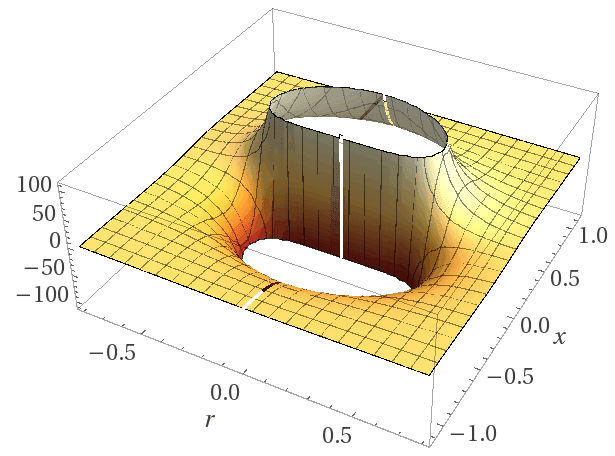
\includegraphics[width=\textwidth]{Pictures/Figure_primitivePlot.png}}
	  					\caption{\small $\hat{\varphi}\in C^\infty (\mathbb{R}^{n+1}\setminus{0})$ \\ in cylindrical coordinates $(x=x^0,r)$}
						\end{figure}		
					}
				%
	 	 	\end{column}
 	 \end{columns}






	


\end{frame}
\note[itemize]{
	\item
}
%-------------------------------------------------------------------------------------------------------------------------------------------------

%-------------------------------------------------------------------------------------------------------------------------------------------------
\begin{frame}[fragile]{HCMM for spheres \underline{(Transitive example)} \hfill\hyperlink{frame:leoresults}{\beamerreturnbutton{}}} \label{frame:TransExample}

	\begin{claimblock}[]
	Explicit HCMM for $SO(n+1) \circlearrowleft \left( S^{n}, \omega\right)$ \qquad($n$ even)
	\end{claimblock}
	\begin{columns}
	%
		\begin{column}{.4\linewidth}
			\begin{itemize}
				\item			Choose basis in $\mathfrak{so}(n)$:	
			\end{itemize}		
		\end{column}
		%
		\begin{column}{.65\linewidth}
	\[
	A_{a b} =(-)^{1+a+b}\left(
	\resizebox{.35\linewidth}{!} 
		{
			\bordermatrix{
								& &\scriptstyle a & & \scriptstyle b & \cr
               	& 0 &    & \cdots &  & 0 \cr
              \scriptstyle a	& 0  &  \cdots & 0 & 1 & 0\ \cr
               	& 0 &   & \cdots &  & 0\cr
              \scriptstyle b	& 0 & -1 & 0 & \cdots & 0 \cr
               	& 0  &   & \cdots &  & 0 }
		}
  \right)
  \]		
		\end{column}
	\end{columns}
	%
	\pause
	\vfill
	\begin{columns}
		\begin{column}{.4\linewidth}
			\begin{itemize}
				\item 			Fundamental vector fields:
			\end{itemize}
		\end{column}
		\begin{column}{.65\linewidth}
			\[v_{A_{a b}}=  (-1)^{1+a+b}\left(x^a \partial_b - x^b \partial_a\right)\]
		\end{column}	
	\end{columns}
	\pause
	\vfill
	\begin{columns}
		\begin{column}{1.05\linewidth}
			\begin{itemize}
				\item From the vanishing of $H^1(G),H^2(G)$ one gets:
				\begin{empheq}[box=\fbox]{align*}
					f_1 (A_{a b}) &= 
					- \iota(v_{F^1(A_{a b})}) \omega =
				\dfrac{1}{n-2}\sum_{k=1}^n \iota(v_{A_{k b}})\iota(v_{A_{k a}})\omega.				
					\\
					f_2(A_{a b} \wedge A_{c d}) &= 
					\dfrac{-1}{4}
						\sum_{k=1}^n	
					\left(
						\iota(v_{A_{k a} \wedge A_{k b} \wedge A_{c d}}) - 
						\iota(v_{A_{a b}\wedge A_{k c} \wedge A_{k d}})
					\right)\omega\\
					f_2(A_{j a} \wedge A_{j b}) &= \dfrac{-1}{n-2}
					\sum_{k=1}^n	
					\left(
						\iota(v_{A_{k a}\wedge A_{j b}\wedge A_{k j}})
					\right)\omega.
				\end{empheq}
				\pause
				\item 	Construction of $f_k$ with $k\geq 3$ can be addressed numerically.
			\end{itemize}
		\end{column}
	\end{columns}



\end{frame}
\note[itemize]{
	\item 	
	First 2 component of HCMM for $SO(n+1)$ on $S^{n}$ (Going higher can be set up as a computational problem - we have a sketch of code in Python -, the first 2 component are easier due to the vanishing of the first two CE cohomology group of $G$)

	\item Recall that $\mathfrak{so}(n)$ is the Lie sub-algebra of $\mathfrak{gl}(n,\mathbb{R})$ consisting of all skew-symmetric square matrices. A basis can be constructed as follows:
\begin{equation}\label{eq:standard-basis}
	\mathcal{B}\coloneqq \big\lbrace 	A_{a b} = (-1)^{1+a+b} \left( E_{a b} - E_{b a}\right)
	\quad \vert \quad 1\leq a<b\leq n \big\rbrace
\end{equation}
where $E_{a b}$ is the matrix with all entries equal to zero and entry $(a,b)$ equal to one.
\item The fundamental vector field of $A_{a b}$ associated to the linear action of $SO(n)$ on $\mathbb{R}^n$ reads as follows:
\begin{displaymath}
	v_{A_{a b}}= \sum_{i,j}[A_{a b}]_{i j}x^j \partial_i  = (-1)^{1+a+b}\left(x^a \partial_b - x^b \partial_a\right)
\end{displaymath}
	\item from the vanishing of the first cohomology group of $(SO(n))$ one can give the action of $f_1$ and of $f_2$ (given on the only two subset of generators such that the image does not vanish)
	\item \textbf{$f_k$ for any $SO(n)$ and $k\geq 3$}:\\
	We know from Theorem \ref{thm:son-cohomology} that $H^3(\mathfrak{so}(n))$ never vanishes... how can we proceed? Tony drafted a code in Python. The repository is still private
}
%-------------------------------------------------------------------------------------------------------------------------------------------------









%===================================================================================
\subsection{Work Done with Marco}
%===================================================================================









%===================================================================================
\subsection{Work Done with Mauro}
%===================================================================================

%------------------------------------------------------------------------------------------------
  \begin{frame}{Hydrodynamical homotopy co-momentum map (details 1) \hfill\hyperlink{frame:hydro2}{\beamerreturnbutton{}}}\label{frame:hydromomap-details}
  	\begin{claimblock}
  		Explicit construction of an HCMM for $SDiff_0 \circlearrowright (\mathbb{R}^3,\nu)$
  	\end{claimblock}
	\begin{columns}
		\begin{column}[c]{.5\linewidth}
		  	\begin{itemize}
		  		\item The observables are  $$L= \Omega^1_{\textrm{ham}}(\mathbb{R}^3)\oplus\Omega^0(\mathbb{R}^3)$$
		  		\item HCMM consists of a pair of functions:
					\begin{align*}
						f_1 &\colon \mathfrak{g} \rightarrow \Omega^1_{\textrm{ham}}(\mathbb{R}^3) \\
						f_2 &\colon \mathfrak{g}\wedge\mathfrak{g} \rightarrow C^\infty(\mathbb{R}^3)
					\end{align*}	
		  	\end{itemize}
		\end{column}	
	  	\hfill  	
		\begin{column}[c]{.5\linewidth}
  		\includestandalone[width=\textwidth]{Pictures/Figure_Euclid_Trigger}
 	 	\end{column}
 	 \end{columns}
 	\begin{columns}
		\begin{column}[c]{.8\linewidth}
		 	 \begin{itemize}
				\item Satisfying the following system:
					\begin{displaymath}
						\begin{cases}
							\textrm{d} f_1(\xi) = \iota_\xi \nu = -\alpha^1(\xi) \\
							\textrm{d} f_2(\xi_1 \wedge \xi_2) = f_1\left([\xi_1,\xi_2]\right) - \iota_{\xi_2}\iota_{\xi_1} \nu 
							 := \mu_2(\xi_1,\xi_2)\\
							f_2\left(\partial \xi_1 \wedge \xi_2 \wedge \xi_3 \right) = \iota_{\xi_3}\iota_{\xi_2}\iota_{\xi_1} \nu
						\end{cases}
					\end{displaymath}
		 	 \end{itemize}
 	 	\end{column}
		\begin{column}[c]{.2\linewidth}
 	 	\end{column}
 	 \end{columns}
  \end{frame}
	\note[itemize]{
		\item (Regarding the diagram)
		\item On the left there is the part of the Chevalley-Eilemberg complex that interact with the L-$\infty$ algebra of observables.
		\item On the right there is the whole de Rham complex of the manifold $M=\mathbb{R}^3$.
		\item Even if only $\Omega^1$ and $\Omega^0$ take part in the definition of a $HCMM$, the Riemmanian structure determine a correspondence with the rest of the de Rham complex.
		\item In order to give an HCMM for this action is necessary to give a solution of the system of 3 equations below.
		\item Recall: $ 	\ast: \Omega^k \rightarrow \Omega^{n-k}$ where $\ast \sigma$ is defined as the unique form such
		 that $ \omega \wedge \ast \sigma = \nu \lbrace \omega, \sigma \rbrace$ where 
		 $\langle,\rangle$ is the inner product on forms induced by the metric. 
	}  
%---------------------------------------------------------------------------------------------------------------------------------------------------


%--------------------------------------------------------------------------------------------------------------------------------------------------- 
  \begin{frame}[t]{Explicit Construction of the hydrodynamical HCMM \hfill\hyperlink{frame:hydro2}{\beamerreturnbutton{}}}
		\begin{enumerate}
			\item<1-> Fix $\vec{b} \in \mathfrak{g}$ and define $f_1(b) := -\vec{A}^\flat$.\\ 
				The first equation is equivalent to solve
				\begin{displaymath}
					\tag{equation of magnetostatic}
					{\rm curl}(\vec{A})=\vec{b}
				\end{displaymath}
				This equation admits a solution 
				\begin{displaymath}
					\tag{Biot-Savart law}
					\vec{A}(r) = \int\frac{\vec{b}\times(\vec{r}-\vec{r}')}{|\vec{r}-\vec{r}'|^3}\textrm{d}r'
				\end{displaymath}							
				\alert {Defined up to a gradient \emph{(gauge freedom)}}. 
			%
			\item<2-> $\mu_2(\xi_1,\xi_2)$ is closed $\forall \xi\in\mathfrak{g}$ $\xRightarrow[\text{lemma}]{\text{Poincar\'e}}$ is exact.\\
				%Hence it is also exact \emph{(Poincar\'e lemma)}.\\
				Take as $f_2(\xi_1,\xi_2)$ a primitive $0$-form, \alert{determined up to a constant $c(\xi_1,\xi_2)$}.
			%
			\item<3-> Third equation is a priori only true up to a constant $c(\xi_1, \xi_2, \xi_3)$.\\
				The constant is zero since $\nu(\xi_1, \xi_2, \xi_3)$ vanishes at infinity and 
				the same is true for $f_2(\partial q)$ upon solving the related Poisson equation
 				\begin{displaymath}
 			 		\Delta f_2(\partial q) = \Delta \nu(\xi_1, \xi_2, \xi_3)			
 				\end{displaymath}
		\end{enumerate}
  \end{frame}
  \note[enumerate]{
  	\item	
  		\begin{itemize}
		  	\item Exploiting the correspondence between tangent fields and 1-form given by the metric is possible to recast the first equation in a simple vector calculus equation containing  the curl.
		  	\item Such equation is the well-known equation of magnetostatic with admits solution by the Biot-Savart law.
		  	\item In the context of hydrodynamic $A$ can be interpreted as a \emph{velocity field} and $b$ as the corresponding vorticity. (See slide for further details)  		
  		\end{itemize}
  	\item In the language of physics, such primitive form is often called "a potential".
  	\item 
  		\begin{itemize}
  			\item (Notation) $q = \xi_1 \wedge \xi_2 \wedge x_3$.
  			\item Last equation tells us that $f_2(\partial q)$ and $ \nu(q)$ differs by a constant. But since both of them vanish at infinity this constant has to be zero.
  			\item The condition of vanishing at infinity has been imposed in order to fulfil the last equation.
  		\end{itemize}
  	\item[$\triangleright$] This construction can be generalized to oriented Riemannian manifolds with further cohomological condition. 
  		See appendix, pag: \ref{frame:RiemannianGeneralization}.
  }
%---------------------------------------------------------------------------------------------------------------------------------------------------


%---------------------------------------------------------------------------------------------------------------------------------------------------
\begin{frame}[fragile]{Hydrodynamics reinterpretation \hfill\hyperlink{frame:hydro2}{\beamerreturnbutton{}}}\label{frame:HydroHCMM-reinterpretation}
	\label{frame:hydro-reinterpretation}
		Consider the loop spaces $L{\mathbb R}^3$,\\
		%
		\begin{propblock}[HCMM for $G\circlearrowright(\mathbb{R}^3,\nu)$ induces \\an ordinary co-mo.map for $G\circlearrowright (LS,\nu^{\ell})$]
			The HCMM $f \colon \mathfrak{g} \to L_{\infty}(\mathbb{R}^3,\nu)$ previously given
			\emph{transgresses}	 to
			\begin{displaymath}%\tag{Arnol'd-Marsden-Weinstein\\ hydrodynamical co-momentum map}
				\begin{tikzcd}[column sep= small,row sep=0ex]
					\lambda \colon& \mathfrak{g}	\arrow[r]& C^\infty(LS) \\
					& {\mathbf b}	\arrow[r, mapsto]& \displaystyle \lambda_b(\textvisiblespace) =-\oint_{\textvisiblespace} A^\flat = - \oint_{\textvisiblespace} f_1({\mathbf b}) 
					%	\quad \forall \gamma \in LS		
				\end{tikzcd}	
			\end{displaymath}
			that is a  moment map for the induced action $G$ on the pre-symplectic loop space $(LM,\nu^{\ell})$. (Smooth space in the sense of Brylinski)
		\end{propblock}
		\begin{itemize}
			\item $\lambda$ corresponds to \emph{Arnol'd-Marsden-Weinstein hydrodynamical co-momentum map}  defined on $\infty$-dim. manifolds.
			\item<2-> $\Lambda = \left\lbrace \lambda_{\mathbf b} \right\rbrace_{{\mathbf b}\in\mathfrak{g}}$ is, up to sign, the {\it Rasetti-Regge current algebra}
			\item<3-> There is a naturally defined {\it Poisson brackets} on $\Lambda$:
				\begin{displaymath}
					\{ f_1({\mathbf b}), f_1({\mathbf c}) \} (\cdot):= \iota_{\mathbf c} \iota_{\mathbf b} \nu (\cdot)=
						\nu({\mathbf b}, {\mathbf c}, \cdot) = f_1([{\mathbf b},{\mathbf c}])
					-df_2 ({\mathbf b} \wedge {\mathbf c})
				\end{displaymath}
				\centering\footnotesize(Note: $\lambda$ is (infinitesimally) $G$-equivariant, i.e. $	\{\lambda_{\mathbf b}, \lambda_{\mathbf c} \} = \lambda_{[{\mathbf b}, {\mathbf c}]}$)
		\end{itemize}

    
\end{frame}
\note[itemize]{
  	\item[ ] \textbf{How all of this is relevant in Hydrodynamics?}
  	\item The loop space is the manifold, in the sense of Brylinsky, consisting of all smooth loops in ${\mathbb R}^3$.
  	\item Transgression can be seen as a pull-back along the evaluation map 
  		$${\rm ev}: L{\mathbb R}^3 \times {\mathbb R} \ni (\gamma, t) \mapsto \gamma(t) \in {\mathbb R}^3$$
  		  	For further details see appendix, pag: \ref{frame:LoopSpacesTransgression}.
  	\item Note that the (RR) current pertaining to ${\mathbf b} \in {\mathfrak g}$  is independent of the choice of $B$.
  			See appendix, pag: \ref{frame:RRcurrents} for other informations on this concept or \cite{Rasetti1975},\cite{Penna1992} for a deeper account.
  	\item In \cite{Callies2016} is proved a general result asserting that, roughly speaking,
			homotopy co-momentum maps transgress to homotopy co-momentum maps on loop (and even mapping) spaces. Further details in appendix, pag: \ref{frame:TransgressionHCMM}.
	\item Actually, the ansatz for $f_1$ term in the previous construction has been precisely motivated by this phenomenon. 
}
%------------------------------------------------------------------------------------------------




%------------------------------------------------------------------------------------------------
\begin{frame}{Non-Equivariance of the Hydrodynamical HCMM \hfill\hyperlink{frame:hydro2}{\beamerreturnbutton{}}} 
	%
 	\begin{columns}
		\begin{column}[c]{.5\linewidth}	
			\begin{defblock}[$G$-equivariant HCMM]
				$f_i\colon \Lambda^i\mathfrak g\to \Omega^{n-i}(M)$ \\ 
				Ad(G)-equivariant $ \forall i\in\{1,...,n\}$.
			\end{defblock}		
		\end{column}
		\begin{column}[c]{.5\linewidth}	
			\begin{defblock}[$\mathfrak{g}$-equivariant HCMM]
				$\mathcal{L}_{v_x}(f_i(q))=f_i([x,q])$ \\
				\phantom{\hspace{2cm}}$\forall q\in \Lambda^{i}\mathfrak g , \: x\in \mathfrak g$\\
				\footnotesize{Where $[x,\cdot]$ is $ad(x)$ acting  on $\Lambda^\bullet \mathfrak g$}
				%$f_i\colon \Lambda^i\mathfrak g\to \Omega^{n-i}(M)$
			\end{defblock}		
		\end{column}
	\end{columns}
	\pause
	\vfill
	\begin{propblock}[$(f)$ is not $\mathfrak{g}$-equivariant]
		\underline{Proof:} 
		\footnotesize
		Consider in particular $\xi = \vec{b} \in \mathfrak{g}$, one should check 
		\begin{displaymath}
			\begin{split}
				0 = f_1\left( [\xi, \vec{b}] \right)
				\stackrel{?}{=}
				%=?=
				{\mathcal L}_{\xi} f_1({\vec{b}})  = -{\mathcal L}_{\xi} \vec{A}^\flat &=
					- d \iota_\xi \vec{A}^\flat = - d \langle \vec{A}, \vec{b} \rangle_g
				\qquad \forall \xi \in \mathfrak{g} \\
						\text{(vanishing at infinity condition)} &\Rightarrow \langle \vec{A}, \vec{b} \rangle_g = 0
			\end{split}
%		\begin{split}
%					f_1\left( [\xi, \vec{b}] \right) &= 0 \\
%					 ( \forall \xi\in \mathfrak{g}) \quad \parallel ? & \qquad\\
%					{\mathcal L}_{\xi} f_1({\vec{b}})  &= -{\mathcal L}_{\xi} \vec{A}^\flat =
%					- d \iota_\xi \vec{A}^\flat = - d \langle \vec{A}, \vec{b} \rangle_g
%		\end{split}		
		\end{displaymath}
		%
	 	\begin{columns}
			\begin{column}[c]{.7\linewidth}
				(By contradiction), consider $\vec{b}\in\mathfrak{g}$ supported on two linked flux tubes
				$(\text{supp}(\vec{b}) = \Gamma_1 \cup \Gamma_2)$, one gets
		\begin{displaymath}
			\int \langle \vec{A}, \vec{b} \rangle_g = 2 \mathbf{n} \Phi_1 \Phi_2 
			\qquad \text{with} \quad 
			\Phi_i = \int_{S_i} \hat{n} \cdot \vec{b}\, d\sigma
		\end{displaymath}
		where $n \in \mathbb{N}$ \emph{(Gauss linking number)}, results
		$$\mathbf{n} \neq 0 \qquad \Rightarrow \quad {\mathcal L}_{\xi} f_1({\vec{b}}) \neq 0  \quad \Rightarrow \quad\text{\faBomb}$$ 
			\end{column}
			\begin{column}[c]{.45\linewidth}	
				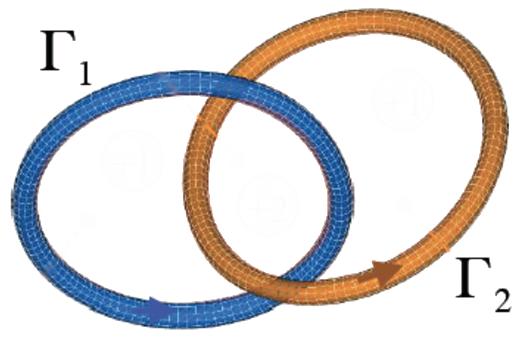
\includegraphics[width=0.9\linewidth]{Pictures/VortexLink}
			\end{column}
		\end{columns}	
	\end{propblock}

		
\end{frame}
\note[itemize]{
    \item We may also naturally ask the question whether the above map $(f)$ is (infinitesimally) {\it G-equivariant}, in the sense of \cite{RWZ}.
    \item In the symplectic case, $G$ connected implies $G$-equivariance. This does not hold true in the multisymplectic case. (ask Leyli!)
    \item In the proof, if $\vec{A}$ is the velocity field of the fluid, $\vec{b}$ is the associated vorticity, the quantity $\langle \vec{A}, \vec{b} \rangle_g$ is called \emph{Helicity}, see below (pag. \ref{Frame:VortexLinks}) for further details.
    \item The proof is by contradiction by exhibiting an example of solenoidal field $\vec{b} = \text{curl}(\vec{A})$ with non vanishing helicity, i.e. not satisfying the condition.\\
    Namely, consider a solenoidal field compactly supported  on a domain $D$ consisting in two disjoint, unknotted but linked closed tubes.
    \item  See \cite{Moffatt-Ricca92} for further elucidation on the non vanishing of the Helicity in the cosidered case.
    Notice that the argument does not depend on the choice of	$\vec{A}$ pertaining to the fixed $\vec{b}$.
    \item The lack of $G$-equivariance is not surprising, since our construction involves Riemannian geometric features.	
}
%------------------------------------------------------------------------------------------------



%------------------------------------------------------------------------------------------------
  \begin{frame}[shrink]{Riemannian Generalization \hfill\hyperlink{frame:hydro2}{\beamerreturnbutton{}}}\label{frame:RiemannianGeneralization}
			\begin{columns}
				\begin{column}{.5\linewidth}
					\begin{itemize}
						\item  $(M,g)$ be a connected compact oriented Riemannian manifold of dimension $n+1$
						\item such that the {\it de Rham} cohomology groups $H_{dR}^{k}(M)$ vanish for $k=1,2,\dots n-1$ 
						\item endow it with the multisymplectic form $\nu$ given by its Riemannian volume form
						\item consider $g_0$, lie algebra consisting of divergence-free vector fields vanishing at a point $x_0 \in M$.
					\end{itemize}
					\begin{claimblock}
						$\exists (f)$, family of HCMM, pertaining to the infinitesimal action of $\mathfrak{g}_0$ on $M$
					\end{claimblock}
				\end{column}
				\begin{column}{.5\linewidth}
 			 		\includestandalone[width=\textwidth]{Pictures/Figure_Riemann_Trigger}
				\end{column}
			\end{columns}
		\textit{Sketch of proof:}\\
			The defining formula triggers a recursive construction starting from $f_1$.\\
			Take $ f_1(\xi) := -\Delta^{-1} \delta (\iota_{\xi} \nu)$
			$\quad$ (...) (see \cite{Miti2018})
  \end{frame}
  		\note[itemize]{
			%\item[(Thm)] A hydrodynamically flavoured HCMM can be similarly construed also for an $(n+1)$-dimensional connected, compact, orientable Riemannian manifold $(M,g)$, upon taking its Riemannian volume form $\nu$ as a multisymplectic form and again the group $G$ of volume preserving diffeomorphism group as symmetry group.
			\item[(recall)] The divergence of a vector field $X$ is defined via ${\rm div}\, X := *d\!*\!X^{\flat} = -\delta X^{\flat} $.
			\item The recursive construction start from $f_1$, up to topological obstructions  since we have a sequence of closed forms, which must be actually exact, together with the constraint $ f_n(\partial q) = (-1)^{\frac{(n+1)(n+2)}{2}}\nu(\xi_1,\dots\xi_{n+1})$, with $q= \xi_1 \wedge \dots \xi_{n+1}$, for the {\it constant} function $\mu_{n+1}(\cdot)$.
				\item A natural candidate for the (n-1)-form $f_1$ can be manufactured via Hodge theory as 
				$f_1(\xi) := -\Delta^{-1} \delta (\iota_{\xi} \nu)$
			after imposing $\delta f_1({\xi}) = 0$ (the analogue of the Coulomb gauge condition).
			\item Condition $H_{dR}^{n-1}(M) = 0$ assure one can safely invert the Hodge Laplacian $\Delta = d\delta + \delta d$;
			\item The 	topological assumptions made ensure that the entire procedure goes through unimpeded due to the formula
			$$
			df_k (\xi_1 \wedge\dots \wedge \xi_k) = \mu_k (\xi_1 \wedge\dots \wedge \xi_k), \qquad \qquad k=2,3,\dots n
			$$
			\item Finally, one has to check that 
			$$
			f_n (\partial (\xi_1 \wedge\dots \wedge \xi_{n+1})) =  -\varsigma(n+1) \iota (\xi_1 \wedge\dots \wedge \xi_{n+1})\nu
			$$
			this is guaranteed by the vanishing of all fields at $x_0$.
			% this is true once we notice that, since $c_{x_0} = 0$, the class $[c_x] = 0$ ( see \cite{Callies2016}, section 9).\qed
		}
%------------------------------------------------------------------------------------------------  



%------------------------------------------------------------------------------------------------
\begin{frame}{A connection with Knot theory \hfill\hyperlink{frame:hydro3}{\beamerreturnbutton{}}}\label{Frame:VortexLinks}
 	\centering$\Rightarrow$\emph{The bridge is the \alert{Vortex Dynamics}}$\Leftarrow$

	\begin{columns}
	\begin{column}[T]{.55\linewidth}
		\vspace{1ex}
 		$\bullet$Consider a perfect (incompressible, inviscid) fluid permeating the  whole space $M=\mathbb{R}^3$.\\
 		\pause
 		$\bullet$ $\text{Physical state} \rightsquigarrow u \in sdiff_0(\mathbb{R}^3)$
% 		\begin{displaymath}
% 			\text{physical state} \rightsquigarrow u \in sdiff_0(\mathbb{R}^3)
% 		\end{displaymath}
 		\begin{columns}
 		\begin{column}{.5\linewidth}	
 			\begin{defblock}[Vorticity]
				$\displaystyle \omega := \textrm{curl}(u)$					
 			\end{defblock}
 		\end{column}
  		\begin{column}{.5\linewidth}	
 			\begin{defblock}[Helicity]
				$\displaystyle h = \int_{\mathbb{R}^3} u \cdot \omega  d^3x$		
 			\end{defblock} 		
 		\end{column}
 		\end{columns}
 				%
  		\begin{columns}
 		\begin{column}{.5\linewidth}	
 			\pause
			$\bullet$ Dynamics is ruled by the \emph{Euler equation}:
			\begin{displaymath}
				\frac{\partial \omega}{\partial t} = [\omega, u]				
			\end{displaymath}
 		\end{column}
  		\begin{column}{.5\linewidth}	
			\begin{propblock}[Helicity is conserved]
				$\frac{d}{dt}H = 0$
			\end{propblock}
 		\end{column}
 		\end{columns}
 			\pause
 			\vspace{2ex}
 			$\bullet$
 			Consider $\omega$ localized in a flux loop $\mathcal{L}$.
 			\begin{propblock}[Vortex filaments are preserved]
 				$\text{supp}(\omega(0))\simeq \text{supp}(\omega(t)) \qquad \forall t$
  			\end{propblock}
	\end{column}
	\begin{column}[T]{.40\linewidth}
		\vspace{-1ex}
		\pause
		\begin{figure}[T]
			\caption{Knotted vortex in water  (Klenecker \& Irvine \cite{Kleckner2013})}
			\href{https://www.nature.com/articles/nphys2560}{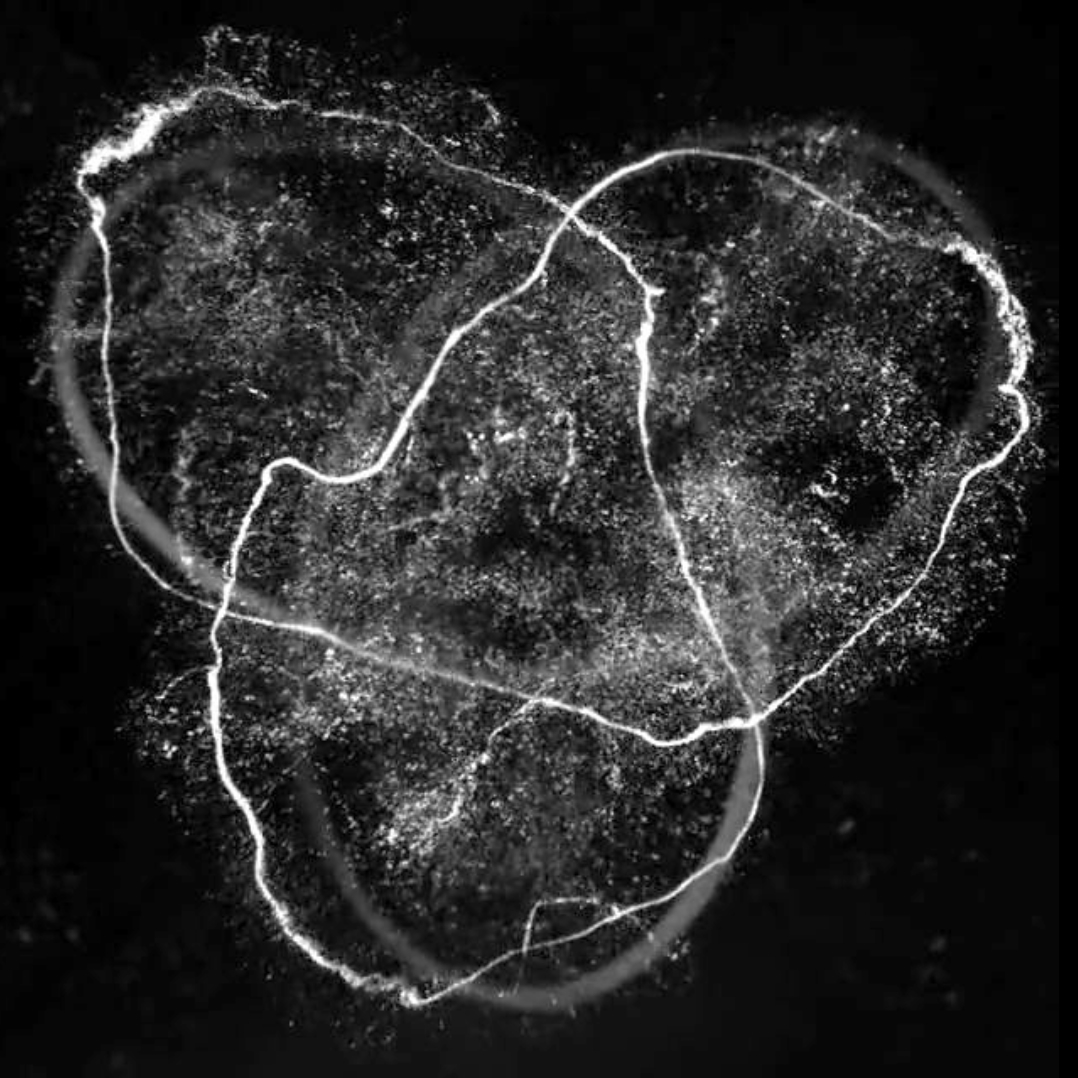
\includegraphics[width=\linewidth]{Pictures/knottedwatervortex}}
		\end{figure}
			\vspace{-2ex}
			\alert{Such fluid configurations are proved to exist both 
			\underline{theoretically} and \underline{experimentally}!}
	\end{column}
	\end{columns} 
\end{frame}
\note[itemize]{
	\item One of the  the main goal of our paper\cite{Miti2018} is to find an application of this construction in knot theory.
	\item The cornerstone of this idea is to recognize the ubiquitous role of the group of preserving diffeomorphisms. 
	The first step is to notice that conserved quantities can be associated to any fluid configurations (especially knotted ones).
 	\item The gist of the second proposition is that the topology of the support of the vorticity is conserved along the fluid evolution.
 	\item The image on the right represents a fluid configuration with knotted vorticity realized in the laboratory.
}
%------------------------------------------------------------------------------------------------


%-------------------------------------------------------------------------------------------------------------------------------------
\subsubsection{Basics of Knot theory}
%-------------------------------------------------------------------------------------------------------------------------------------
  \begin{frame}[fragile]{Basics of \emph{knots theory} \hfill\hyperlink{frame:hydro3}{\beamerreturnbutton{}}}
		\begin{columns}
			\begin{column}[T]{.4\linewidth}
				\begin{figure}
					\caption{Reidmeister's move}
				\ifHandout
				%	\includestandalonewithpath[width=\textwidth,keepaspectratio]{./Pictures}{Figure_trefoil}
				\else
				%	\includestandalonewithpath[width=\textwidth,keepaspectratio]{./Pictures}{Animation_trefoil}
				\fi
				\end{figure}
			\end{column}
				\hfill
			\begin{column}[T]{.6\linewidth}
				\begin{enumerate}
					\item Knots = compact submanifolds of codimension 2 embedded in $\mathbb{R}^3$
						\begin{defblock}[n-link]
							%Disjoint union is written using \coprod, since it is in fact the coproduct in the category of sets.(\amalg)
							$\gamma: {\displaystyle\coprod_1^n S^1 } \to \mathbb{R}^3 $ embedding.				
						\end{defblock}
					\item studied \emph{modulo "ambient isotopies"}
						\begin{defblock}[Ambient isotopies]
							%Disjoint union is written using \coprod, since it is in fact the coproduct in the category of sets.(\amalg)
							$h : {\displaystyle\coprod_1^n S^1 }\times [0,1] \to \mathbb{R}^3 $ smooth homotopy
							s.t. $\hat{h}(t) : {\displaystyle\coprod_1^n S^1 } \to \mathbb{R}^3$ is an embedding $\forall t$	.				
						\end{defblock}	
					\item Holy grail of knot theory: classify all non equivalent (by ambient isotopies) n-links.
					\item \alert{These classes are invariant w.r.t. volume preserving diffeos.}
				\end{enumerate}
				%			
  	  \end{column}
    \end{columns}
	%
 \end{frame}
\note{
	\begin{itemize}
		\item It is possible to build a bridge between knot theory and multisymplectic geometry exploiting the tight connection between both of them with hydrodynamics.\\
		The cornerstone of this relationship is the ubiquitous role of the group of volume preserving diffeomorphisms.
		\item Knot  theory is not simply an instance of studying the topology of loops but the ambient space takes a significant role"
		\item Studying smooth knots is equivalent to study \href{http://mathworld.wolfram.com/PolygonalKnot.html}{tamed polygonal knots}.
		\item choosing a smooth parametrization is tantamount to fix an orientation of the knot.
	\end{itemize}
}
%-------------------------------------------------------------------------------------------------------------------------------------

%-------------------------------------------------------------------------------------------------------------------------------------
\subsubsection{Intermezzo: Poincare duals}
%------------------------------------------------------------------------------------------------

%------------------------------------------------------------------------------------------------
\begin{frame}{Recall: De Rham currents \hfill\hyperlink{frame:hydro3}{\beamerreturnbutton{}}}
	On smooth manifolds is possible to mimick the basic definition of distribution using differential forms:
		\begin{defblock}[De Rham k-Currents]
			\begin{displaymath}
				\mathcal{D}_k(M)
				:= 
			\biggr\{\eta: \Omega^k_c(M)\rightarrow \mathbb{R} \; \left\vert \; \text{\stackanchor{(seq.) continuous}{linear functionals}} \right\} 
				\cong
				\left(\Omega^k_c (M) \right)^\ast
			\end{displaymath}
		\end{defblock}
		%
		\vspace{-2.5ex}
		%
  	\onslide<2->{
  	\begin{columns}
		\begin{column}[t]{.5\linewidth}	
			\begin{defblock}[Annihilation set of $T \in \mathcal{D}$]
				Open subset $A \subset M$ s.t. \\ 
				$\langle T, \phi \rangle = 0 \quad \forall \phi 	
				\text{ s.t. } \text{supp}(\phi) \subset A$
			\end{defblock}
		\end{column}
		\begin{column}[t]{.5\linewidth}			
			\begin{defblock}[Support of $T \in \mathcal{D}$]
				$\text{supp}(T)$ = complement of the union of all open annihilation sets of $\eta$
			\end{defblock}
		\end{column}
  	\end{columns}
  	}		
%
  	\onslide<3->{
	  	We have the analogue of \emph{regular distributions}
			\begin{alignat*}{2}
			  D:\Omega^k(M) & \longrightarrow & \mathcal{D}^{n-k}(M) & \\
			  \eta & \longmapsto & D_\eta & \quad:\quad 
			  \langle D_\eta, \text{\textvisiblespace} \rangle = 
			  \int_M \blank \wedge \eta \\
			  \text{d}\sigma& \longmapsto & D_{\text{d}\sigma} & \quad:\quad 
			  \langle D_{\text{d}\sigma}, \blank \rangle = 
			  (-)^{k} \int_M   \text{d}\blank \wedge\sigma
			\end{alignat*}	  	
  	}				
		%
		\vspace{-2.5ex}
		%
  	\onslide<4->{
		\begin{defblock}[De Rham boundary operator]
			\begin{displaymath}
				\partial : \mathcal{D}_k(M) \rightarrow \mathcal{D}_{k-1}(M) \qquad \text{s.t.} \quad
				\langle \partial T, \blank \rangle = (-)^{k} \langle T, \text{d}\blank \rangle
			\end{displaymath}
		\end{defblock}
  	}							
\end{frame}
\note[itemize]{
	\item this is the analogue of the theory of distribution on $\mathbb{R}^n$
	\item Continuity in the sense of distributions means \emph{sequentially continuous} i.e
		If a sequence $\omega_{k}$ of smooth forms, all supported in the same compact set, is such that all derivatives of all their coefficients tend uniformly to 0 when 
		$k$ tends to infinity, then $T(\omega_{k})$ tends to 0.
	\item $\Omega^k_c(M)$ stands for compact supported k-forms.
	\item Recall the definition of \emph{support} of a differential form
		$$
			\text{supp}(\omega) := \overline{\lbrace p \in M \; \vert \: \omega_p = 0 \rbrace}
		$$
	\item from the definition of regular distribution we obtain the definition of boundary operator.	
	\item De Rham distributions build up a chain complex which is dual (modulo a sign) to the de Rham co-chain complex.
}
%------------------------------------------------------------------------------------------------



%------------------------------------------------------------------------------------------------
\begin{frame}{Recall:Poincaré duals \hfill\hyperlink{frame:hydro3}{\beamerreturnbutton{}}}
	\label{frame:poinduals}
	Given a compact, oriented embedded k-dim submanifold $\Sigma$ of $M$ (n-dim)
	\begin{displaymath}
		\left( i : 	\Sigma \hookrightarrow M \right) \in \text{Emb}_c(k)
	\end{displaymath}		
	you can associate a compactly supported \emph{DeRham current} $D_\Sigma$ defined as
	\begin{displaymath}
		\langle D_\Sigma, \omega\rangle = \int_\Sigma i^\ast (\omega) \qquad 
		\forall \omega \in \Omega^k
	\end{displaymath}
		%
		\vspace{-2.5ex}
		%
	\onslide<2->{
  	\begin{columns}
		\begin{column}[c]{.5\linewidth}	
			\begin{claimblock}
				$\partial D_\Sigma = (-)^{k-1} D_{\partial \Sigma}$ 
			\end{claimblock}
		\end{column}
		\begin{column}[c]{.5\linewidth}			
			\begin{claimblock}
				$ D_{\Sigma_1} \wedge D_{\Sigma_2} = D_{\Sigma_1 \cap \Sigma_2}$
			\end{claimblock}
		\end{column}
  	\end{columns}
  }		
	%
	\onslide<3->{
		\begin{table}[]
		\begin{tabular}{lll}
			Analogue of the Dirac delta function localized on $\Sigma$ & $\Rightarrow$ & 
			\alert{\faWarning \quad not regular \quad \faWarning}
		\end{tabular}
		\end{table}

		We're interested in a \emph{regular approximation} (regularization)
		\begin{defblock}[a (smooth) Poincaré dual of $\Sigma$]
		 $\eta_\Sigma \in \Omega^k$ supported on a tubular neighbourhood $T$ of $\Sigma$ s.t.
		 \begin{displaymath}
				\langle D_{\eta_\Sigma},\omega\rangle \equiv \int_M \omega \wedge \eta_\Sigma =
				\int_T i^\ast \omega \sim 
				\langle D_{\Sigma},\omega\rangle 
		 \end{displaymath}
		\end{defblock}		
		  	\centering \alert{\faWarning  \; ( Not unique! ) \; \faWarning }

  }		
\end{frame}
\note[itemize]{
	\footnotesize
	\item $\forall$ compact submanifold (dim=k) of $M$ (dim= n) one can associates a unique
	 de Rham current. 
	They can be understood as \emph{generalized} differential $(n-k)$-forms concentrated on $\Sigma$.
	This is the analogue of the Dirac delta function localized on $\Sigma$.
	\item Usual definition of Poincar\'e dual (in algebraic topology) is different:
	\\
		%\begin{defblock}[Poincaré dual of $\Sigma$]
			Unique $[\eta_\Sigma ] \in H^{n-k}_c(M)$ s.t.
			\begin{displaymath}
				\int_\Sigma i^\ast \omega = \int_M \omega \wedge \eta_\Sigma \qquad \forall [\omega] \in H^k(M)
			\end{displaymath}
		%\end{defblock}
		More conceptually, Poincaré duals can be seen as \emph{Thom Classes}.
	
	\item Proof of claim 1 is direct:
		\begin{displaymath}
			(-)^{k-1} \langle \partial D_\Sigma , \omega \rangle = 
			\langle D_\Sigma, d\omega\rangle =
			\int_\Sigma i^\ast d \omega = 
			 \int_\Sigma d i^\ast \omega = 
			 \int_{\partial \Sigma} i^\ast \omega =
			\langle D_{\partial \Sigma}, \omega \rangle
		\end{displaymath}
	\item Claim 2 is better understood with smooth Poincarè duals:
		\begin{displaymath}
			\text{supp}(\eta_1 \wedge \eta_2) \subset
			\text{supp}(\eta_1) \cap \text{supp}(\eta_2) \subset
			T_{\Sigma_1 \cap \Sigma_2} \quad\Rightarrow\quad
			\eta_1 \wedge \eta_2 = \eta_{\Sigma_1 \cap \Sigma_2}	
		\end{displaymath}				
		An example: 
		Take as $\Sigma_1$ the $z$-line in $\mathbb{R}^3$, $\eta_1 = \delta_{\{x=y=0\}}	dx \wedge dy$, and as $\Sigma_2$ the $xy$-plane, $\eta_2= \delta_{\{z=0\}} dz$.
		You get $\eta_1 \wedge \eta_2 = \delta_{\{x=y=z=0\}} dx \wedge dy \wedge dz = \eta_{\Sigma_1 \cap \Sigma_2}$
}
%------------------------------------------------------------------------------------------------



%------------------------------------------------------------------------------------------------
\begin{frame}{Relation with Gauss linking number \hfill\hyperlink{frame:hydro3}{\beamerreturnbutton{}}}
		%
		\vspace{-2.5ex}
		%
  	\begin{columns}
		\begin{column}[t]{.5\linewidth}	
			\begin{defblock}[Chern-Simons 3-form]
				$$
					CS({L}) :=  v_{L} \wedge  \omega_{ L} 
				$$
			\end{defblock}
		\end{column}
		\begin{column}[t]{.5\linewidth}	
			\begin{defblock}[Helicity]
				$$
 					{\mathcal H}(L) = \int_{\mathbb{R}^3} CS({L})
				$$
			\end{defblock}						
		\end{column}
  	\end{columns}
	\pause
	\begin{propblock}[
		Choosing a parametrization $\mathbf{r}_i$ (in standard coordinates) for each $L_i$ 
		\begin{displaymath}
			{\mathcal H}(L)  = 
			\sum_{i,j=1}^n
			\,\frac{1}{4\pi}
			\oint_{\gamma_i}\oint_{\gamma_j}
			\frac{\mathbf{r}_i - \mathbf{r}_j}{|\mathbf{r}_i - \mathbf{r}_j|^3}
			\cdot (d\mathbf{r}_i \times d\mathbf{r}_j) =
			\sum_{i,j=1}^n \ell(i,j)
		\end{displaymath}
			$\bullet$ $\ell(i,j) = \ell(j,i)$ : Gauss linking number of components $L_i$ and $L_j$ if $i\neq j$\\
			$\bullet$ $\ell(j,j)$ : {\it framing} of $L_j$\\ 
			\phantom{-------}\footnotesize{ (i.e. $\ell(L_j, L_j^{\prime})$ with $L_j^{\prime}$ being a section of the normal bundle of $L_j$.)}\normalsize

		]
	\pause
  	\begin{columns}
		\begin{column}[c]{.7\linewidth}	
		\underline{Sketch}: Cosider a Hopf Link
			\begin{displaymath}
				L(C,C') = \eta_C \wedge \eta_{\Sigma'} + \eta_{C'} \wedge \eta_\Sigma =
				\eta_{P'} + \eta_{P}
			\end{displaymath}
		\end{column}
		\begin{column}[c]{.25\linewidth}	
			\centering{
			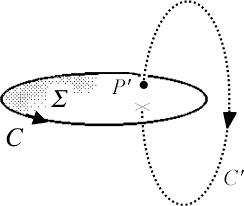
\includegraphics[width=0.75\linewidth]{./Pictures/GaussLink}
			}
		\end{column}
  	\end{columns}
			Therefore $\int L(C,C') = \ell(C,C')$ is counting the times that a knot cross another Seifert surface with sign given by the orientation.
		\end{propblock}
		
\end{frame}
\note[itemize]{
	\item Our previous construction is heavily dependent on a lot of choices 
	but we end up with a quantity that only depends on the starting n-link.
	\item ${\mathcal H}(L)$ is invariant under ambient isotopies.\\
	However, non ambient isotopic links do not necessarily yield different linking numbers
	(it is not an universal invariant!).
  	\begin{columns}
		\begin{column}[c]{.5\linewidth}	
			\centering{
			%
\includegraphics[width=0.5\linewidth]{./Pictures/UnknotsGauss}
			}
		\end{column}
		\begin{column}[c]{.5\linewidth}	
			\centering{
			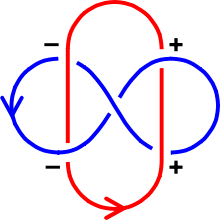
\includegraphics[width=0.35\linewidth]{./Pictures/WhiteheadGauss}
			}
		\end{column}
  	\end{columns}	
	\item
		\begin{displaymath}
	\begin{split}
		\text{link}(\gamma_1,\gamma_2) &=\,\frac{1}{4\pi}
		\oint_{\gamma_1}\oint_{\gamma_2}
		\frac{\mathbf{r}_1 - \mathbf{r}_2}{|\mathbf{r}_1 - \mathbf{r}_2|^3}
		\cdot (d\mathbf{r}_1 \times d\mathbf{r}_2)\\[4pt]
		 &= \frac{1}{4\pi}\int_{S^1 \times S^1} \frac{\text{det}(\dot{\gamma_1}(s),
	 \dot{\gamma_2}(t),\gamma_1(s)-\gamma_2(t))}{|\gamma_1(s)-\gamma_2(t)|^3}\, ds \, dt
	\end{split}
	\end{displaymath}			
}
%------------------------------------------------------------------------------------------------

%------------------------------------------------------------------------------------------------
\begin{frame}{Cohomological interpretation of the linking number \hfill\hyperlink{frame:hydro3}{\beamerreturnbutton{}}}\label{frame:highorderlinking}
		\vspace{2ex}
  	\begin{columns}
		\begin{column}[c]{.75\linewidth}	
			$\bullet$ Choose a pair of linked knots (part of a more complex link).
			Define
			$$ \Xi_{1 2} := - v_{L_1} \wedge v_{L_2} \in \Omega^2(\mathbb{R}^3)$$
			you get:
			\begin{displaymath}
				\begin{split}
				d \Xi_{1 2} =& -\omega_1 \wedge v_2 + v_1 \wedge \omega_2 = CS({L_1\cup L_2}) - 
				\text{"\stackanchor{self}{linking}"}
				\\
				&\Rightarrow \int d \Xi_{1 2} = \ell(1,2)
				\end{split}
			\end{displaymath}		
		\end{column}
		\begin{column}[c]{.20\linewidth}	
			\centering{
			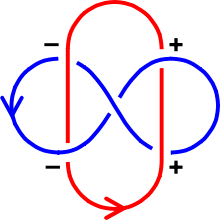
\includegraphics[width=\linewidth]{./Pictures/WhiteheadGauss}
			}
		\end{column}
  	\end{columns}	
	\pause	
	\vspace{1ex}
	$\bullet$ While $\Xi_{1 2}$ is not uniquely defined,it determines an unique class in the \emph{cohomology of the link}
	(independent of the choices)
	\begin{displaymath}
		\langle L_1, L_2 	\rangle := 
		\left[\Xi_{1 2}\big\vert_{S^3\setminus L} \right] \in H^2(S^3\setminus L)
	\end{displaymath}
	\pause
	\vspace{-2ex}
  	\begin{columns}
		\begin{column}[c]{.7\linewidth}	
			\begin{propblock}[$\ell(1,2)= 0 \Leftrightarrow \langle L_1, L_2 \rangle = 0$]
				\vspace{-4ex}
				\begin{displaymath}
				\begin{split}
					l(1,2)=0 ~&\Leftrightarrow~ d \Xi_{1 2} = 0 \in \Omega^2(\mathbb{R}^3)\\
					\text{"Poincar\'e lemma"}	
					~&\Rightarrow~ \exists v_{1 2} \;:\; d v_{1 2} = \Xi_{ 1 2}	\\
					[ \Xi_{1 2} ] = 0 \in H^2(\mathbb{R}^3) ~&\Rightarrow~
					\left[\Xi_{1 2}\big\rvert_{S^3\setminus L} \right] = 0 \in H^2(S^3\setminus L)
				\end{split}
				\end{displaymath}		
			\end{propblock}
		\end{column}
		\begin{column}[c]{.4\linewidth}	
	  	\begin{asideblock}[Cohomology groups of a n-Link]%Shades of...
  			\begin{table}[] % http://tablesgenerator.com/
					\begin{tabular}{l}
						$H^0 (S^3 \setminus L) \cong {\mathbb R}$ \\
						$H^1 (S^3 \setminus L) \cong {\mathbb R}^{n}$ \\
						$H^2 (S^3 \setminus L) \cong {\mathbb R}^{n-1}$ \\
						$H^3 (S^3 \setminus L) \cong 0$
					\end{tabular}
				\end{table}
	  	\end{asideblock}
		\end{column}
  	\end{columns}			



	

\end{frame}
\note[itemize]{
	\item The cohomology of a n-link is the de Rham cohomology of $S^3 \setminus L$, 
	where $S^3$ has to be understood as the compactification of the Euclidean space
	\item Being $\Xi_{1 2}$ closed follows from the fact that 
	$\text{supp}(d \Xi_{1 2}) \subseteq L$ \\
	Similarly, you get that all the velocity 1-forms $v_i$ are closed.
	The cohomology classes of these forms, one for each component of the link, 
	are precisely the generators of $H^1 (S^3 \setminus L)$.
	\item Why such a class is called a number? 
	The name follows from the simplest case of $n=2$.
	\item \underline{Upshot:} we can associate to any pair of knots in a link a  cohomology class.
}
%------------------------------------------------------------------------------------------------

%------------------------------------------------------------------------------------------------
\begin{frame}[shrink]{Higher order linking numbers \hfill\hyperlink{frame:hydro3}{\beamerreturnbutton{}}}
	\begin{itemize}
		\item[•] Take a link with 3 or more components
		\item[•] 	assume all ordinary mutual linking numbers vanish: $\langle L_i, L_j \rangle =0$
		\item[•] Out of the primitives obtained in the previous proposition you can manufacture another closed 2-form
	\end{itemize}
		\vspace{-2ex}
  	\begin{columns}
		\begin{column}[c]{.5\linewidth}	
			\begin{defblock}[Massey product]
				$\Xi_{1 2 3} = - v_1 \wedge v_{2 3} - v_{1 2} \wedge v_3 
				\in \Omega^2(\mathbb{R}^3)$
			\end{defblock}
		\end{column}
		\begin{column}[c]{.5\linewidth}	
			\begin{defblock}[Third order linking number (class)]
				$\langle L_1, L_2, L_3 \rangle := 
				\left[\Xi_{1 2 3}\big\rvert_{S^3\setminus L} \right]
				\in H^2(S^3\setminus L)$
			\end{defblock}
		\end{column}
  	\end{columns}			
  	\pause
	The procedure can be iterated (obstructed by the non vanishing of a higher linking number) yielding a hierarchy of pairs
	\begin{displaymath}
		\Xi_I \in \Omega^2 \qquad v_I \in \Omega^1
	\end{displaymath}
	\center
	\footnotesize{(I = multi index constructed out of the set $\{1,\ldots,n\}$ of the $n$-link components)}\normalsize 

	\footnotesize{
	\pause 	\center 	\textbf{-- Applications --}
  	\begin{columns}
		\begin{column}[c]{.45\linewidth}
			Distinguish different links with same (vanishing) Gauss linking number	
			\center
			\begin{tikzpicture}
			\node[inner sep=0pt] (A) at (0,0)
			    {
\includegraphics[width=.35\textwidth]{./Pictures/UnknotsGauss}};
			\node[inner sep=0pt] (B) at (3,0)
			    {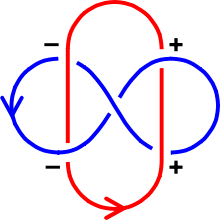
\includegraphics[width=.35\textwidth]{./Pictures/WhiteheadGauss}};
			\draw[draw=none] (A) -- (B)
			    node[midway,fill=white] {$ \not\sim $};
			\end{tikzpicture}
		\end{column}
		\hspace{2ex}
		\begin{column}[c]{.45\linewidth}	
			Ascertain \emph{Brunnian character}
			\centering{
			
\includegraphics[width=0.4\linewidth]{./Pictures/BorromeanLink}
			}
		\end{column}
  	\end{columns}			
	}


\end{frame}
\note[itemize]{
	\item $\Xi_I$ and $v_I$ can be again interpreted via Poincar\'e duality as the smooth Poincar\'e dual of an auxiliary trivial knot and of a corresponding Seifert surface respectively.
	\item Below, two possible application of this machinery are mentioned .
	\item This procedure can be used as a tool to distinguish knots with vanishing linking number. (Figure: two unknots versus a Whithead Link. The latter involve forth order linking numbers computing admitting indices repetition).
	\item Ascertain the Brunnian character of a $n$-link. A link is \emph{Brunnian} 
		or \emph{almost trivial} when it becomes trivial upon removing any component. 
		(Figure: Borromean link).
}
%------------------------------------------------------------------------------------------------

%------------------------------------------------------------------------------------------------
\begin{frame}{Massey products as Conserved quantities \hfill\hyperlink{frame:hydro3}{\beamerreturnbutton{}}}
	%
	\begin{propblock}[
		\quad(1) $\Xi_I$ exact $\Rightarrow$ $v_I$ are hamiltonian (w.r.t volume form) \\
		\phantom{-------------}(2) Massey 2-forms $\Xi_I$ are globally conserved
		]
		\vspace{-4ex}
		\begin{displaymath}
		\begin{split}
			(1)&\quad d v_{I} = \Xi_{I} = \iota_{\xi_{I}} \text{Vol}_{\mathbb{R}^3} \qquad 
			\text{defining}\quad \xi_{I} = \alpha^{-1}(\Xi_{I})
			\qquad \Rightarrow \text{$v_{123}$ Hamiltonian}
			\\
			(2)&\quad \Xi_I \text{ closed} \quad \Rightarrow \quad \mathcal{L}_\xi \Xi_I = d \iota_xi \Xi_I \in B^2
		\end{split}
		\end{displaymath}

	\end{propblock}	
	By construction: the momenta associated to the divergence-free field $\xi_{I}$
	 correspond to $v_I$
		\begin{displaymath}
			v_I = f_1(\xi_I)
		\end{displaymath}
	\pause \vfill
	\begin{propblock}[
		The 1-forms $v_I$ are {\rm first integrals in involution} with respect to the flow generated by the 
		Hamiltonian vector field $\xi_{ L}$, i.e.
		\begin{itemize}
			\item ${\mathcal L}_{\xi_{ L}} v_I = 0$ ($v_I$'s are  {\rm strictly conserved})
			\item $\{v_I, v_J \} = 0$ (for multiindices $I$ and $J$)
		\end{itemize}
	]


	See Thm 6.2 \href{https://arxiv.org/abs/1805.01696}{arXiv: 1805.01696}
	\end{propblock}	
	
	

\end{frame}
\note[itemize]{
	\item $\xi_{123} = \alpha^{-1}(\Xi_{123})$, constructed resorting on the Hodge machinery of $\mathbb{R}^3$ can be regarded as the vorticity field concentrated on a auxiliary knot.
	\item {\bf Proof. Thm 6.2} Using Cartan's formula, we get
		$$
			{\mathcal L}_{\xi_{ L}} v_I = d \iota_{\xi_{ L}} v_I + \iota_{\xi_{ L}} d v_I = 
			d \iota_{\xi_{ L}} v_I  -  \iota_{\xi_{ L}} \iota_{\xi_{ I}} \nu,
		$$
		but the second summand vanishes in view of the general expression
		$$
			\{v_\xi, v_\eta \}(\cdot) = \nu (\xi, \eta, \cdot)
		$$
		and of the peculiar structure of the vector fields involved (they either partially coincide or have disjoint supports). 
		By the same argument, one gets $\iota_{\xi_{ L}} v_I = 0$. From that the the {\it strict} conservation of the $v_I$'s is immediate.\par
	\item  Poincar\'e dual interpretation $\Rightarrow$ $\iota_{\xi_{ L}} v_L = 0$
		$\Rightarrow$ ${\mathcal L}_{\xi_{ L}} v_L = 0 $
		\\
		(this is {\it not} to be expected a priori in multisymplectic geometry)


}
%------------------------------------------------------------------------------------------------





%===================================================================================
\section{TODO: riordinare}
%===================================================================================



%----------------------------------------------------------------------------------------------------------------------------------
\begin{frame}[fragile]{Configuration Space}
  	\begin{columns}[T]
    	\begin{column}{.5\textwidth}		
			\includegraphics<1>[width=\textwidth]{Pics/GeoMec}
			\includegraphics<2->[width=\textwidth]{Pics/GeoMec_noted}
    	\end{column}
    	\begin{column}{.5\textwidth}
			\begin{displaymath}				
   				Q \coloneqq
   				\left\{
				\parbox{45mm}{All possible admissible spatial displacements of a system.}
				 \right\}.
			\end{displaymath}

			\begin{block}<2->{Assumption 1:}
				For point particle $Q$ is a submanifold of $\mathbb{R}^n$.
			\end{block}

			\begin{block}<3->{Assumption 2:}
				Constraints are intrinsically encoded in the geometric structure of $Q$.
			\end{block}

			\vfill
			\begin{alertblock}<4->{Upshot:}
				$Q$ is a \emph{smooth manifold}. 
				Configuration of a system are naturally described by points on it. Configuration coordinates are charts.
			\end{alertblock}
    	\end{column}
  	\end{columns}	
\end{frame}
\note[itemize]{
	\item Consider the set of all possible admissible spatial displacements of a system.
}
%----------------------------------------------------------------------------------------------------------------------------------



%----------------------------------------------------------------------------------------------------------------------------------
\begin{frame}[t]{Symplectic Geometry}
	\begin{exampleblock}{Key point}
		$T^\ast Q$ it's naturally symplectic (i.e. endowed with a closed, bilinear, skew-symmetric form).
		\\
		\underline{Abstraction}: Mechanical systems $\quad \mapsto \quad$ symplectic manifold $(M,\omega)$.
	\end{exampleblock}
	%
	\vfill
  	\begin{columns}[T]
    	\begin{column}{.5\textwidth}	
			\includegraphics<1>[width=1.1\textwidth]{Pics/Fig7} 
			\includegraphics<2->[width=1.1\textwidth]{Pics/Fig8} 		
    	\end{column}
    	\begin{column}{.5\textwidth}
			\begin{itemize}
				\item<1-> Classical observables are elements in $C^\infty(M,\mathbb{R})$
				\item<2-> Observable yields hamiltonian fields $\textrm{d} H = \omega(X_H, \cdot)$
				\item<3-> Trajectories are integral flows of $X_H$
			\end{itemize}
    	\end{column}
  	\end{columns}				
	%
\end{frame}
\note[itemize]{
	\item
    Adunque, tuttalvolta che in concreto voi applicate una sfera materiale a un piano materiale, voi applicate una sfera non perfetta a un piano non perfetto; e questi dite che non si toccano in un punto. Ma io vi dico che anco in astratto una sfera immateriale, che non sia sfera perfetta, può toccare un piano immateriale, che non sia piano perfetto, non in un punto, ma con parte della sua superficie; talché sin qui quello che accade in concreto, accade nell'istesso modo in astratto: e sarebbe ben nuova cosa che i computi e le ragioni fatte in numeri astratti, non rispondessero poi alle monete d'oro e d'argento e alle mercanzie in concreto. Ma sapete, signor Simplicio, quel che accade? Sì come a voler che i calcoli tornino sopra i zuccheri, le sete e le lane, bisogna che il computista faccia le sue tare di casse, invoglie ed altre bagaglie, così, quando il filosofo geometra vuol riconoscere in concreto gli effetti dimostrati in astratto, bisogna che difalchi gli impedimenti della materia; che se ciò saprà fare io vi assicuro che le cose si riscontreranno non meno aggiustatamente che i computi aritmetica Gli errori dunque non consistono né nell'astratto né nel concreto, né nella geometria o nella fisica, ma nel calcolatore, che non sa fare i conti giusti. (G. Galilei, Dialogo sopra i due massimi sistemi, tolemaico e copernicano, a cura di Libero Sosio, Einaudi, Torino, p. 252).

}
%----------------------------------------------------------------------------------------------------------------------------------




%------------------------------------------------------------------------------------------------
\end{document}

	%+----------------------------------------------------------------------------+
%| SLIDES: 
%| Chapter: Bibliography and Figures credit
%| Author: Antonio miti
%| Event: Phd Colloquium - What is ... Geometric mechanics?
%+----------------------------------------------------------------------------+

%- HandOut Flag -----------------------------------------------------------------------------------------
\makeatletter
\@ifundefined{ifHandout}{%
  \expandafter\newif\csname ifHandout\endcsname
}{}
\makeatother

%- D0cum3nt ----------------------------------------------------------------------------------------------
\documentclass[beamer,10pt]{standalone}   
%\documentclass[beamer,10pt,handout]{standalone}  \Handouttrue  

\ifHandout
	\setbeameroption{show notes} %print notes   
\fi

	
%- Packages ----------------------------------------------------------------------------------------------
\usepackage{custom-style}

%--Beamer Style-----------------------------------------------------------------------------------------------
\usetheme{toninus}








%---------------------------------------------------------------------------------------------------------------------------------------------------
%- D0cum3nt ----------------------------------------------------------------------------------------------------------------------------------
\begin{document}
%------------------------------------------------------------------------------------------------


\subsection{References}

%------------------------------------------------------------------------------------------------
% https://en.wikibooks.org/wiki/LaTeX/Bibliographies_with_biblatex_and_biber
\begin{frame}[t,allowframebreaks]{Extended Bibliography}
	%\nocite{*}
	\bibliographystyle{alpha}
	\bibliography{bibfile}
\end{frame}
%------------------------------------------------------------------------------------------------



%------------------------------------------------------------------------------------------------
\begin{frame}[t]{Other aknowledgements}
	\begin{itemize}
		\item Picture - Pendulum 13
			\url{https://andrewjobling.com.au/home-1/everything-okay-becasue-pendulum-swings/}
		\item Picture - Pendulum Phase Space
			\url{https://iopscience.iop.org/article/10.1088/0143-0807/33/2/231}
				\item Picture - Continuum deformation
			\url{https://commons.wikimedia.org/wiki/File:Displacement_of_a_continuum.svg}
		\item Animation - Reidmester moves
			\url{http://realworldmath.tumblr.com/post/57577812688/what-the-hell-is-knot-theory-knot-theory-is-one}
		\item Animation - Bubble rings
			\url{https://www.facebook.com/Nassim.Haramein.official/videos/596203997519126/}
		\item Picture - Whithead link 
			\url{https://en.wikipedia.org/wiki/Whitehead_link}
		\item Picture - Gauss linking number 
			\url{https://www.maths.ed.ac.uk/~v1ranick/papers/ricca.pdf}
		\item Picture - Borromean Rings
			\url{https://en.wikipedia.org/wiki/Borromean_rings}	
	\end{itemize}
\end{frame}
\note[itemize]{
	\item
}
%------------------------------------------------------------------------------------------------



%------------------------------------------------------------------------------------------------
\end{document}
%------------------------------------------------------------------------------------------------










%------------------------------------------------------------------------------------------------
\end{document}

